\chapter{Qubits and quantum gates}
A qubit is a two-dimensional quantum system. The state of a qubit can be represented as a vector in a two-dimensional complex vector space. In this chapter we explore quantum computation in detail. This chapter develops the fundamental principles of quantum computation, and establishes the basic building blocks for quantum circuits a universal language for describing sophisticated quantum computations. This chapter will introduce the fundamental model of quantum computation, the quantum circuit model and the concept that there exists a small set of gates which are universal, that is, any quantum computation whatsoever can be expressed in those gates along with some basic results of quantum computation. 

Many interesting problems are impossible to solve on a classical computer, not because they are in principle insoluble, but because of the astronomical resources required to solve realistic cases of the problem, The spectacular promise of quantum computers is to enable new algorithms which render feasible problems requiring exorbitant resources for their solution on a classical computer. Two broad classes of quantum algorithms are known which fulfill this promise. The first class of algorithms is based upon Shor's quantum Fourier transform, and includes remarkable algorithms for solving the factoring and discrete logarithm problems, providing an exponential speedup over the best known classical algorithms. The second class of algorithms is based upon Grover's algorithm for performing quantum searching. These prodes a less strinig but 


Why are there so few quantum algorithms known which are better than their classical counterparts? The answer is that coming up with good quantum algorithm seems to be a difficult problem. There are at least two reasons for this. First, algorithm design, be it classical or quantum is not easy. The history of algorithms shows us that considerable ingenuity is often required to come up with near optimal algorithms, even for apparently simple problems, like the multiplication of two numbers. Finding good quantum algorithm is made doubly difficult because of the additional constraint that we want our quantum algorithms to be better than the best known classical algorithm. A second reason for the difficult for finding good quantum algorithms is that our intuitions are better adapted to the classical world that they are to the quantum world. If we think about our problems using our native intuition, then the algorithms we come up with are going to be classical algorithms. It takes special insights and special tricks to come up with good quantum algorithms.

To quantify the cost we use the total number of gates required, or the circuit depth. The circuit language also comes with a toolbox of tricks that simpifies algorithm design and provides ready conceptual understanding.

\section{Phase}
`Phase' is a commonly used term in quantum mechanics, with several different meanings dependent upon context. At this point it is convenient to review a couple of these meaning. Consider, for example, the state $e^{\iota \theta}\ket{\psi}$, where $\ket{\psi}$ is a state vector, and $\theta$ is a real number. We say that the state $e^{\iota \theta}$ is equal to $\ket{\psi}$, up to a global phase factor $e^{\iota \theta}$. It is interesting to note that the statistics of measurement predicted for these two states are the same. To see this, suppose $M_m$ is a measurement operator associated to some quantum measurement, and note that the respective probabilities for outcome $m$ occurring are $\bra{\psi}M_m^{\dagger}M_m\ket{\psi}$ and $\bra{\psi}e^{-\iota \theta}M_m^{\dagger} M_m e^{\iota \theta} \ket{\psi}=\bra{\psi}M_m^{\dagger}M_m\ket{\psi}$. Therefore, from an observational point of view these two states are identical. For this reason we may ignore global phase factors are being irrelevant to the observed properties of the physical system.

There is another king of phase known as the relative phase, which has quite a different meaning. Consider the states
\[
\frac{\ket{0}+\ket{1}}{\sqrt{2}}\quad \text{and} \quad \frac{\ket{0}-\ket{1}}{\sqrt{2}}
\]
In the first state the amplitude of $\ket{1}$ is $\frac{1}{\sqrt{2}}$. For the second state the amplitude is $-\frac{1}{\sqrt{2}}$. In each case the magnitude of the amplitude is the same, but they differ in sign. More generally, we say that two amplitudes, $a$ and $b$, differ by a relative phase if there is a real $\theta$ such that $a=exp(\iota \theta)b$. More generally still,two sates are said to differ by a relative phase factor in some basis if each of the amplitudes in that basis is related by such a phase factor. For example, the two states displayed above are the same up to a relative phase shift because the $\ket{0}$ amplitudes are identical (a relative phase factor of $1$), and the $\ket{1}$ amplitudes differ only by a relative phase factor of $-1$. The difference between relative phase factors and global phase factors is that for the relative phase factors the phase factors may vary from amplitude to amplitude. This makes the relative phase a basis-dependent concept unlike global phase. As a result, states which differ only by relative phases in some basis give rise to physically observable differences in measurement statistics, and it is not possible to regard these states as physically equivalent, as we do with states differing by a global phase factor.

\begin{example}
    Express the states $(\ket{0}+\ket{1})/\sqrt{2}$ and $(\ket{0}-\ket{1})/\sqrt{2}$ in a basis in which they are not the same up to a relative phase shift.
    in the $\ket{+}, \ket{-}$ basis they will not be the same even up to a relative phase shift. 
\end{example}





\section{Bloch-Poincare sphere representation of a Qubit}
Consider a Qubit in an arbitrary state $\ket{\psi}=\alpha\ket{0}+\beta\ket{1}$ and $\ket{0}$ and $\ket{1}$ are orthonormal basis states, $\alpha$ and $\beta$ are complex numbers such that $|\alpha|^2+|\beta|^2=1$.
How many real parameters are required to specify the state of a qubit?. Now since $\alpha$ and $\beta$ are complex numbers, we can write them as $\alpha=|\alpha|e^{\iota \phi_{\alpha}}$
and $\beta = |\beta| e^{\iota \phi_{\beta}}$. Here, $|\alpha|$ and $|\beta|$ are real numbers and $\phi_{\alpha}$ and $\phi_{\beta}$ are real numbers. Thus, we need 4 real numbers to specify the state of a qubit.
Now putting the condition that $|\alpha|^2+|\beta|^2=1$, we can write $|\beta|^2=1-|\alpha|^2 \implies |\beta|=\sqrt{1-|\alpha|^2}$.
Thus, we can rewrite the state of a qubit as:
\[ 
    \ket{\psi}=|\alpha|e^{\iota \phi_{\alpha}}\ket{0}+\sqrt{1-|\alpha|^2}e^{\iota \phi_{\beta}}\ket{1}
\]
Now the unknowns are $|\alpha|,\phi_{\alpha},\phi_{\beta}$. Taking $\phi_{\alpha}$ common we get:
\[
    \ket{\psi}=e^{\iota \phi_{\alpha}}\left(|\alpha|\ket{0}+\sqrt{1-|\alpha|^2}e^{\iota(\phi_{\beta}-\phi_{\alpha})}\ket{1}\right)
\]
Now, we know that the state of a qubit is defined upto a global phase. Thus, ignoring the term
$e^{\iota \phi_{\alpha}}$ we can write the state of a qubit as:
\[
    \ket{\psi}=|\alpha|\ket{0}+\sqrt{1-|\alpha|^2}e^{\iota \phi}\ket{1}
\]
where $\phi=\phi_{\beta}-\phi_{\alpha}$ is the relative phase between the states $\ket{0}$ and $\ket{1}$. 
Now, on substituting $|\alpha|=\cos(\theta/2)$, $\sqrt{1-|\alpha|^2}=\sin(\theta/2)$, we get:
\[
    \ket{\psi}=\cos\left(\frac{\theta}{2}\right)\ket{0}+e^{\iota \phi}\sin\left(\frac{\theta}{2}\right)\ket{1}
\]
This cannot be further simplified to reduce the number of variables. Thus, we can clearly see that we need two real numbers - $\theta$ and $\phi$ to specify the state of a qubit.
The state of a qubit can be represented as a point on the surface of a unit sphere in a three-dimensional space. This sphere is called the Bloch Sphere.
A visual representation of the Bloch Sphere (or Bloch-Poincare Sphere) is shown in the figure \ref{fig:bloch_sphere}.

\begin{figure}[ht]
    \centering
    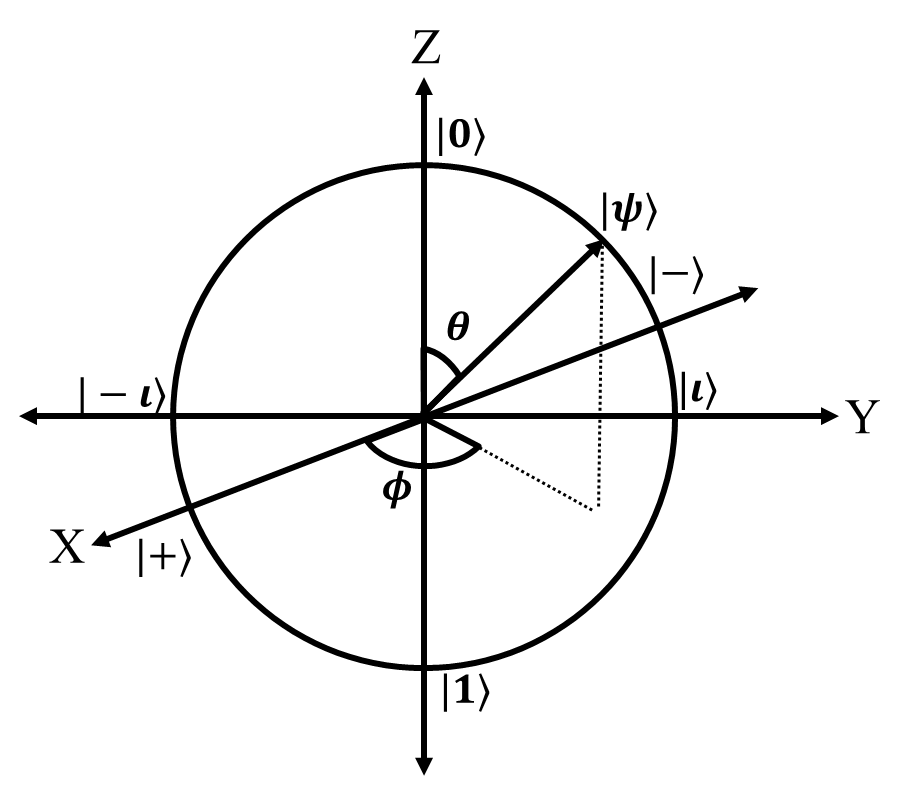
\includegraphics[width=0.6\textwidth]{Images/bloch_sphere_dia.png}
    \caption{Bloch-Poincare Sphere}
    \label{fig:bloch_sphere}
\end{figure}

Thus for different values of $\theta$ and $\phi$ we get different points on the bloch sphere which
represents the different states of a qubit. For a unique mapping from the $\theta$ and $\phi$ to the points on the Bloch Sphere,
we restrict the value of $\theta \in [0,\pi]$ and $\phi \in [0,2\pi]$. 
Thus, the state of a qubit can be represented as:
\[
    \ket{\psi}=\cos\left(\frac{\theta}{2}\right)\ket{0}+e^{\iota \phi}\sin\left(\frac{\theta}{2}\right)\ket{1}
\]
where $\theta \in [0,\pi]$ and $\phi \in [0,2\pi]$ are the polar (represents magnitude or argument) and azimuthal (represents relative phase) angles of the Bloch Sphere respectively.
The following code using Qiskit can be used to plot the Bloch Sphere.
For running the code you need to install the qiskit library. 
%Insert a link 
\href{https://docs.quantum.ibm.com/start/install}{Click here for guide on installing qiskit}
\begin{lstlisting}[language=Python]
import matplotlib.pyplot as plt
from qiskit.visualization import plot_bloch_vector # Import the function to plot the Bloch vector
from qiskit.visualization import plot_bloch_multivector # Import the function to plot the Bloch vector

'''
Function to plot the Bloch Sphere

plot_bloch_vector(bloch, title='', ax=None, figsize=None, coord_type='spherical', font_size=None)

Plots a Bloch Sphere

Parameters
- bloch (list[double]) - array of three elements where [<x>, <y>, <z>] (Cartesian) or 
[<r>, <theta>, <phi>] (spherical in radians) <theta> is inclination angle from +z direction 
<phi> is azimuth from +x direction
- title (str) - a string that represents the title of the plot
- ax (matplotlib.axes.Axes) - an axes of the current figure to plot the Bloch sphere into
- figsize (tuple) - a tuple (width, height) in inches that represents the size of the figure
- coord_type (str) - the coordinate system to use. 'spherical' or 'cartesian', default is cartesian
- font_size (int) - the font size of the tex

Returns
- matplotlib.figure.Figure - a matplotlib figure object

Raises
- ImportError - if matplotlib is not installed
'''

plot_bloch_vector([0,1,0],title='Bloch Sphere')
\end{lstlisting}
The output of the above code is shown in the figure \ref{fig:bloch_sphere_code}.
%Insert a figure
\begin{figure}[ht]
    \centering
    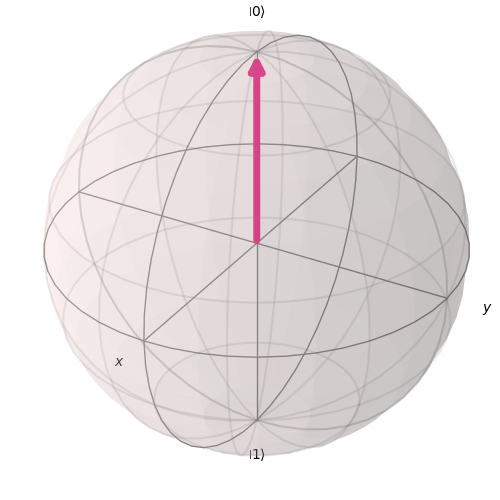
\includegraphics[width=0.5\textwidth]{Images/bloch_sphere.png}
    \caption{Bloch Sphere}
    \label{fig:bloch_sphere_code}
\end{figure}
\textbf{Note that the Bloch Sphere is a geometric representation of the pure states of a qubit. The mixed states of a qubit are represented by the interior of the Bloch Sphere.}

\begin{example}
    The state of a qubit for different values of $\theta$ and $\phi$ is shown in the table \ref{tab:bloch_sphere}.
    \begin{table}[ht]
        \centering
        \begin{tabular}{|c|c|>{\centering\arraybackslash}m{8cm}|c|}
            \hline
            $\theta$ & $\phi$ & State of Qubit & At Axis\\
            \hline
            0 & 0 & $\ket{0}$ & +ve Z\\
            $\pi$ & 0 & $\ket{1}$ & -ve Z \\
            $\frac{\pi}{2}$ & 0 & $\ket{+} = \frac{1}{\sqrt{2}}(\ket{0} + \ket{1})$ & +ve X\\
            $\frac{\pi}{2}$ & $\pi$ & $\ket{-} = \frac{1}{\sqrt{2}}(\ket{0} - \ket{1})$ & -ve X\\
            $\frac{\pi}{2}$ & $\frac{\pi}{2}$ & $\ket{+\iota}=\frac{1}{\sqrt{2}}(\ket{0} + i\ket{1})$ & +ve Y \\
            $\frac{\pi}{2}$ & $-\frac{\pi}{2}$ & $\ket{-\iota}=\frac{1}{\sqrt{2}}(\ket{0} - i\ket{1})$ & -ve Y\\
            \hline
        \end{tabular}
        \caption{State of a Qubit for different values of $\theta$ and $\phi$}
        \label{tab:bloch_sphere}
    \end{table}
\end{example}

\textbf{Quantum Gates acting on Qubits can be thought of as rotations on the Bloch Sphere with some global phase. The global phase is irrelevant to observable quantities and thus does not impact the practical interpretation of the rotation as a transformation on the Bloch sphere. In other words, doing matrix vector multiplication corresponding to rotation action on qubits is the same up to a global phase. A matrix-vector multiplication by a matrix corresponding to some rotation and the vector corresponding to the state of qubit will introduce a global phase shift which can be ignored. Thus, it is easier to imagine this as rotations on bloch sphere where we ignore the global phases implicitly. For example, $R_x(\pi)\ket{0}=-\iota \ket{1}$ using matrix vector multiplication and $R_x(\pi)\ket{0} = \ket{1}$ using the fact that rotations o bloch sphere method but both of them are the same states up to a global phase i.e. $-\iota = e^{\iota 3\pi/2} \times 1$.}
This will be explained further in the later sections.

Note that orthonormal states reside at the ends of the diameter of the Bloch Sphere. 
Let a state $\ket{\psi}$ be represented by a point on the Bloch Sphere. The state $\ket{\psi}$ can be written as:
\[
    \ket{\psi}=\cos\left(\frac{\theta}{2}\right)\ket{0}+e^{\iota \phi}\sin\left(\frac{\theta}{2}\right)\ket{1}
\]
Then the state (say $\ket{\psi'}$) exactly opposite on the Bloch sphere will have the state:
\[
    \ket{\psi'}=\cos\left(\frac{\pi+\theta}{2}\right)\ket{0}+e^{\iota \phi}\sin\left(\frac{\pi+\theta}{2}\right)\ket{1}
\]
Thus, upon simplifying we get:
\[
    \ket{\psi'}=\cos\left(\frac{\pi+\theta}{2}\right)\ket{0}+e^{\iota \phi}\sin\left(\frac{\pi+\theta}{2}\right)\ket{1}
\]
\[
    \ket{\psi'}=-\sin \left(\frac{\theta}{2}\right)\ket{0}+e^{\iota \phi}\cos\left(\frac{\theta}{2}\right)\ket{1}
\]
Now taking the inner product of the states $\ket{\psi}$ and $\ket{\psi'}$ we get:
\[
    \braket{\psi|\psi'}=-\sin\left(\frac{\theta}{2}\right)\cos\left(\frac{\theta}{2}\right)+e^{\iota \phi}e^{-\iota \phi}\sin\left(\frac{\theta}{2}\right)\cos\left(\frac{\theta}{2}\right)=0
\]
Thus, the inner product is zero which implies that the states on the opposite ends of the Bloch Sphere are orthogonal.

\textbf{Note: Such a correspondence does not exist for higher dimensions i.e. No such visualization exists for say Qudits which is d level quantum systems.}
From figure \ref{fig:bloch_sphere} we can see that to convert from polar to cartesian coordinates we use the following relations:
\[
    x=r\sin\theta\cos\phi
\]
\[
    y=r\sin\theta\sin\phi
\]
\[
    z=r\cos\theta
\]
note that here $r=1$ (from pure states i.e. points on the surface of the sphere). To convert from carteisan to polar coordinates we use the following relations:
\[
    r=\sqrt{x^2+y^2+z^2}
\]
\[
    \theta=\cos^{-1}(z)
\]
\[
    \phi=\tan^{-1}\left(\frac{y}{x}\right)
\]
Let us denote the vector as $\vec{n}=(\sin\theta \cos \phi, \sin \theta \sin \phi, \cos \theta, \cos \theta)$.
Points on a Bloch sphere is alwyas a pure state.


\section{Single Qubit Gates}
As said earlier that quantum gates are unitary operators that act on the state of a quantum system. 
Recall from Appendix that the unitary operators are the ones that preserve the inner product of the vectors and the norm of the vectors i.e. they 
only rotate the vectors in the complex vector space (Rotation matrices in $\mathbb{C}^n$). Thus, a state normalized initially remains in the normalized state and does not change its norm 
upon the action of Unitary gates/operators.
The single qubit gates are the quantum gates that act on a single qubit, represented by 2x2 matrices. Since a quantum state is represented by a column vector (in some basis, generally standard basis). 
A gate is a unitary matrix/transformation 
that acts on the qubit(column vector) and changes its state to some other state.
They are rotations on the Bloch Sphere.
\begin{example}
    Consider a $2 \times 2$ matrix $U$ given as:
    \[
        U=\begin{bmatrix}
            a & b \\
            c & d
        \end{bmatrix}
    \]
    in the orthonormal input and output basis $\{\ket{0},\ket{1}\}$, thus, we can write the matrix $U$ as:
    \[
        U=a\ket{0}\bra{0}+b\ket{0}\bra{1}+c\ket{1}\bra{0}+d\ket{1}\bra{1}
    \]
    This, will be used to express the Pauli Matrices in the later sections.
\end{example}

\subsection{Pauli Matrices}
\subsubsection{Pauli-I Gate}
It is used for the measurement of decoherence (Qubits start to lose its Quantum abilities after certain time).
The Truth table is given as in table \ref{tab:pauli-i}. It does no rotation of the bloch vector on the Bloch Sphere.
%Insert a table
\begin{table}[ht]
    \centering
    \begin{tabular}{|c|c|}
        \hline
        Input & Output\\
        \hline  
        $\ket{0}$ & $\ket{0}$\\
        $\ket{1}$ & $\ket{1}$\\
        \hline
    \end{tabular}
    \caption{Truth Table for Pauli-I Gate}
    \label{tab:pauli-i}
\end{table}
The code for the Pauli-I Gate is as follows:
\begin{lstlisting}[language=Python]
from qiskit import QuantumRegister, ClassicalRegister, QuantumCircuit
from numpy import pi

qreg_q = QuantumRegister(1, 'q')

circuit = QuantumCircuit(qreg_q)

circuit.id(qreg_q[0]) #For Pauli-Identity Gate
circuit.draw(output='mpl')#.savefig('../images/pauli-i.png') #Draw the circuit
\end{lstlisting}
The circuit symbol is as shown in figure \ref{fig:pauli-i}
\begin{figure}[ht]
    \centering
    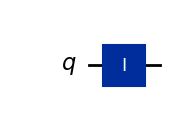
\includegraphics[width=0.3\textwidth]{Images/pauli-i.png}
    \caption{Pauli-I Gate}
    \label{fig:pauli-i}
\end{figure}
In operator Notation it is:
\begin{align*}
    I\ket{0}&=\ket{0} \\
    I\ket{1}&=\ket{1}
\end{align*}
It is represented by the matrix in the computational basis ($\ket{0},\ket{1}$) as:
\[
    \sigma_I=I=\begin{bmatrix}
        1 & 0 \\
        0 & 1
    \end{bmatrix}
\]
It's Eigen values are 1 and 1. It's Eigen vectors are any vector in the 2-D Space.
Note that it's Unitary($II^{\dagger}=I^{\dagger}I=I;I=I^{-1}$) and Hermitian Matrix($I=I^{\dagger}$), thus a Normal Matrix ($II^{\dagger}=I^{\dagger}I$) hence Unitarily digonalizable.
Thus, it has a Spectral decomposition (outer product representation) which can be written as:
\[
    I=\ket{0}\bra{0}+\ket{1}\bra{1}
\]
Action of Pauli-I Gate on a general qubit $\alpha\ket{0}+\beta\ket{1}$ is:
\[
    \begin{bmatrix}
        1 & 0 \\
        0 & 1
    \end{bmatrix}\begin{bmatrix}
        \alpha \\
        \beta
    \end{bmatrix}=\begin{bmatrix}
        \alpha \\
        \beta
    \end{bmatrix}= \alpha\ket{0}+\beta\ket{1}
\]

\subsubsection{Pauli-X Gate}
It is also known as the NOT gate. It is equivalent of Classical NOT Gate.
It is thus called Bit Flip Gate. The truth table is as in \ref{tab:pauli-x}. It does anticlockwise $\pi$ rotation about X 
axis of Bloch sphere. It flips the state $\ket{0}$ to $\ket{1}$ and $\ket{1}$ to $\ket{0}$.
\begin{table}[ht]
    \centering
    \begin{tabular}{|c|c|}
        \hline
        Input & Output\\
        \hline
        $\ket{0}$ & $\ket{1}$\\
        $\ket{1}$ & $\ket{0}$\\
        \hline
    \end{tabular}
    \caption{Truth Table for Pauli-X Gate}
    \label{tab:pauli-x}
\end{table}

The code for the Pauli-X Gate is as follows:
\begin{lstlisting}[language=Python]
from qiskit import QuantumRegister, ClassicalRegister, QuantumCircuit
from numpy import pi

qreg_q = QuantumRegister(1, 'q')
circuit = QuantumCircuit(qreg_q,name='Not Gate')

circuit.x(qreg_q[0])

circuit.draw(output='mpl')#.savefig('../images/pauli-x.png') #Draw the circuit
\end{lstlisting}
The circuit symbol is as shown in figure \ref{fig:pauli-x}.
\begin{figure}[ht]
    \centering
    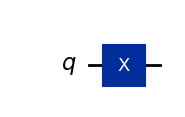
\includegraphics[width=0.3\textwidth]{Images/pauli-x.png}
    \caption{Pauli-X Gate}
    \label{fig:pauli-x}
\end{figure}
In the operator Notation it is:
\begin{align*}
    X\ket{0}&=\ket{1} \\
    X\ket{1}&=\ket{0}
\end{align*}
It is represented by the matrix in the computational basis ($\ket{0},\ket{1}$) as:
\[
    \sigma_X=X=\begin{bmatrix}
        0 & 1 \\
        1 & 0
    \end{bmatrix}
\]
It's Eigen values are 1 and -1. It's corresponding Eigen vectors are $\ket{+}=\frac{1}{\sqrt{2}}(\ket{0}+\ket{1})$ and $\ket{-}=\frac{1}{\sqrt{2}}(\ket{0}-\ket{1})$.
It is a Unitary and Hermitian Matrix. It is a Normal Matrix hence Unitarily Diagonalizable.
It has a Spectral decomposition (outer product representation) which can be written as:
\[
    X=\ket{+}\bra{+}-\ket{-}\bra{-}
\]
Upon, substituting the values of $\ket{+}$ and $\ket{-}$ we get:
\begin{align*}
    X&=\dfrac{1}{\sqrt{2}}(\ket{0}+\ket{1})\dfrac{1}{\sqrt{2}}(\bra{0}+\bra{1})-\dfrac{1}{\sqrt{2}}(\ket{0}-\ket{1})\dfrac{1}{\sqrt{2}}(\bra{0}-\bra{1})\\
    &=\dfrac{1}{2}(\ket{0}\bra{0}+\ket{0}\bra{1}+\ket{1}\bra{0}+\ket{1}\bra{1})-\dfrac{1}{2}(\ket{0}\bra{0}-\ket{0}\bra{1}-\ket{1}\bra{0}+\ket{1}\bra{1})\\
    &=\ket{0}\bra{1}+\ket{1}\bra{0}
\end{align*}
Thus, the Pauli-X Gate can also be written as:
\[
    X=\ket{0}\bra{1}+\ket{1}\bra{0}
\]
\textbf{Note that the Pauli-X Gate can be written as $X=HZH$ or $\sigma_X=H\sigma_Z H$  where $H$ and $Z$ are the Hadamard and Pauli-Z Gates respectively.}
Action of Pauli-X Gate on a general qubit $\ket{\psi}=\alpha\ket{0}+\beta\ket{1}$ is: 
\[
    \begin{bmatrix}
        0 & 1 \\
        1 & 0
    \end{bmatrix}\begin{bmatrix}
        \alpha \\
        \beta
    \end{bmatrix}=\begin{bmatrix}
        \beta \\
        \alpha
    \end{bmatrix}= \beta\ket{0}+\alpha\ket{1}
\]

\subsubsection{Pauli-Y Gate}
It is a anitclockwise $\pi$ rotation about Y axis of Bloch Sphere. 
It flips the Qubit and muultiplies a complex amplitude. The truth table is as in table \ref{tab:pauli-y}.
\begin{table}[ht]
    \centering
    \begin{tabular}{|c|c|}
        \hline
        Input & Output\\
        \hline
        $\ket{0}$ & $i\ket{1}$\\
        $\ket{1}$ & $-i\ket{0}$\\
        \hline
    \end{tabular}
    \caption{Truth Table for Pauli-Y Gate}
    \label{tab:pauli-y}
\end{table}
The code for the Pauli-Y Gate is as follows:
\begin{lstlisting}[language=Python]
from qiskit import QuantumRegister, ClassicalRegister, QuantumCircuit
from numpy import pi

qreg_q = QuantumRegister(1, 'q')
circuit = QuantumCircuit(qreg_q,name='Not Gate')

circuit.y(qreg_q[0]) #Apply the Y gate

circuit.draw(output='mpl')#.savefig('../images/pauli-x.png') #Draw the circuit
\end{lstlisting}

The circuit symbol is as shown in figure \ref{fig:pauli-y}.
\begin{figure}[ht]
    \centering
    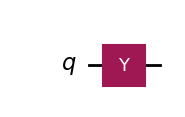
\includegraphics[width=0.3\textwidth]{Images/pauli-y.png}
    \caption{Pauli-Y Gate}
    \label{fig:pauli-y}
\end{figure}
In the operator Notation it is:
\begin{align*}
    Y\ket{0}&=i\ket{1} \\
    Y\ket{1}&=-i\ket{0}
\end{align*}
It is represented by the matrix in the computational basis ($\ket{0},\ket{1}$) as:
\[
    \sigma_Y=Y=\begin{bmatrix}
        0 & -i \\
        i & 0
    \end{bmatrix}
\]
It's Eigen values are 1 and -1. It's corresponding Eigen vectors are $\ket{+i}=\frac{1}{\sqrt{2}}(\ket{0}+i\ket{1})$ and $\ket{-i}=\frac{1}{\sqrt{2}}(\ket{0}-i\ket{1})$.
It is a Unitary and Hermitian Matrix. It is a Normal Matrix hence Unitarily Diagonalizable.
It has a Spectral decomposition (outer product representation) which can be written as:
\[
    Y=\ket{+i}\bra{+i}-\ket{-i}\bra{-i}
\]
Upon, substituting the values of $\ket{+i}$ and $\ket{-i}$ we get:
\begin{align*}
    Y&=\dfrac{1}{\sqrt{2}}(\ket{0}+i\ket{1})\dfrac{1}{\sqrt{2}}(\bra{0}-i\bra{1})-\dfrac{1}{\sqrt{2}}(\ket{0}-i\ket{1})\dfrac{1}{\sqrt{2}}(\bra{0}+i\bra{1})\\
    &=\dfrac{1}{2}(\ket{0}\bra{0}-i\ket{0}\bra{1}+i\ket{1}\bra{0}+\ket{1}\bra{1})-\dfrac{1}{2}(\ket{0}\bra{0}+i\ket{0}\bra{1}-i\ket{1}\bra{0}+\ket{1}\bra{1})\\
    &=i\ket{1}\bra{0}-i\ket{0}\bra{1}
\end{align*}
Thus, the Pauli-Y Gate can also be written as:
\[
    Y=-i\ket{0}\bra{1}+i\ket{1}\bra{0}
\]
\textbf{Note that the Pauli-Y Gate can be written as $Y=\iota XZ$ or $\sigma_Y=\iota \sigma_X\sigma_Z$  where $X$ and $Z$ are the Pauli-X and Pauli-Z Gates respectively.}
This means that the Pauli-Y Gate is a rotation about the Y-axis of the Bloch Sphere by $\pi$ in anticlocwise direction and is equivalent to a rotation about the X-axis by anticlockwise $\pi$ followed by a rotation about the Z-axis by anticlockwise $\pi$
(upto a global phase).

Action of Pauli-Y Gate on a general qubit $\ket{\psi}=\alpha\ket{0}+\beta\ket{1}$ is:
\[
    \begin{bmatrix}
        0 & -i \\
        i & 0
    \end{bmatrix}\begin{bmatrix}
        \alpha \\
        \beta
    \end{bmatrix}=\begin{bmatrix}
        -i\beta \\
        i\alpha
    \end{bmatrix}=i\alpha\ket{1}-i\beta\ket{0}
\]

\subsubsection{Pauli-Z Gate}
It is a anticlockwise $\pi$ rotation about Z axis of Bloch Sphere.
It flips the sign of the $\ket{1}$ state. It is also called Phase Flip/Phase shoft/Sign flip gate.
The truth table is as in table \ref{tab:pauli-z}.
\begin{table}[ht]
    \centering
    \begin{tabular}{|c|c|}
        \hline
        Input & Output\\
        \hline
        $\ket{0}$ & $\ket{0}$\\
        $\ket{1}$ & $-\ket{1}$\\
        \hline
    \end{tabular}
    \caption{Truth Table for Pauli-Z Gate}
    \label{tab:pauli-z}
\end{table}
The code for the Pauli-Z Gate is as follows:
\begin{lstlisting}[language=Python]
from qiskit import QuantumRegister, ClassicalRegister, QuantumCircuit
from numpy import pi

qreg_q = QuantumRegister(1, 'q')
circuit = QuantumCircuit(qreg_q,name='Not Gate')

circuit.z(qreg_q[0]) #Apply the Z gate

circuit.draw(output='mpl')#.savefig('../images/pauli-z.png') #Draw the circuit
\end{lstlisting}
The circuit symbol is as shown in figure \ref{fig:pauli-z}.
\begin{figure}[ht]
    \centering
    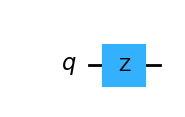
\includegraphics[width=0.3\textwidth]{Images/pauli-z.png}
    \caption{Pauli-Z Gate}
    \label{fig:pauli-z}
\end{figure}
In the operator Notation it is:
\begin{align*}
    Z\ket{0}&=\ket{0} \\
    Z\ket{1}&=-\ket{1}
\end{align*}
It is represented by the matrix in the computational basis ($\ket{0},\ket{1}$) as:
\[
    \sigma_Z=Z=\begin{bmatrix}
        1 & 0 \\
        0 & -1
    \end{bmatrix}
\]
It's Eigen values are 1 and -1. It's corresponding Eigen vectors are $\ket{0}$ and $\ket{1}$.
It is a Unitary and Hermitian Matrix. It is a Normal Matrix hence Unitarily Diagonalizable.
It has a Spectral decomposition (outer product representation) which can be written as:
\[
    Z=\ket{0}\bra{0}-\ket{1}\bra{1}
\]
In Compact form, we can write Pauli-Z Gate as:
\[
    Z\ket{j}=(-1)^j\ket{j}
\]
where $j=0,1$.
Action of Pauli-Z Gate on a general qubit $\ket{\psi}=\alpha\ket{0}+\beta\ket{1}$ is:
\[
    \begin{bmatrix}
        1 & 0 \\
        0 & -1
    \end{bmatrix}\begin{bmatrix}
        \alpha \\
        \beta
    \end{bmatrix}=\begin{bmatrix}
        \alpha \\
        -\beta
    \end{bmatrix}=\alpha\ket{0}-\beta\ket{1}
\]
\begin{example}
    \textbf{(Pauli Matrices: Hermitian and Unitary)} Show that the pauli matrices are Hermitian and unitary.

    We check $I,X,Y,Z$ in turns.
    \[
    I^{\dagger}=\left(\begin{bmatrix} 1 & 0 \\ 0 & 1 \end{bmatrix}^T \right)^* = \begin{bmatrix} 1 & 0 \\ 0 & 1 \end{bmatrix}^* = \begin{bmatrix} 1 & 0 \\ 0 & 1 \end{bmatrix} =I
    \]
    \[
    I^{\dagger}I=II=I
    \]
    \[
    X^{\dagger}=\left(\begin{bmatrix} 0 & 1 \\ 1 & 0 \end{bmatrix}^T \right)^* = \begin{bmatrix} 0 & 1 \\ 1 & 0 \end{bmatrix}^* = \begin{bmatrix} 0 & 1 \\ 1 & 0 \end{bmatrix} =X
    \]
    \[
    X^{\dagger}X=XX=\begin{bmatrix} 0 & 1 \\ 1 & 0 \end{bmatrix} = \begin{bmatrix} 0 & 1 \\ 0 & 1 \end{bmatrix} = I
    \]
    \[
    Y^{\dagger}=\left(\begin{bmatrix} 0 & -\iota \\ \iota & 0 \end{bmatrix}^T \right)^* = \begin{bmatrix} 0 & \iota \\ -\iota & 0 \end{bmatrix}^* = \begin{bmatrix} 0 & -\iota \\ \iota & 0 \end{bmatrix} =Y
    \]
    \[
    Y^{\dagger}Y=YY=\begin{bmatrix} 0 & -\iota \\ \iota & 0 \end{bmatrix} \begin{bmatrix} 0 & -\iota \\ \iota & 0 \end{bmatrix}=\begin{bmatrix} 1 & 0 \\ 0 & 1 \end{bmatrix}
     \]
    \[
    Z^{\dagger}=\left(\begin{bmatrix} 1 & 0 \\ 0 & -1 \end{bmatrix}^T \right)^* = \begin{bmatrix} 1 & 0 \\ 0 & -1 \end{bmatrix}^* = \begin{bmatrix} 1 & 0 \\ 0 & -1 \end{bmatrix} =Z
    \]
    \[
    Z^{\dagger}Z=\begin{bmatrix} 1 & 0 \\ 0 & -1 \end{bmatrix} \begin{bmatrix} 1 & 0 \\ 0 & -1 \end{bmatrix} = \begin{bmatrix} 1 & 0 \\ 0 & 1 \end{bmatrix} = I
    \]
\end{example}

\begin{example}
    Calculate the matrix representation of the tensor products of the Pauli operators (a)$X$ and $Z$; (b)$I$ and $X$; (c) $X$ and $I$. Is the tensor product commutative?

    Using Kronecker product we have,
    \begin{enumerate}
        \item 
        \[
        X\otimes Z=\begin{bmatrix}
            0Z & 1Z \\ 1Z & 0Z
        \end{bmatrix}= \begin{bmatrix}
            0\begin{bmatrix} 1 & 0 \\ 0 & -1 \end{bmatrix} & 1 \begin{bmatrix} 1 & 0 \\ 0 & -1 \end{bmatrix} \\ 1 \begin{bmatrix} 1 & 0 \\ 0 & -1 \end{bmatrix} & 0 \begin{bmatrix} 1 & 0 \\ 0 & -1 \end{bmatrix}
        \end{bmatrix}=\begin{bmatrix} 0 & 0 & 1 & 0 \\ 0 & 0 & 0 -1 \\ 1 & 0 & 0 & 0 \\ 0 & -1 & 0 & 0 \end{bmatrix}
        \]
        \item
        \[
        I\otimes X=\begin{bmatrix}
            1X & 0X \\ 0X & 1X
        \end{bmatrix}= \begin{bmatrix}
            1\begin{bmatrix} 0 & 1 \\ 1 & 0 \end{bmatrix} & 0 \begin{bmatrix} 0 & 1 \\ 1 & 0 \end{bmatrix} \\ 0 \begin{bmatrix} 0 & 1 \\ 1 & 0 \end{bmatrix} & 1 \begin{bmatrix} 0 & 1 \\ 1 & 0 \end{bmatrix}
        \end{bmatrix}=\begin{bmatrix} 0 & 1 & 0 & 0 \\ 1 & 0 & 0 & 0 \\ 0 & 0 & 0 & 1 \\ 0 & 0 & 1 & 0 \end{bmatrix}
        \]
        \item 
        \[
        X\otimes I=\begin{bmatrix}
            0I & 1I \\ 1I & 0I
        \end{bmatrix}= \begin{bmatrix}
            0\begin{bmatrix} 1 & 0 \\ 0 & 1 \end{bmatrix} & 1\begin{bmatrix} 1 & 0 \\ 0 & 1 \end{bmatrix} \\ 1\begin{bmatrix} 1 & 0 \\ 0 & 1 \end{bmatrix} & 0\begin{bmatrix} 1 & 0 \\ 0 & 1 \end{bmatrix}
        \end{bmatrix}=\begin{bmatrix} 0 & 0 & 1 & 0 \\ 0 & 0 & 0 & 1 \\ 1 & 0 & 0 & 0 \\ 0 & 1 & 0 & 0 \end{bmatrix}
        \]
    \end{enumerate}
    Comparing (b) and (c), we conclude and adjoint operations distribute over the tensor product.
\end{example}

\begin{example}
    \textbf{(Commutation relations for the Pauli Matrices)} Verify the commutation relations
    \[
    [X,Y]=2\iota Z;[Y,Z]=2\iota X;[Z,X]=2\iota Y
    \]
    There is an elegant way of writing this using $\epsilon_{jkl}$, the antisymmetric tensor on three indices, for which $\epsilon_{jkl}=0$ except for $\epsilon_{123}=\epsilon_{231}=\epsilon_{312}=1$, and $\epsilon_{321}=\epsilon_{213}=\epsilon_{132}=-1$:
    \[
    [\sigma_j,\sigma_k]=2\iota\sum_{l=1}^3 \epsilon_{jkl}\sigma_l
    \]

    We verify the proposed relations via computation in the computational basis:
    \[
    [X,Y]=XY-YX=\begin{bmatrix} 0 & 1 \\ 1 & 0 \end{bmatrix}\begin{bmatrix} 0 & -\iota \\ \iota & 0 \end{bmatrix} - \begin{bmatrix}0 & -\iota \\ \iota & 0 \end{bmatrix} \begin{bmatrix} 0 & 1 \\ 1 & 0 \end{bmatrix} = \begin{bmatrix} \iota & 0 \\ 0 & -\iota \end{bmatrix} - \begin{bmatrix} -\iota & 0 \\ 0 & \iota \end{bmatrix} =2\iota Z
    \]
    \[
    [Y,Z]=YZ-ZY=\begin{bmatrix} 0 & -\iota  \\ \iota & 0 \end{bmatrix}\begin{bmatrix} 1 & 0 \\ 0 & -1 \end{bmatrix} - \begin{bmatrix} 1 & 0 \\ 0 & -1 \end{bmatrix} \begin{bmatrix} 0 & -\iota  \\ \iota & 0 \end{bmatrix} = \begin{bmatrix} 0 & \iota \\ \iota & 0 \end{bmatrix} - \begin{bmatrix} 0 & -\iota \\ -\iota & 0 \end{bmatrix} =2\iota X
    \]
    \[
    [Z,X]=ZX-XZ=\begin{bmatrix} 1 & 0 \\ 0 & -1 \end{bmatrix}\begin{bmatrix} 0 & 1 \\ 1 & 0 \end{bmatrix} - \begin{bmatrix}0 & 1 \\ 1 & 0 \end{bmatrix} \begin{bmatrix} 1 & 0 \\ 0 & -1 \end{bmatrix} = \begin{bmatrix} 0 & 1 \\ -1 & 0 \end{bmatrix} - \begin{bmatrix} 0 & -1 \\ 1 & 0 \end{bmatrix} =2\iota Y
    \]
\end{example}
\begin{example}
    \textbf{(Anti-commutation relations for the Pauli matrices)} Verify the anti-communal relations
    \[
    \{\sigma_i,\sigma_j\}=0
    \]
    where $i\neq j$ are both chosen from the set $1,2,3$. Also verify that $(i=0,1,2,3)$
    \[
    \sigma_i^2=I
    \]
    We again verify the proposed relations via computation in the computational basis:
    \[
    \{X,Y\}=XY+YX=\begin{bmatrix} 0 & 1 \\ 1 & 0 \end{bmatrix}\begin{bmatrix} 0 & -\iota  \\ \iota & 0 \end{bmatrix}+\begin{bmatrix} 0 & -\iota  \\ \iota & 0 \end{bmatrix}\begin{bmatrix} 0 & 1 \\ 1 & 0 \end{bmatrix}=\begin{bmatrix} \iota & 0 \\ 0 & -\iota \end{bmatrix}+\begin{bmatrix} -\iota & 0 \\ 0 & \iota \end{bmatrix} = \begin{bmatrix} 0 & 0 \\ 0 & 0 \end{bmatrix}
    \]
    \[
    \{Y,Z\}=YZ+ZY=\begin{bmatrix} 0 & -\iota  \\ \iota & 0 \end{bmatrix}\begin{bmatrix} 1 & 0 \\ 0 & -1 \end{bmatrix}+\begin{bmatrix} 1 & 0 \\ 0 & -1 \end{bmatrix}\begin{bmatrix} 0 & -\iota  \\ \iota & 0 \end{bmatrix}=\begin{bmatrix} 0 & \iota \\ \iota & 0 \end{bmatrix}+\begin{bmatrix} 0 & -\iota \\ -\iota & 0 \end{bmatrix} = \begin{bmatrix} 0 & 0 \\ 0 & 0 \end{bmatrix}
    \]
    \[
    \{Z,X\}=ZX+XZ=\begin{bmatrix} 1 & 0 \\ 0 & -1 \end{bmatrix}\begin{bmatrix} 0 & 1 \\ 1 & 0 \end{bmatrix}+\begin{bmatrix} 0 & 1 \\ 1 & 0 \end{bmatrix}\begin{bmatrix} 1 & 0 \\ 0 & -1 \end{bmatrix}=\begin{bmatrix} 0 & 1 \\ -1 & 0 \end{bmatrix}+\begin{bmatrix} 0 & -1 \\ 1 & 0 \end{bmatrix} = \begin{bmatrix} 0 & 0 \\ 0 & 0 \end{bmatrix}
    \]
    This proves the first claim as $\{A,B\}=AB+BA=BA+AB=\{B,A\}$ and the other 3 relations are equivalent to the ones already proven. Verifying the second claim, we have:
    \[
    I^2=\begin{bmatrix} 1 & 0 \\ 0 & 1\end{bmatrix}\begin{bmatrix} 1 & 0 \\ 0 & 1\end{bmatrix}=\begin{bmatrix} 1 & 0 \\ 0 & 1\end{bmatrix}=I
    \]
    \[
    X^2=\begin{bmatrix} 0 & 1 \\ 1 & 0 \end{bmatrix}\begin{bmatrix} 0 & 1 \\ 1 & 0 \end{bmatrix}=\begin{bmatrix} 0 & 1 \\ 1 & 0 \end{bmatrix}=I
    \]
    \[
    Y^2=\begin{bmatrix} 0 & -\iota \\ \iota & 0 \end{bmatrix}\begin{bmatrix} 0 & -\iota \\ \iota & 0 \end{bmatrix}=\begin{bmatrix} 0 & -\iota \\ \iota & 0 \end{bmatrix}=I
    \]
    \[
    Z^2=\begin{bmatrix} 1 & 0 \\ 0 & -1 \end{bmatrix}\begin{bmatrix} 1 & 0 \\ 0 & -1 \end{bmatrix}=\begin{bmatrix} 1 & 0 \\ 0 & -1 \end{bmatrix}=I
    \]
    \begin{remark}
        Note that we can write this result concisely as $\{\sigma_j,\sigma_k\}=2\delta_{jk}I$
    \end{remark}
\end{example}
\begin{example}
    Show that for $j=1,2,3$
    \[
    \sigma_j\sigma_k=\delta_{jk} I + \iota \sum_{l=1}^3 \epsilon_{jkl}\sigma_l
    \]
    Applying the previous results we get,
    \begin{align*}
    \sigma_j\sigma_k&=\frac{[\sigma_j,\sigma_k]+\{\sigma_j,\sigma_k\}}{2}\\
    &=\frac{2\iota \sum_{l=1}^3 \epsilon_{jkl}\sigma_l +2\delta_{ij}I}{2}\\
    &=\delta_{jk}I+\iota\sum_{l=1}^3 \epsilon_{jkl}\sigma_l
    \end{align*}
\end{example}
\begin{importantnote}
Note that all the Pauli-gate are Unitary and Hermitian. Since, all the Unitary gates ($U^{\dagger}=U^{-1}$)
are reversible. Thus, from Postulate 2: Evolution, we can apply Pauli Gates. All the Pauli gates are reversible 
and thus can be applied in Quantum Circuits. The four Pauli gates can also be denoted as $X=\sigma_X$, $Y=\sigma_Y$, $Z=\sigma_Z$ and $I=\sigma_I$.
All the Pauli Gates as said earlier are anticlockwise rotations on the Bloch Sphere. The Pauli-X Gate is a $\pi$ rotation about the X-axis,
Pauli-Y Gate is a $\pi$ rotation about the Y-axis and Pauli-Z Gate is a $\pi$ rotation about the Z-axis. The Pauli-I Gate does not do any rotation on the Bloch Sphere.
Also note that applyin the same gate twice will be equivalent to applying the Identity Gate. Thus, the Pauli Gates are self-inverse. Since they are hermitian hence, $U^{\dagger}=U$ and 
they are unitary thus, $U^{\dagger}U=UU^{\dagger}=I$. Thus combining, the two we get $U^2=I$.
This, can also be verified as shown below:
\[
    X^2=\begin{bmatrix}
        0 & 1 \\
        1 & 0
    \end{bmatrix}\begin{bmatrix}
        0 & 1 \\
        1 & 0
    \end{bmatrix}=\begin{bmatrix}
        1 & 0 \\
        0 & 1
    \end{bmatrix}=I
\]
\[
    Y^2=\begin{bmatrix}
        0 & -i \\
        i & 0
    \end{bmatrix}\begin{bmatrix}
        0 & -i \\
        i & 0
    \end{bmatrix}=\begin{bmatrix}
        1 & 0 \\
        0 & 1
    \end{bmatrix}=I
\]
\[
    Z^2=\begin{bmatrix}
        1 & 0 \\
        0 & -1
    \end{bmatrix}\begin{bmatrix}
        1 & 0 \\
        0 & -1
    \end{bmatrix}=\begin{bmatrix}
        1 & 0 \\
        0 & 1
    \end{bmatrix}=I
\]
\[
    I^2=\begin{bmatrix}
        1 & 0 \\
        0 & 1
    \end{bmatrix}\begin{bmatrix}
        1 & 0 \\
        0 & 1
    \end{bmatrix}=\begin{bmatrix}
        1 & 0 \\
        0 & 1
    \end{bmatrix}=I
\]
Thus, we can see that all the Pauli Gates are self-inverse.
The Pauli gates also form the basis for the single qubit gates. Any single qubit gate can be written as a linear combination of the Pauli Gates.
In other words, any $2 \times 2$ matrix can be written as a linear combination of the Pauli Matrices.
\[
    A=\alpha I+\beta X+\gamma Y+\delta Z
\]
where $\alpha,\beta,\gamma,\delta$ are complex numbers. The Pauli Matrices, except Identity are also traceless (trace=0) as can be clearly inferred from the matrices and all the Pauli matrices are Hermitian.
Note here it should be presumed that the the rotations are always in anticlockwise direction.
\end{importantnote}
\begin{example}
    \textbf{(Pauli operators and the outer product)} The Pauli matrices can be considered as operators with respect to an orthonormal basis $\ket{0},\ket{1}$ for a two-dimensional Hilbert space. Express each of the Pauli operators in the outer product notation
    
    Recall that if $A$ has matrix representation
    \[
    A=\begin{bmatrix} a_{00} & a_{01} \\ a_{10} & a_{11} \end{bmatrix}
    \]
    with respect to $\ket{0},\ket{1}$ as the input/output bases, then we can express $A$ in outer product notation as:
    \[
    A=a_{00}\ket{0}\bra{0} + a_{01}\ket{0}\bra{1} + a_{10}\ket{1}\bra{0} + a_{11}\ket{1}\bra{1}
    \]
    Furthermore, recall the representation of Pauli matrices with respect to the orthonormal basis $ket{0},\ket{1}:$
    \[
    I=\begin{bmatrix} 1 & 0 \\ 0 & 1 \end{bmatrix}\quad X=\begin{bmatrix} 0 & 1 \\ 1 & 0 \end{bmatrix} \quad Y=\begin{bmatrix} 0 & -\iota \\ \iota & 0 \end{bmatrix} \quad Z=\begin{bmatrix} 1 & 0 \\ 0 & -1 \end{bmatrix}
    \]
    We immediately see that:
    \begin{align*}
        I&=\ket{0}\bra{0}+\ket{1}\bra{1}\\
        X&=\ket{0}\bra{1}+\ket{1}\bra{0}\\
        Y&=-\iota \ket{0}\bra{1} + \iota \ket{1}\bra{0}\\
        Z&=\ket{0}\bra{0}-\ket{1}\bra{1}
    \end{align*}
\end{example}

\begin{example}
    \textbf{(Eigendecomposition of the Pauli matrices)}
    Find the eigenvectors, eigenvalues and diagonal representation of the Pauli matrices I,X,Y and Z.
    The eigenvectors and eigenvalues of I are the entire space $\mathbb{C}^2$ and $\lambda=1,1$ respectively and its diagonal representation is 
    \[
    I=\ket{0}\bra{0}+\ket{1}\bra{1}
    \]
    Recall that the eigenvectors, eigenvalues of X are $\ket{+},\ket{-}$ and $\lambda=1,-1$ respectively. The diagonal representation will be,
    \[
    X=\ket{+}\bra{+}-\ket{-}\bra{-}
    \]
    Similarly, the eigenvectors and eigenvalue of $Y$ are $\lambda=1,-1$ and $\ket{+\iota},\ket{-\iota}$ respectively, and its diagonal representation is
    \[
    Y=\ket{+\iota}\bra{+\iota}-\ket{-\iota}\bra{-\iota}
    \]
    Similarly, the eigenvectors and eigenvalues of $Z$ are $\lambda=1,-1$ and $\ket{0},\ket{1}$ respectively, and its diagonal representation is
    \[
    Z=\ket{0}\bra{0}-\ket{1}\bra{1}
    \]
\end{example}
\subsection{Hadamard Gate}\label{qgate:hadamard}
It creates a superposition of Qubits. 
It is a $\pi$ rotation about the X+Z axis of Bloch Sphere or 
a $\pi/2$ rotation about the Y axis followed by a $\pi$ rotation about the X axis.
The truth table is as in table \ref{tab:hadamard}.
\begin{table}[ht]
    \centering
    \begin{tabular}{|c|c|}
        \hline
        Input & Output\\
        \hline
        $\ket{0}$ & $\ket{+}=\frac{1}{\sqrt{2}}(\ket{0}+\ket{1})$\\
        $\ket{1}$ & $\ket{-}=\frac{1}{\sqrt{2}}(\ket{0}-\ket{1})$\\
        \hline
    \end{tabular}
    \caption{Truth Table for Hadamard Gate}
    \label{tab:hadamard}
\end{table}

The code for the Hadamard Gate is as follows:
\begin{lstlisting}[language=Python]
from qiskit import QuantumRegister, ClassicalRegister, QuantumCircuit
from numpy import pi

qreg_q = QuantumRegister(1, 'q')
circuit = QuantumCircuit(qreg_q,name='Hadamard Gate')

circuit.h(qreg_q[0]) #Apply the H gate

circuit.draw(output='mpl')#.savefig('../images/hadamard.png') #Draw the circuit
\end{lstlisting}

The circuit symbol is as shown in figure \ref{fig:hadamard}.
\begin{figure}[ht]
    \centering
    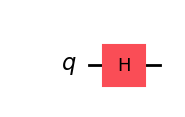
\includegraphics[width=0.3\textwidth]{Images/hadamard.png}
    \caption{Hadamard Gate}
    \label{fig:hadamard}
\end{figure}
In the operator Notation it is:
\begin{align*}
    H\ket{0}&=\dfrac{1}{\sqrt{2}}(\ket{0}+\ket{1})=\ket{+} \\
    H\ket{1}&=\dfrac{1}{\sqrt{2}}(\ket{0}-\ket{1})=\ket{-}
\end{align*}
Generally in a quantum circuit we intialise a qubit in state $\ket{0}$ and thus Hadamard gate can be used
to create a superposition. It is represented by the matrix in the computational basis ($\ket{0},\ket{1}$) as:
\[
    H=\dfrac{1}{\sqrt{2}}\begin{bmatrix}
        1 & 1 \\
        1 & -1
    \end{bmatrix}
\]
In compact form we can write the action of Hadamard Gate on one qubit as:
\[
    H\ket{j}=\dfrac{1}{\sqrt{2}}\sum_{k=0}^{1}(-1)^{jk}\ket{k}
\]
where $j=0,1$.
It is a Unitary and Hermitian Matrix. It is a Normal Matrix hence Unitarily Diagonalizable. It has eigenvalues, $\lambda_1=1,\lambda_2=-1$ and the corresponding normalized eigenvectors are $\frac{1}{\sqrt{2+\sqrt{2}}}\begin{bmatrix} 1+\frac{1}{\sqrt{2}} \\ \frac{1}{\sqrt{2}}\end{bmatrix}$ and $\frac{1}{\sqrt{2-\sqrt{2}}}\begin{bmatrix} -1 + \frac{1}{\sqrt{2}} \\ \frac{1}{\sqrt{2}}\end{bmatrix}$ respectively.
It has a Spectral decomposition (outer product representation) which can be written as:
\[
    H=\ket{+}\bra{0}+\ket{-}\bra{1}
\]
Action of Hadamard Gate on a general qubit $\ket{\psi}=\alpha\ket{0}+\beta\ket{1}$ is:
\[
    \dfrac{1}{\sqrt{2}}\begin{bmatrix}
        1 & 1 \\
        1 & -1
    \end{bmatrix}\begin{bmatrix}
        \alpha \\
        \beta
    \end{bmatrix}=\begin{bmatrix}
        \dfrac{\alpha+\beta}{\sqrt{2}} \\
        \dfrac{\alpha-\beta}{\sqrt{2}}
    \end{bmatrix}=\dfrac{\alpha+\beta}{\sqrt{2}}\ket{0}+\dfrac{\alpha-\beta}{\sqrt{2}}\ket{1}
\]
Note that we cal also write the Hadamard gate as 
\[
H=\frac{X+Z}{\sqrt{2}}=\frac{1}{\sqrt{2}}\left(\begin{bmatrix} 0 & 1 \\ 1 & 0 \end{bmatrix}+\begin{bmatrix} 1 & 0 \\ 0& -1 \end{bmatrix} \right)=\frac{1}{\sqrt{2}}\begin{bmatrix} 1 & 1 \\ 1 & -1 \end{bmatrix}
\]
Note that the Hadamard gate is also a self-inverse gate. Since its Hermitian as well as Unitary, thus $H^{\dagger}=H$ and $H^{\dagger}H=HH^{\dagger}=I; H=H^{-1}$.
Thus, $H^2=I$. Intuitively this means that applying Hadamard gate twice will bring the quantum state back to the same quantum state. This can also be imagined 
as doing rotations on bloch sphere and then arriving back at the same state.
\[ H^2=\dfrac{1}{\sqrt{2}}\begin{bmatrix}
    1 & 1 \\
    1 & -1
\end{bmatrix}\dfrac{1}{\sqrt{2}}\begin{bmatrix}
    1 & 1 \\
    1 & -1
\end{bmatrix}=\dfrac{1}{2}\begin{bmatrix}
    1+1 & 1-1 \\
    1-1 & 1+1
\end{bmatrix}=\begin{bmatrix}
    1 & 0 \\
    0 & 1
\end{bmatrix}=I
\]
Thus, we can see that the Hadamard gate is self-inverse.
This means that if I apply Hadamard gate twice on $\ket{0}$ or on $\ket{1}$ then we will arrive back
at the same state. 
\[ H^2\ket{0}=H\ket{+}=\ket{0} \]
\[ H^2\ket{1}=H\ket{-}=\ket{1} \]

\textbf{Hadamard Gates on Multiple Qubits}\\
Hadamard gate can also be applied on multiple qubits. The Hadamard gate on multiple qubits (say n qubits) using tensor products is given as:
\[
    H^{\otimes n}=\underbrace{H\otimes H\otimes \ldots \otimes H}_{n \text{ times}}
\]
One of the way to find the Hadamard matrix is to perform the tensor product n times to get the Hadamard matrix acting on the n qubits. For example, we can find Hadamard gate acting on 2 qubits in matrix form using tensor product as:
\[
    H^{\otimes 2}=\dfrac{1}{\sqrt{2}}\begin{bmatrix}
        1 & 1 \\
        1 & -1
    \end{bmatrix}\otimes \dfrac{1}{\sqrt{2}}\begin{bmatrix}
        1 & 1 \\
        1 & -1
    \end{bmatrix}=\dfrac{1}{2}\begin{bmatrix}
        1 & 1 & 1 & 1 \\
        1 & -1 & 1 & -1 \\
        1 & 1 & -1 & -1 \\
        1 & -1 & -1 & 1
    \end{bmatrix}
\]
Clearly this does not scale.
Another method is, we can find the action of Hadamard gate on multiple qubits by applying the Hadamard gate on each qubit separately.
\[
    H^{\otimes n}(\ket{0}\otimes \ket{0}\otimes \ldots \otimes \ket{0})=H\ket{0}\otimes H\ket{0}\otimes \ldots \otimes H\ket{0}=\ket{+}\otimes \ket{+}\otimes \ldots \otimes \ket{+}
\]
This is a better method then writing entire matrix for n qubits. Thus, we can see that the Hadamard gate on multiple qubits creates a superposition of all possible states of n qubits.
So, for writing the Hadamard gate on multiple qubits, in a compact form, first we consider the compact form of $H^{\otimes 2}$ as:
\[
H^{\otimes 2}\ket{x}=H\ket{x_1}\otimes H\ket{x_2}
\] 
where $x=x_1x_2$. Now using the fact that $H\ket{x_1}=\dfrac{1}{\sqrt{2}}\sum_{y_1 \in \{0,1\}} (-1)^{x_1y_1}\ket{y_1}$ and $H\ket{x_2}=\dfrac{1}{\sqrt{2}}\sum_{y_2 \in \{0,1\}} (-1)^{x_2y_2}\ket{y_2}$, we get:
\[ 
H^{\otimes 2}\ket{x}=\dfrac{1}{2}\sum_{y_1,y_2 \in \{0,1\}} (-1)^{x_1y_1}(-1)^{x_2y_2}\ket{y_1}\otimes \ket{y_2}=\dfrac{1}{2}\sum_{y \in \{0,1\}^2}(-1)^{x\cdot y}\ket{y}
\]
where $x=x_1x_2$ and $y=y_1y_2$. Thus, it can be generalized and we can write the Hadamard gate on n qubits as:
\[
H^{\otimes n}\ket{x}=\dfrac{1}{\sqrt{2^n}}\sum_{y \in \{0,1\}^n}(-1)^{x\cdot y}\ket{y}
\]
where $x=x_1x_2\ldots x_n$ and $y=y_1y_2\ldots y_n$ and $x\cdot y$ is the dot product between $x$ and $y$. Thus, we can see that the Hadamard gate on n qubits creates a superposition of all possible states of n qubits.
In general, we start with state $\ket{0}$ for all the qubits initially, thus Action of hadamard gate on n qubits all in state $\ket{0}$ is:
\[
    H^{\otimes n}\ket{0}=\dfrac{1}{\sqrt{2^n}}\sum_{y \in \{0,1\}^n}\ket{y}
\]
for Example, explicitly writing $H^{\otimes 2}$, we get,
\[
H^{\otimes 2}=\frac{1}{\sqrt{2^2}}\sum_{x,y}(-1)^{x \cdot y} \ket{x}\bra{y}
\]
\[
=\frac{1}{2} \begin{bmatrix} 1 & 1 & 1 & 1 \\ 1 & -1 & 1 & -1 \\ 1 & 1 & -1 & -1 \\ 1 & -1 & -1 & 1 \end{bmatrix}
\]
Note that here $x,y$ are binary length 2 strings. The sum goes through all pairwise combinations of $x,y \in \{00,01,10,11\}$.
\begin{remark}
    Sylvester's Construction gives an interesting recursive construction of Hadamard matrices. See \href{https://en.wikipedia.org/wiki/Hadamard_matrix}{
https://en.wikipedia.org/wiki/Hadamard\_matrix}. Discussion on interesting (related) open problem concerning the maximal determinant of matrices consisting of entries of $1$ and $-1$ can be found here\\ \href{https://en.wikipedia.org/wiki/Hadamard%27s_maximal_determinant_problem}{https://en.wikipedia.org/wiki/Hadamard\%27s\_maximal\_determinant\_problem}.
\end{remark}
\begin{example}
    \textbf{Fast Hadamard Gate using Tabular method :}\\
    Consider a state 
    \[
    \ket{\psi}=\dfrac{\ket{000}+\ket{110}-\ket{100}-\ket{111}}{\sqrt{4}}
    \]
    We are suppose to find
    $H^{\otimes 3}\ket{\psi}$. Thus, on solving using the equation for hadamard gate acting on multiple qubits $H^{\otimes n}\ket{x}=\dfrac{1}{\sqrt{2^n}}\sum_{y \in \{0,1\}^n}(-1)^{x\cdot y}\ket{y}$ 
    we get,
    \[
        \frac{1}{\sqrt{8}}\left(\ket{001}-\ket{011}+\ket{100}+\ket{110}+\ket{111}\right)
    \]
\end{example}

\subsection{\texorpdfstring{$S$ and $S^{\dagger}$ Gate}{S and S-dagger Gate}}
These are some specialized rotations,
\subsubsection{$S$ Gate}
It is $\pi/2$ rotation around Z axis of Bloch Sphere.
It is also called as the Phase Gate. The truth table is as in table \ref{tab:s}.
\begin{table}[ht]
    \centering
    \begin{tabular}{|c|c|}
        \hline
        Input & Output\\
        \hline
        $\ket{0}$ & $\ket{0}$\\
        $\ket{1}$ & $i\ket{1}$\\
        \hline
    \end{tabular}
    \caption{Truth Table for S Gate}
    \label{tab:s}
\end{table}
The code for the S Gate is as follows:
\begin{lstlisting}[language=Python]
from qiskit import QuantumRegister, ClassicalRegister, QuantumCircuit
from numpy import pi

qreg_q = QuantumRegister(1, 'q')
circuit = QuantumCircuit(qreg_q,name='S Gate')

circuit.s(qreg_q[0]) #Apply the S gate

circuit.draw(output='mpl')#.savefig('../images/s-gate.png') #Draw the circuit
\end{lstlisting}

The circuit symbol is as shown in figure \ref{fig:s}.
\begin{figure}[ht]
    \centering
    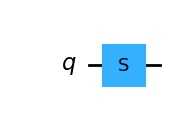
\includegraphics[width=0.3\textwidth]{Images/s-gate.png}
    \caption{S Gate}
    \label{fig:s}
\end{figure}
In the operator Notation it is:
\begin{align*}
    S\ket{0}&=\ket{0} \\
    S\ket{1}&=i\ket{1}
\end{align*}
It is represented by the matrix in the computational basis ($\ket{0},\ket{1}$) as:
\[
    S=\begin{bmatrix}
        1 & 0 \\
        0 & i
    \end{bmatrix}=e^{i\pi/4}\begin{bmatrix}
        e^{-i\pi/4} & 0 \\
        0 & e^{i\pi/4}
    \end{bmatrix}
\]
Thus, it is called as $\pi/4$ gate.
It's Eigen values are 1 and $i$. It's corresponding Eigen vectors are $\ket{0}$ and $\ket{1}$.
It is a Unitary and Hermitian Matrix. It is a Normal Matrix hence Unitarily Diagonalizable.
It has a Spectral decomposition (outer product representation) which can be written as:
\[
    S=\ket{0}\bra{0}+i\ket{1}\bra{1}
\]
Action of S Gate on a general qubit $\ket{\psi}=\alpha\ket{0}+\beta\ket{1}$ is:
\[
    \begin{bmatrix}
        1 & 0 \\
        0 & i
    \end{bmatrix}\begin{bmatrix}
        \alpha \\
        \beta
    \end{bmatrix}=\begin{bmatrix}
        \alpha \\
        i\beta
    \end{bmatrix}=\alpha\ket{0}+i\beta\ket{1}
\]


\subsubsection{$S^{\dagger}$ Gate}
It is $\pi/2$ rotation around Z axis of Bloch Sphere in the opposite direction.
It is also
called as the Conjugate Phase Gate. The truth table is as in table \ref{tab:s-dagger}.
\begin{table}[ht]
    \centering
    \begin{tabular}{|c|c|}
        \hline
        Input & Output\\
        \hline
        $\ket{0}$ & $\ket{0}$\\
        $\ket{1}$ & $-i\ket{1}$\\
        \hline
    \end{tabular}
    \caption{Truth Table for $S^{\dagger}$ Gate}
    \label{tab:s-dagger}
\end{table}
The code for the $S^{\dagger}$ Gate is as follows:
\begin{lstlisting}[language=Python]
from qiskit import QuantumRegister, ClassicalRegister, QuantumCircuit
from numpy import pi

qreg_q = QuantumRegister(1, 'q')
circuit = QuantumCircuit(qreg_q,name='T Gate')

circuit.sdg(qreg_q[0]) #Apply the sdag gate

circuit.draw(output='mpl')#.savefig('../images/sdag-gate.png') #Draw the circuit
\end{lstlisting}

The circuit symbol is as shown in figure \ref{fig:s-dagger}.
\begin{figure}[ht]
    \centering
    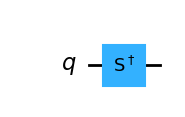
\includegraphics[width=0.3\textwidth]{Images/sdag-gate.png}
    \caption{$S^{\dagger}$ Gate}
    \label{fig:s-dagger}
\end{figure}
In the operator Notation it is:
\begin{align*}
    S^{\dagger}\ket{0}&=\ket{0} \\
    S^{\dagger}\ket{1}&=-i\ket{1}
\end{align*}

It is represented by the matrix in the computational basis ($\ket{0},\ket{1}$) as:
\[
    S^{\dagger}=\begin{bmatrix}
        1 & 0 \\
        0 & -i
    \end{bmatrix}=e^{-i\pi/4}\begin{bmatrix}
        e^{i\pi/4} & 0 \\
        0 & e^{-i\pi/4}
    \end{bmatrix}
\]
It's Eigen values are 1 and $-i$. It's corresponding Eigen vectors are $\ket{0}$ and $\ket{1}$.
It is a Unitary and Hermitian Matrix. It is a Normal Matrix hence Unitarily Diagonalizable.
It has a Spectral decomposition (outer product representation) which can be written as:
\[
    S^{\dagger}=\ket{0}\bra{0}-i\ket{1}\bra{1}
\]
Action of $S^{\dagger}$ Gate on a general qubit $\ket{\psi}=\alpha\ket{0}+\beta\ket{1}$ is:
\[
    \begin{bmatrix}
        1 & 0 \\
        0 & -i
    \end{bmatrix}\begin{bmatrix}
        \alpha \\
        \beta
    \end{bmatrix}=\begin{bmatrix}
        \alpha \\
        -i\beta
    \end{bmatrix}=\alpha\ket{0}-i\beta\ket{1}
\]
\textbf{Note that both $S$ and $S^{\dagger}$ gates are Unitary but not Hermitian thus they are not self-inverse. Recall, that 
the only criteria for a gate is to be a Unitary (from Postulate 2: Unitary evolution) gate and not necessarily Hermitian.}

\subsection{\texorpdfstring{$T$ and $T^{\dagger}$ Gate}{T and T-dagger Gate}}
These are some specialised rotations,
\subsubsection{$T$ Gate}
It is $\pi/4$ rotation around Z axis of Bloch Sphere.
It is also called as the $\pi/8$ Gate. The truth table is as in table \ref{tab:t}.
\begin{table}[ht]
    \centering
    \begin{tabular}{|c|c|}
        \hline
        Input & Output\\
        \hline
        $\ket{0}$ & $\ket{0}$\\
        $\ket{1}$ & $e^{i\pi/4}\ket{1}$\\
        \hline
    \end{tabular}
    \caption{Truth Table for T Gate}
    \label{tab:t}
\end{table}

The code for the T Gate is as follows:
\begin{lstlisting}[language=Python]
from qiskit import QuantumRegister, ClassicalRegister, QuantumCircuit
from numpy import pi

qreg_q = QuantumRegister(1, 'q')
circuit = QuantumCircuit(qreg_q,name='T Gate')

circuit.sdg(qreg_q[0]) #Apply the T gate

circuit.draw(output='mpl')#.savefig('../images/sdag-gate.png') #Draw the circuit    
\end{lstlisting}

The circuit symbol is as shown in figure \ref{fig:t}.
\begin{figure}[ht]
    \centering
    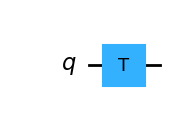
\includegraphics[width=0.3\textwidth]{Images/t-gate.png}
    \caption{T Gate}
    \label{fig:t}
\end{figure}

In the operator Notation it is:
\begin{align*}
    T\ket{0}&=\ket{0} \\
    T\ket{1}&=e^{i\pi/4}\ket{1}
\end{align*}
It is represented by the matrix in the computational basis ($\ket{0},\ket{1}$) as:
\[
    T=\begin{bmatrix}
        1 & 0 \\
        0 & e^{i\pi/4}
    \end{bmatrix}=e^{i\pi/8}\begin{bmatrix}
        e^{-i\pi/8} & 0 \\
        0 & e^{i\pi/8}
    \end{bmatrix}
\]
Thus, it is called as $\pi/8$ gate. This is because up to an unimportant global phase $T$ is equal to a gate which has $e^{\pm \iota \phi/8}$ appearing on its diagonals.
It's Eigen values are 1 and $e^{i\pi/4}$. It's corresponding Eigen vectors are $\ket{0}$ and $\ket{1}$.
It is a Unitary and Hermitian Matrix. It is a Normal Matrix hence Unitarily Diagonalizable.
It has a Spectral decomposition (outer product representation) which can be written as:
\[
    T=\ket{0}\bra{0}+e^{i\pi/4}\ket{1}\bra{1}
\]
Action of T Gate on a general qubit $\ket{\psi}=\alpha\ket{0}+\beta\ket{1}$ is:
\[
    \begin{bmatrix}
        1 & 0 \\
        0 & e^{i\pi/4}
    \end{bmatrix}\begin{bmatrix}
        \alpha \\
        \beta
    \end{bmatrix}=\begin{bmatrix}
        \alpha \\
        e^{i\pi/4}\beta
    \end{bmatrix}=\alpha\ket{0}+e^{i\pi/4}\beta\ket{1}
\]

\subsubsection{$T^{\dagger}$ Gate}
It is $\pi/4$ rotation around Z axis of Bloch Sphere in the opposite direction.
It is also called as the $\pi/8$ Gate. The truth table is as in table \ref{tab:t-dagger}.
\begin{table}[ht]
    \centering
    \begin{tabular}{|c|c|}
        \hline
        Input & Output\\
        \hline
        $\ket{0}$ & $\ket{0}$\\
        $\ket{1}$ & $e^{-i\pi/4}\ket{1}$\\
        \hline
    \end{tabular}
    \caption{Truth Table for $T^{\dagger}$ Gate}
    \label{tab:t-dagger}
\end{table}

The code for the $T^{\dagger}$ Gate is as follows:
\begin{lstlisting}[language=Python]
from qiskit import QuantumRegister, ClassicalRegister, QuantumCircuit
from numpy import pi

qreg_q = QuantumRegister(1, 'q')
circuit = QuantumCircuit(qreg_q,name='T Gate')

circuit.tdg(qreg_q[0]) #Apply the T gate

circuit.draw(output='mpl')#.savefig('../images/tdag-gate.png') #Draw the circuit
\end{lstlisting}

The circuit symbol is as shown in figure \ref{fig:t-dagger}.
\begin{figure}[ht]
    \centering
    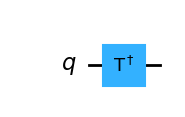
\includegraphics[width=0.3\textwidth]{Images/tdag-gate.png}
    \caption{$T^{\dagger}$ Gate}
    \label{fig:t-dagger}
\end{figure}

In the operator Notation it is:
\begin{align*}
    T^{\dagger}\ket{0}&=\ket{0} \\
    T^{\dagger}\ket{1}&=e^{-i\pi/4}\ket{1}
\end{align*}

One might wonder why the T gate is called the $\pi/8$ gate when it is $\pi/4$ that appears in the definition. The reason is that the gate has historically often been referred to as the $\pi/8$ gate simply because up to an unimportant global phase $T$ is equal to a gate which has $exp(\pm \iota \pi/8)$ appearing on its diagonals. It is represented by the matrix in the computational basis ($\ket{0},\ket{1}$) as:
\[
    T^{\dagger}=\begin{bmatrix}
        1 & 0 \\
        0 & e^{-i\pi/4}
    \end{bmatrix}=e^{-i\pi/8}\begin{bmatrix}
        e^{i\pi/8} & 0 \\
        0 & e^{-i\pi/8}
    \end{bmatrix}
\]
It's Eigen values are 1 and $e^{-i\pi/4}$. It's corresponding Eigen vectors are $\ket{0}$ and $\ket{1}$.
It is a Unitary and Hermitian Matrix. It is a Normal Matrix hence Unitarily Diagonalizable.
It has a Spectral decomposition (outer product representation) which can be written as:
\[
    T^{\dagger}=\ket{0}\bra{0}+e^{-i\pi/4}\ket{1}\bra{1}
\]
Action of $T^{\dagger}$ Gate on a general qubit $\ket{\psi}=\alpha\ket{0}+\beta\ket{1}$ is:
\[
    \begin{bmatrix}
        1 & 0 \\
        0 & e^{-i\pi/4}
    \end{bmatrix}\begin{bmatrix}
        \alpha \\
        \beta
    \end{bmatrix}=\begin{bmatrix}
        \alpha \\
        e^{-i\pi/4}\beta
    \end{bmatrix}=\alpha\ket{0}+e^{-i\pi/4}\beta\ket{1}
\]

Some relations between S and T Gates:
\begin{align*}
    S&=T^2 \\
    S^{\dagger}&=T^{\dagger}T^{\dagger}
\end{align*}
This can be verified as follows. Intuitively, one can think as twice $\pi/4$
rotation around Z axis is $\pi/2$ rotation around Z axis. Thus, the reltaions.
\begin{align*}
    T^2&=\begin{bmatrix}
        1 & 0 \\
        0 & e^{i\pi/4}
    \end{bmatrix}\begin{bmatrix}
        1 & 0 \\
        0 & e^{i\pi/4}
    \end{bmatrix}=\begin{bmatrix}
        1 & 0 \\
        0 & e^{i\pi/2}
    \end{bmatrix}=\begin{bmatrix}
        1 & 0 \\
        0 & i
    \end{bmatrix}=S \\
    T^{\dagger}T^{\dagger}&=\begin{bmatrix}
        1 & 0 \\
        0 & e^{-i\pi/4}
    \end{bmatrix}\begin{bmatrix}
        1 & 0 \\
        0 & e^{-i\pi/4}
    \end{bmatrix}=\begin{bmatrix}
        1 & 0 \\
        0 & e^{-i\pi/2}
    \end{bmatrix}=\begin{bmatrix}
        1 & 0 \\
        0 & -i
    \end{bmatrix}=S^{\dagger}
\end{align*}
\begin{example}
Let $x$ be a real number and $A$ a matrix such that $A^2=I$. Show that
\[
exp(\iota Ax)=\cos (x)I + \iota \sin(x) A
\]

Let $\ket{v}$ be an eignevector of $A$ with eigenvalue $\lambda$. It then follows that $A^2\ket{v}=\lambda^2\ket{v}$, and furthermore we have that $A^2 \ket{v}=I\ket{v}=\ket{v}$ by assumption. We obtain that $\lambda^2= 1$ and therefore the only possible eigenvalues of $A$ are $\lambda=\pm 1$. Let $\ket{v_1},\ldots,\ket{v_k}$ be the eigenvectors with eigenvalue $1$ and $\ket{v_{k+1}},\ldots,\ket{v_n}$ be the eigenvectors with eigenvalue $-1$. By the spectral decompositionm, we can write:
\[
A=\sum_{i=1}^k \ket{v_i}\bra{v_i} - \sum_{i=k+1}^n \ket{v_i}\bra{v_i}
\]
so by the definition of operator functions we have:
\[
exp(\iota Ax)=\sum_{i=1}^k exp(\iota x)\ket{v_i}\bra{v_i} + \sum_{i=k+1}^n exp(-\iota x) \ket{v_i}\bra{v_i}
\]
By Euler's identity we have:
\[
exp(\iota Ax)=\sum_{i=1}^k (\cos(x)+\iota\sin(x))\ket{v_i}\bra{v_i} + \sum_{i=k+1}^n (\cos(x)-\iota \sin(x))\ket{v_i}\bra{v_i}
\]
Grouping terms, we obtain:
\[
exp(\iota Ax)=\cos(x) \sum_{i=1}^n \ket{v_i}\bra{v_i} + \iota \sin(x)\left(\sum_{i=1}^k \ket{v_i}\bra{v_i}-\sum_{i=k+1}^n \ket{v_1}\bra{v_i}\right)
\]
Using the spectral decomposition and definition of $I$, we therefore obtain the desired relation:
\[
exp(\iota Ax)=\cos(x)I+\iota\sin(x)A
\]
\textbf{Since all of the Pauli matrices satisfy $A^2=I$ i.e they are self inverse, for $\theta\in\mathbb{R}$, we can apply this obtained relation. This will be useful for application in Hamiltonian simulation.}
\end{example}
\begin{example}
    \textbf{Functions of the Pauli matrices} let $\vec{v}$ be any real, three-dimensional unit vector and $\theta$ a real number. Let $f(\cdot)$ be any function from complex numbers to complex numbers. Let $\vec{n}$ be a normalized vector in three dimensions, and let $\theta$ be real. Show that
    \[
    f(\theta \vec{n} \cdot \vec{\sigma})=\frac{f(\theta)+f(-\theta)}{2}I+\frac{f(\theta)-f(-\theta)}{2}\vec{n}\cdot \vec{\sigma}
    \]
    where $\vec{n}\cdot\vec{\sigma}=\sum_{i=1}^3 n_i\cdot\sigma_i$, this implies, $\theta\vec{n}\cdot\vec{\sigma}=\sum_{i=1}^3 \theta n_i\cdot\sigma_i$.
    \begin{align*}
    \sum_{i=1}^3 \theta n_i\sigma_i &= \theta n_1 \ket{+}\bra{+}-\theta n_1\ket{-}\bra{-}+\theta n_2\ket{+\iota}\bra{+\iota}-\theta n_2\ket{-\iota}\bra{-\iota} + \theta n_3\ket{0}\bra{0}-\theta n_3\ket{1}\bra{1}\\
    &=\theta \begin{bmatrix} n_3 & n_1-\iota n_2 \\ n_1 + \iota n_2 & -n_3 \end{bmatrix}
    \end{align*}
    where $\vec{n}$ is a real, three dimensional unit vector and $\theta \in \mathbb{R}$, $n_1,n_2,n_3 \in \mathbb{R}$. Note that the above given matrix is clearly a Hermitian matrix, thus has a unitary decomposition (has complete set of eigenvectors spanning $\mathbb{C}^2$). Now, upon solving for the eigen values we get,
    \[
    \begin{vmatrix} n_3 - \lambda & n-1+\iota n_2  \\ n_1+\iota n_2 & -n_2-\lambda \end{vmatrix} = 0
    \]
    this results in the eigenvalues as (using the property of $\vec{n}$ being a unit vector)
    \[
    \lambda=\pm\sqrt{n_1^2+n_2^2+n_3^2}
    \]
    \[
    \lambda=\pm 1
    \]
    Say it's eigen values are $\ket{v_+}$ corresponding to $\lambda=1$ and $\ket{v_-}$ corresponding to $\lambda=-1$. Thus, we get,
    \[
    \vec{n}\cdot\vec{\sigma}=\ket{v_+}\bra{v_+}-\ket{v_-}\bra{v_-}
    \]
    \[
    \sum_{i=1}^3 \theta n_i\sigma_i=\theta (\ket{v_+}\bra{v_+} - \ket{v_-}\bra{v_-})
    \]
    Now,
    \[
    f(\theta \vec{n}\cdot\vec{\sigma})=f(\theta)\ket{v_+}\bra{v_+}+f(-\theta)\ket{v_-}\bra{v_-}
    \]
    From the completeness relationship, we can write Identity as $I=\ket{v_+}\bra{v_+}+\ket{v_-}\bra{v_-}$, hence, For a observable on a 2-dimensional Hilbert space with eigenvalues$\lambda=\pm 1$ has projectors
    \begin{align*}
    \frac{I+\vec{n}\cdot\vec{\sigma}}{2}&=\ket{v_+}\bra{v_+}\\
    \frac{I-\vec{n}\cdot\vec{\sigma}}{2}&=\ket{v_-}\bra{v_-}
    \end{align*}
    Substituting this in the equation we get,
    \[
    f(\theta\vec{n}\cdot\vec{\sigma})=f(\theta)\frac{I+\vec{n}\cdot\vec{\sigma}}{2}+f(-\theta)\frac{I-\vec{n}\cdot\vec{\sigma}}{2}
    \]
    On simplifying this we get,
    \[
    f(\theta\vec{n}\cdot\vec{\sigma})=\frac{f(\theta)+f(-\theta)}{2}I+\frac{f(\theta)-f(-\theta)}{2}\vec{n}\cdot\vec{\sigma}
    \]
    In case we write the function as $exp(\iota \theta\vec{n}\cdot\vec{\sigma})$ we get,
    \[
    exp(\iota\theta\vec{n}\cdot\vec{\sigma})=\cos(\theta)I+\iota\sin(\theta) \vec{n}\cdot\vec{\sigma}
    \]
    \end{example}


\subsection{Quantum Rotation Gates}
These are generalized rotations  in the Bloch Sphere 
denoted as $R_X,R_Y,R_Z$ about the X,Y and Z axis of Bloch Sphere respectively. The Pauli matrices give rise to three useful classes of Unitary matrices when they are exponentiated, the rotation operators about the $x,y,z$ axes.
\subsubsection{$R_X$ Gate}
It is a rotation about X axis of Bloch Sphere by an angle $\theta$. Putting $\vec{n}=(1,0,0)$ in the previous equation and putting $\theta=-\theta/2$. This is denoted
as $R^{X}_{\theta}$.
The matrix representation of $R^{X}_{\theta}$ is:
\[
    R^{X}_{\theta}=\begin{bmatrix}
        \cos(\theta/2) & -i\sin(\theta/2) \\
        -i\sin(\theta/2) & \cos(\theta/2)
    \end{bmatrix}=\cos \frac{\theta}{2}I-\iota \sin\frac{\theta}{2}\sigma_X=e^{-\iota\frac{\theta}{2}\sigma_X}
\]
The code for the $R_X$ Gate is as follows:
\begin{lstlisting}[language=Python]
from qiskit import QuantumRegister, ClassicalRegister, QuantumCircuit
from numpy import pi

qreg_q = QuantumRegister(1, 'q')
circuit = QuantumCircuit(qreg_q,name='U1 Gate')

circuit.rx(pi/2,qreg_q[0]) #Apply the RX gate

circuit.draw(output='mpl')#.savefig('../images/rx-gate.png') #Draw the circuit
\end{lstlisting}

The circuit symbol is as shown in figure \ref{fig:rx}.
\begin{figure}[ht]
    \centering
    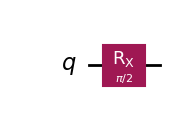
\includegraphics[width=0.3\textwidth]{Images/rx-gate.png}
    \caption{$R_X$ Gate}
    \label{fig:rx}
\end{figure}
Note that the value $\pi/2$ given in the figure \ref{fig:rx} denotes the angle by which we rotate around the X Axis of Bloch Sphere. Note that $R_{\pi}^{X} = -\iota X$.

\subsubsection{$R_Y$ Gate}
It is a rotation about Y axis of Bloch Sphere by an angle $\theta$. This is denoted
as $R^{Y}_{\theta}$.
The matrix representation of $R^{Y}_{\theta}$ is:
\[
    R^{Y}_{\theta}=\begin{bmatrix}
        \cos(\theta/2) & -\sin(\theta/2) \\
        \sin(\theta/2) & \cos(\theta/2)
    \end{bmatrix}= \cos \frac{\theta}{2}I-\iota \sin \frac{\theta}{2}\sigma_Y=e^{-\iota \frac{\theta}{2}\sigma_Y}
\]
The code for the $R_Y$ Gate is as follows:
\begin{lstlisting}[language=Python]
from qiskit import QuantumRegister, ClassicalRegister, QuantumCircuit
from numpy import pi

qreg_q = QuantumRegister(1, 'q')
circuit = QuantumCircuit(qreg_q,name='RY Gate')

circuit.ry(pi/2,qreg_q[0]) #Apply the RY gate

circuit.draw(output='mpl')#.savefig('../images/ry-gate.png') #Draw the circuit
\end{lstlisting}

The circuit symbol is as shown in figure \ref{fig:ry}.
\begin{figure}[ht]
    \centering
    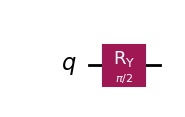
\includegraphics[width=0.3\textwidth]{Images/ry-gate.png}
    \caption{$R_Y$ Gate}
    \label{fig:ry}
\end{figure}
Note here the value $\pi/2$ denotes the angle by which we rotate around the Y Axis of Bloch Sphere. Note that $R_{\pi}^Y=-\iota Y$.

\subsubsection{$R_Z$ Gate}
It is a rotation about Z axis of Bloch Sphere by an angle $\theta$. This is denoted
as $R^{Z}_{\theta}$.
The matrix representation of $R^{Z}_{\theta}$ is:
\[
    R^{Z}_{\theta}=\begin{bmatrix}
        e^{-i\theta/2} & 0 \\
        0 & e^{i\theta/2}
    \end{bmatrix}=\cos \frac{\theta}{2}I-\iota \sin \frac{\theta}{2}\sigma_Z=e^{-\iota \frac{\theta}{2}\sigma_Z}
\]

The code for the $R_Z$ Gate is as follows:
\begin{lstlisting}[language=Python]
from qiskit import QuantumRegister, ClassicalRegister, QuantumCircuit
from numpy import pi

qreg_q = QuantumRegister(1, 'q')
circuit = QuantumCircuit(qreg_q,name='RZ Gate')

circuit.rz(pi/2,qreg_q[0]) #Apply the RZ gate

circuit.draw(output='mpl')#.savefig('../images/rz-gate.png') #Draw the circuit
\end{lstlisting}

The circuit symbol is as shown in figure \ref{fig:rz}.
\begin{figure}[ht]
    \centering
    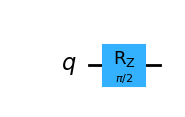
\includegraphics[width=0.3\textwidth]{Images/rz-gate.png}
    \caption{$R_Z$ Gate}
    \label{fig:rz}
\end{figure}
Note here the value $\pi/2$ denotes the angle by which we rotate around the Z Axis of Bloch Sphere. Note that $R_{\pi}^Z = -\iota Z$.

This Quantum Rotation Gates can be used in making variational circuit as angles can vary.

\subsubsection{$R_n$ \textbf{Gate}}
If $\hat{n}=(n_x,n_y,n_z)$ is a real unit vector in three dimensions then we generalize the previous definitions by defining a rotation by $\theta$ about the $\hat{n}$ axis by the equation
\[
R_{\hat{n}}(\theta)=exp(-\iota \theta \hat{n}\cdot \vec{\sigma}/2)=\cos \left(\frac{\theta}{2}\right)I- \iota \sin \left(\frac{\theta}{2}\right) (n_xX+n_yY+n_zZ)
\]
where $\vec{\sigma}$ denotes the three component vector $(X,Y,Z)$ of Pauli matrices. Thus, in matrix form, we can write $R_n(\theta)$ as:
\[
\begin{bmatrix} \cos \frac{\theta}{2} - \iota \sin \frac{\theta}{2} n_z & -\sin \frac{\theta}{2} (n_y+\iota n_x)\\ \sin \frac{\theta}{2} (n_y-\iota n_x) & \cos\frac{\theta}{2} + \iota \sin \frac{\theta}{2} n_z \end{bmatrix}
\]
\subsection{Universal Quantum Gates}
To construct any single qubit Quantum gates.
\[
    U_3(\theta,\phi,\lambda)=\begin{bmatrix}
        \cos(\theta/2) & -e^{i\lambda}\sin(\theta/2) \\
        e^{i\phi}\sin(\theta/2) & e^{i(\phi+\lambda)}\cos(\theta/2)
    \end{bmatrix}
\]
where $\theta,\phi,\lambda\in\mathbb{R}$ are rotations around x, y and z axis respectively.
Here, $0 \leq \theta \leq \pi$, $0\leq \phi \leq 2\pi$ and $0\leq \lambda \leq 2\pi$.
Similarly, we can fix $\theta$ and write $U_2$ gate as:
\[
    U_2(\phi,\lambda)=\begin{bmatrix}
        1 & -e^{i\lambda} \\
        e^{i\phi} & e^{i(\phi+\lambda)}
    \end{bmatrix}
\]
Here $\theta=\pi/2$ by default.
Similarly, we can fix $\theta$ and $\phi$ and write $U_1$ gate as:
\[
    U_1(\lambda)=\begin{bmatrix}
        1 & 0 \\
        0 & e^{i\lambda}
    \end{bmatrix}
\]
Here $\theta=\phi=0$ by default.

The code for the $U_3$ Gate is as follows:
\begin{lstlisting}[language=Python]
from qiskit import QuantumRegister, ClassicalRegister, QuantumCircuit
from numpy import pi

qreg_q = QuantumRegister(1, 'q')
circuit = QuantumCircuit(qreg_q,name='U3 Gate')

circuit.u(pi/2,pi/2,pi/2,qreg_q[0]) #Apply the U3 gate

circuit.draw(output='mpl')#.savefig('../images/u3-gate.png') #Draw the circuit
\end{lstlisting}

The circuit symbol is as shown in figure \ref{fig:u3}.
\begin{figure}[ht]
    \centering
    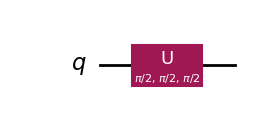
\includegraphics[width=0.3\textwidth]{Images/u3-gate.png}
    \caption{$U_3$ Gate}
    \label{fig:u3}
\end{figure}
Note here the values $\pi/2,\pi/2,\pi/2$ denotes the angles $\theta,\phi,\lambda$ by which we rotate around the Bloch Sphere respectively.

\begin{example}
    Show that, up to a global phase, the $\pi/8$ gate satisfies $T=R_z(\pi/4)$

    Recall that the $T$ gate is defined as:
    \[
    T=\begin{bmatrix} 1 & 0 \\ 0 & exp(\iota \pi/4) \end{bmatrix}
    \]
    We observe that:
    \[
    R_z(\pi/4)=\begin{bmatrix} e^{-\iota \pi/8} & 0 \\ 0 & e^{\iota \pi/8} \end{bmatrix}=e^{-\iota \pi/8}\begin{bmatrix} 1 & 0 \\ 0 & e^{\iota \pi/4} \end{bmatrix} = e^{-\iota \pi/8}T
    \]
\end{example}

\begin{example}
    Express the Hadamard gate $H$ as a product of $R_x$ and $R_z$ rotations and $e^{\iota \varphi}$ for some $\varphi$.

    We claim that $H=R_z(\pi/2)R_x(\pi/2)R_z(\pi/2)$ up to a global phase of $e^{-\iota \pi/2}$. Doing a computation to verify this claim, we see that:
    \begin{align*}
    R_z(\pi/2)R_x(\pi/2)R_z(\pi/2)&=\begin{bmatrix} e^{-\iota \pi/4} & 0 \\ 0 & e^{\iota \pi/4} \end{bmatrix} \begin{bmatrix} \cos(\frac{\pi}{4}) & -\iota \sin(\frac{\pi}{4}) \\ - \iota \sin (\frac{\pi}{4}) & \cos(\frac{\pi}{4}) \end{bmatrix}\begin{bmatrix} e^{-\iota \pi/4} & 0 \\ 0 &e^{\iota \pi/4} \end{bmatrix}\\
    &=\begin{bmatrix} e^{-\iota \pi/4} & 0 \\ 0 & e^{\iota \pi/4} \end{bmatrix} \begin{bmatrix}\frac{1}{\sqrt{2}} & -\frac{\iota}{\sqrt{2}} \\ -\frac{\iota}{\sqrt{2}} & \frac{1}{\sqrt{2}} \end{bmatrix}\begin{bmatrix} e^{-\iota \pi/4} & 0 \\ 0 &e^{\iota \pi/4} \end{bmatrix}\\
    &=\frac{1}{\sqrt{2}} \begin{bmatrix} e^{-\iota \pi/4} & 0 \\ 0 & e^{\iota \pi/4} \end{bmatrix}\begin{bmatrix} e^{-\iota \pi/4} & -\iota e^{\iota\pi/4} \\ -\iota e^{-\iota \pi/4} & e^{\iota \pi/4} \end{bmatrix}\\
    &=\frac{1}{\sqrt{2}}\begin{bmatrix} e^{-\iota \pi/2} & -e^{\iota \pi/2} \\ - e^{-\iota \pi/2} & e^{\iota \pi/2} \end{bmatrix}\\
    &=\frac{e^{-\iota \pi/2}}{\sqrt{2}}\begin{bmatrix} 1 & 1 \\ 1 & -1 \end{bmatrix}\\
    &=e^{-\iota \pi/2} H
    \end{align*}
    Thus, we get,
    \[
    e^{\iota \pi/2} R_z(\pi/2)R_x(\pi/2)R_z(\pi/2) =H
    \]
\end{example}

\begin{example}
    Prove that $(\hat{\mathbf{n}}\cdot \mathbf{\sigma})^2 = I$

    \begin{align*}
    (\hat{\mathbf{n}}\cdot \mathbf{{\sigma}})^2 &= (n_xX+n_yY+n_zZ)^2\\
    &=n_x^2X^2+n_y^2 Y+n_z^2 Z^2 +n_xn_y(XY+YX)+n_xn_z(XZ+ZX)+n_yn_z(YZ+ZY)
    \end{align*}
Recall that $\{\sigma_i,\sigma_j\}=2\delta_{ij}I$, using this, we have that:
\[
(\hat{\mathbf{n}} \cdot \mathbf{\sigma})^2 =(n_z^2 + n_y^2 + n_z^2)I=I
\]
where we use the fact that $\hat{\mathbf{n}}$ is a vector of unit length.
\end{example}

\begin{example}
    One reason why the $\hat{R}_n(\theta)$ operators are referred to as rotation operators is the following fact, which you are to prove. Suppose a single qubit has a state represented by the Bloch vector $\mathbf{\lambda}$. Then, the effects of the rotation $\hat{R}_n(\theta)$ on the state is to rotate by an angle $\theta$ about the $\hat{n}$ axis of the Bloch sphere. This fact explains the rather mysterious looking factors of two in the definition of the rotation matrices.

    Let $\mathbf{\lambda}$ be an arbitrary Bloch vector. Without the loss of generality, we can express $\mathbf{\lambda}$ in a coordinate system such that $\hat{n}$ is aligned with $z$ axis, so it suffices to consider how the state behaves under the application $R_z(\theta)$. Let $\mathbf{\lambda}=()$ be the vector expressed in this coordinate system. We know that the density operator corresponding to this Bloch vector is given by:
    \[
    \rho=\frac{I+\mathbf{\lambda} \cdot \mathbf{\sigma}}{2}
    \]
    We now observe how $\rho$ transforms under the conjugation of $R_z(\theta)$.
    \begin{align*}
        R_z(\theta)\rho R_z(\theta)^{\dagger} &=R_z(\theta)\rho R_z(-\theta)\\
        &=R_z(\theta)\left(\frac{I+\lambda_xX+\lambda_yY+\lambda_zZ}{2}\right)R_z(-\theta)
    \end{align*}
    Using that $XZ=-ZX$, we make the observation that:
    \begin{align*}
        R_z(\theta)X&=\left(\cos \left(\frac{\theta}{2}\right)I-\iota \sin\left(\frac{\theta}{2}\right)Z \right) X\\
        &=X\left(\cos \left(\frac{\theta}{2}\right)I+\iota \sin\left((\frac{\theta}{2}\right)Z\right)\\
        &=X\left(\cos\left(\frac{-\theta}{2}\right)I-\iota \sin\left(\frac{-\theta}{2}\right)Z\right)\\
        &=XR_z(-\theta)
    \end{align*}
    Similarly, we find that $R_z(\theta)Y=YR_z(-\theta)$ (same anticommutation) and that $R_z(\theta)Z=ZR_z(\theta)$ (all terms commute). With this, for expression $R_z(\theta)\rho R_z(\theta)^{\dagger}$ simplifies to:
    \begin{align*}
        R_z(\theta)\rho R_z(\theta)^{\dagger}&=R_z(\theta)\left(\frac{I+\lambda_zX+\lambda_yY+\lambda_zZ}{2}\right) R_z(-\theta)\\
        &= \frac{I+\lambda_xXR_z(-2\theta)+\lambda_yYR_z(-2\theta)+\lambda_zZ}{2}
    \end{align*}
    Calculating each of the terms in the above expression, we have:
    \begin{align*}
        XR_z(-2\theta)&=X\left(\cos\left(\frac{-2\theta}{2}\right)-\iota \sin\left(\frac{-2\theta}{2}\right) Z\right)\\
        &=X(\cos(\theta)+\iota \sin(\theta)Z)\\
        &=\cos(\theta)X+\iota \sin(\theta)XZ\\
        &=\cos(\theta)X+\iota \sin(\theta)(-\iota Y)\\
        &=\cos(\theta)X+\sin(\theta)Y\\
        YR_z(-2\theta)&=Y(\cos(\theta)+\iota \sin(\theta)Z)\\
        &=\cos(\theta)Y+\iota \sin(\theta)YZ\\
        &=\cos(\theta)Y+\iota \sin(theta)(\iota X)\\
        &=\cos(\theta)Y-\sin(\theta)X
    \end{align*}
    Plugging these back into the expression for $R_z(\theta)\rho R_z(\theta)^{\dagger}$ and collecting like terms, we have:
    \[
    R_z(\theta)\rho R_z(\theta)^{\dagger}=\frac{I+(\lambda_x\cos(\theta)-\lambda_y\sin(\theta))X+(\lambda_x\sin(\theta)+\lambda_y\cos(\theta))Y+\lambda_zZ}{2}
    \]
    From this expression, we can read off the new Bloch vector $\mathbf{\lambda'}$ after conjugation by $R_z(\theta)$ to be:
    \[
    \mathbf{\lambda'}=(\lambda_x\cos(\theta)-\lambda_y \sin(\theta),\lambda_x\sin(\theta)+\lambda_y\cos(\theta),\lambda_z)
    \]
    Alternatively, suppose we apply the 3-dimensional rotation matrix $A_z(\theta)$ to the original bloch vector $\mathbf{\lambda}$. We have that:
    \[
    A_z(\theta)\mathbf{\lambda}=\begin{bmatrix}\cos\theta & -\sin\theta & 0 \\ \sin\theta & \cos\theta & 0 \\ 0 & 0 & 1 \end{bmatrix} \begin{bmatrix} \lambda_x \\ \lambda_y \\ \lambda_z \end{bmatrix}=\begin{bmatrix} \lambda_x \cos\theta-\lambda_y \sin\theta \\ \lambda_x\sin\theta+\lambda_y \cos\theta \\ \lambda_z \end{bmatrix}
    \]
    We see that we end up with the same resulting vector $\mathbf{\lambda'}$. We conclude that the conjugation of $\rho$ under $R_z(\theta)$ has the equivalent effect to rotating the Bloch vector by $\theta$ about the z-axis, and hence the effect of $R_n(\theta)$ on one qubit state is to rotate it by an angle $\theta$ about $\hat{\mathbf{n}}$.
    % Alternatively, we can also think of this in a different way as we can write any $\ket{\lambda}= \begin{bmatrix} \cos{\frac{\theta}{2}} \\ e^{\iota \phi}\sin{\frac{\theta}{2}} \end{bmatrix}$ in the $\ket{0},\ket{1}$ basis. Thus, the action of $R_z(\theta)$ on this vector will be
    % \begin{align*}
    % R_z(\theta)\ket{\lambda} &= \cos{\frac{\theta}{2}} \begin{bmatrix} \cos{\frac{\theta}{2}} \\ e^{\iota \phi}\sin{\frac{\theta}{2}} \end{bmatrix} - \iota \sin{\frac{\theta}{2}} \begin{bmatrix} 1 & 0 \\ 0 & -1 \end{bmatrix}\begin{bmatrix} \cos{\frac{\theta}{2}} \\ e^{\iota \phi}\sin{\frac{\theta}{2}} \end{bmatrix}\\
    % &=\begin{bmatrix} e^{-\iota\frac{\theta}{2}} & 0 \\ 0 & e^{\iota \frac{\theta}{2}} \end{bmatrix} \begin{bmatrix} \cos{\frac{\theta}{2}} \\ e^{\iota \phi}\sin{\frac{\theta}{2}} \end{bmatrix}\\
    % &=\begin{bmatrix} e^{-\iota \frac{\theta}{2}}\cos{\frac{\theta}{2}} \\ e^{\iota \phi +\iota \frac{\theta}{2}}\sin{\frac{\theta}{2}} \end{bmatrix}
    % \end{align*}
    % Thus, the state can then be written as $e^{-\iota \frac{\theta}{2}} (\cos(\frac{\theta}{2})\ket{0} + e^{\iota (\phi + \theta)}\sin(\frac{\theta}{2}) \ket{1})$. Ignoring the global phase, we can write this as, $\cos(\frac{\theta}{2})\ket{0} + e^{\iota (\phi + \theta)}\sin(\frac{\theta}{2}) \ket{1}$. Thus, we see that the 

    % Recall that, $R_n(\theta)=\cos(\frac{\theta}{2})I-\iota \sin(\frac{\theta}{2}) (n_x X+n_yY+n_zZ)$, thus we can write $\vec{\lambda} = (\sin{\theta} \cos\phi , \sin \theta \sin \phi, \cos \theta)$.
\end{example}

\begin{example}
    Show that $XYX=-Y$ and use this to prove that $XR_y(\theta)X=R_y(-\theta)$.

    For the first, claim we use that $XY=-YX$ and $X^2=I$ to obtain that
    \[
    XYX=-YXX=-YI=-Y
    \]
    Using this, we have that:
    \begin{align*}
    XR_y(\theta)X&=X\left(\cos\left(\frac{\theta}{2}\right)I-\iota\sin\left(\frac{\theta}{2}\right)Y\right)X\\
    &=\cos\left(\frac{\theta}{2}\right)XIX-\iota \sin\left(\frac{\theta}{2}\right)XYX\\
    &=\cos\left(\frac{\theta}{2}\right) I+\iota \sin\left(\frac{\theta}{2}\right)Y\\
    &=\cos\left(-\frac{\theta}{2}\right)I-\iota \sin\left(-\frac{\theta}{2}\right)Y\\
    &=R_y(-\theta)
    \end{align*}
\end{example}

\begin{example}
    An arbitrary single qubit unitary operator can be written in the form
    \[
    U=exp(\iota \alpha)R_n(\theta)
    \]
    for some real numbers $\alpha$ and $\theta$, and a real three-dimensional unit vector $\hat{n}$.
    \begin{enumerate}
        \item Prove this fact.
        \item Find values for $\alpha$,$\theta$, and $\hat{n}$ giving the Hadamard gate $H$.
        \item Find values for $\alpha,\theta$ and $\hat{n}$ giving the phase gate
        \[
        S=\begin{bmatrix} 1 & 0 \\ 0 & \iota \end{bmatrix}
        \]
    \end{enumerate}
    \begin{enumerate}
        \item By definition, for any unitary operator $U$ we have that $U^{\dagger}U=I$, so for any state vector $\braket{\psi|\psi}=\bra{\psi}U^{\dagger}U\ket{\psi}$. Therefore, all unitary Us are norm-preserving, and hence for a single qubit correspond to some reflection/rotation in 3-dimensional space (up to a global phase factor). Hence, we can write $U=exp(\iota \alpha)R_n(\theta)$ for some $\hat{n}$ (rotation axis), $\theta$ (rotation angle) and $\alpha$(global phase). Any $2\times 2$ unitary matrix for $a^2+b^2+c^2+d^2=1$ can be written as,
        \[
        U=e^{\iota \alpha} \begin{bmatrix} a +\iota b & c+\iota d \\ -c+\iota d & a-\iota b \end{bmatrix}
        \]
        Consider, the given form for $U$. Note that we can write $R_n(\theta)=e^{-\iota \frac{\theta}{2} (n\cdot \sigma)}$ by substituting the values of $X, Y, Z$ pauli matrices and thus arriving at the following matrix as:
        \[
        U=e^{\iota \alpha}\begin{bmatrix} \cos \frac{\theta}{2} - \iota \sin \frac{\theta}{2} n_z & -\sin \frac{\theta}{2} (n_y+\iota n_x)\\ \sin \frac{\theta}{2} (n_y-\iota n_x) & \cos\frac{\theta}{2} + \iota \sin \frac{\theta}{2} n_z \end{bmatrix}
        \]
        As, $n_x^2+n_y^2+n_z^2=1$ this has the same form as the general $U$, also, there are four independent variables- any two of the $n_x,n_y,n_z$ as they are constrained by the equation $n_x^2+n_y^2+n_z^2=1$ and $\theta, \alpha$. hence any arbitrary $2\times 2$ unitary matrix can be written as $U=e^{\iota \alpha}R_n(\theta)$.
        \item Using the fact that $H=\frac{X+Z}{\sqrt{2}}$, and that modulo factor of $\iota$ that $X/Z$ correspond to rotations $R_x(\pi)$ and $R_z(\pi)$, we find that:
        \begin{align*}
            H=\frac{\iota R_x(\pi)+\iota R_z(\pi)}{\sqrt{2}}&=\iota\left(\frac{2\cos{\frac{\pi}{2}}I-\iota \sin\frac{\pi}{2}X-\iota 
            \sin\frac{\pi}{2} Z}{\sqrt{2}}\right)\\
            &=e^{\iota \frac{\pi}{2}} \left(\cos\left(\frac{\pi}{2}\right)I-\iota \sin\left(\frac{\pi}{2}\right)\left(\frac{1}{\sqrt{2}}X+0Y+\frac{1}{\sqrt{2}}Z\right)\right)
        \end{align*}
        Note that in the second equality we use that $\cos\left(\frac{\pi}{2}\right)=0$ and hence $\frac{2}{\sqrt{2}}\cos\left(\frac{\pi}{2}\right)=\cos\left(\frac{\pi}{2}\right)$. From the last expression, we can read off using the definition of $R_n(\theta)$ that $n=\left(\frac{1}{\sqrt{2}},0,\frac{1}{\sqrt{2}}\right)$,$\theta=\pi$, and $\alpha=\frac{\pi}{2}$.
        \item We observe that:
        \[
        R_z\left(\frac{\pi}{2}\right)=\begin{bmatrix} e^{-\iota \pi/4} & 0 \\ 0 & e^{\iota \pi/4} \end{bmatrix}=e^{-\iota \pi/4}\begin{bmatrix} 1 & 0 \\ 0 & \iota \end{bmatrix}
        \]
        Hence:
        \[
        S=e^{\iota \pi/4}R_z\left(\frac{\pi}{2}\right)
        \]
        from which we obtain that $\hat{n}=\hat{z}=(0,0,1),\theta=\frac{\pi}{2}$, and $\alpha=\frac{\pi}{4}$.
    \end{enumerate}
    Note that one can just use the definition:
    \[
    R_n(\theta)=exp(-\iota \theta \hat{n}\cdot \sigma/2)=\cos\left(\frac{\theta}{2}\right)I-\iota \sin\left(\frac{\theta}{2}\right)(n_xX+n_yY+n_zZ)
    \]
    and the fact that $H=(X+Z)/\sqrt{2}$, to arrive at $\cos\left(\frac{\theta}{2}\right)=0,n_x=n_z=\frac{1}{\sqrt{2}},n_y=0$.
\end{example}

An arbitrary unitary operator on a single qubit can be written in many ways as a combination of rotations, together with global phase shifts on the qubit. The following theorem provides a means of expressing an arbitrary single qubit rotation that will be particularly useful in later applications to controlled operations.

\begin{theorem}
    \textbf{(Z-Y decomposition for a single qubit)} Suppose $U$ is a unitary operation on a single qubit. Then there exist a real number $\alpha,\beta,\gamma$ and $\delta$ such that
    \[
    U=e^{\iota \alpha} R_z(\beta)R_y(\gamma)R_z(\delta)
    \]
\end{theorem}
\begin{proof}
    Since $U$ is unitary, the rows and columns of $U$ are orthonormal, from which it follows that there exist real numbers $\alpha,\beta,\gamma,$ and $\delta$ such that
    \[
    U=\begin{bmatrix} e^{\iota (\alpha - \beta/2 -\delta/2)} \cos \frac{\gamma}{2} & -e^{\iota (\alpha-\beta/2+\delta/2}\sin\frac{\gamma}{2}\\
    e^{\iota (\alpha+\beta/2-\delta/2)}\sin\frac{\gamma}{2} & e^{\iota(\alpha+\beta/2+\delta/2}\cos \frac{\gamma}{2} \end{bmatrix}
    \]
    Thus, the equation now follows immediately from the definition of the rotation matrices and matrix multiplication.
\end{proof}
\begin{example}
    Explain why any single qubit unitary operator may be written in the previous form.

    Let $U$ be a single qubit unitary operator. we then have that $U^{\dagger}U=I$, so identifying: 
    \[
    U=\begin{bmatrix} a & b \\ c & d \end{bmatrix} = \begin{bmatrix} \mathbf{v_1} & \mathbf{v_2} \end{bmatrix}
    \]
    we obtain that:
    \[
    \begin{bmatrix} |a|^2 + |c|^2 & a^*b+c^*d \\ ab^*+cd^* & |b|^2+|d|^2 \end{bmatrix} = \begin{bmatrix} 1 & 0 \\ 0 & 1 \end{bmatrix}
    \]
    From the diagonal entries we obtain that $|a|^2+|c|^2=1$ and $|b|^2+|d|^2=1$ and from the off-diagonal entries we obtain that $\braket{v_1,v_2}=0$, and hence the columns of $U$ are orthonormal. From the fact that $|v_1|$ is normalized, we can parametrize the magnitude of the entries with $\gamma \in \mathbb{R}$ such that:
    \[
    |a|=\cos \frac{\gamma}{2}, \quad |c|=\sin \frac{\gamma}{2}
    \]
    from the orthogonality $U^{\dagger}=U^{-1}$ we get, 
    \[
    U^{-1}=\begin{bmatrix} d & -b \\ -c & a \end{bmatrix} =U^{\dagger} = \begin{bmatrix} a^* & c^* \\ b^* & d^* \end{bmatrix}
    \]
    we further obtain that $b=-c^*$ and $d=a^*$, from which we have that $|b|=|c|$ and $|d|=|a|$. Thus, we have the following matrix:
    \[
    U=\begin{bmatrix} a & -c^* \\c & a^* \end{bmatrix}
    \]
    Furthermore, (also from orthogonality) we can parametrize such that for any $arg(a)=-\frac{\beta}{2}-\frac{\delta}{2}$ and $arg(b)=\frac{\beta}{2} - \frac{\delta}{2}$. For $\beta,\delta \in \mathbb{R}$. Finally, multiplying $U$ by a complex phase $e^{\iota \alpha}$ for $\alpha \in \mathbb{R}$ preserves the unitarity of $U$ and the orthonormality of the columns. Combining these facts gives the form as desired.
    We can write,
    \[
    U=\begin{bmatrix} e^{\iota (\alpha - \beta/2 -\delta/2)} \cos \frac{\gamma}{2} & -e^{\iota (\alpha-\beta/2+\delta/2)}\sin\frac{\gamma}{2}\\
    e^{\iota (\alpha+\beta/2-\delta/2)}\sin\frac{\gamma}{2} & e^{\iota(\alpha+\beta/2+\delta/2)}\cos \frac{\gamma}{2} \end{bmatrix}=e^{\iota \alpha} \begin{bmatrix} e^{\iota (- \beta/2 -\delta/2)} \cos \frac{\gamma}{2} & -e^{\iota (-\beta/2+\delta/2)}\sin\frac{\gamma}{2}\\
    e^{\iota (\beta/2-\delta/2)}\sin\frac{\gamma}{2} & e^{\iota(\beta/2+\delta/2)}\cos \frac{\gamma}{2} \end{bmatrix}
    \]
    \[
    =e^{\iota \alpha}\begin{bmatrix} a & -c^* \\ c & a^* \end{bmatrix}
    \]
    which is the general form of a $2\times 2$ unitary matrix as $det(U)=\cos^2 \frac{\gamma}{2} + \sin^2 \frac{\gamma}{2}=1$.
\end{example}
\begin{example}
    \textbf{(X-Y decomposition of rotations)} Give a decomposition analogous to the previous theorem but using $R_x$ instead of $R_z$.

    
We simply use the fact that we can do a change of reference, to interchange the $x$ and $z$ axes. We know that the hadamard $H$ is unitary and self-inverse implements the appropriate swap between $x$ and $z$ axes, while send $y$ to $-y$. So instead of working with $U$ directly, consider
\[
U'=HUH^{-1 }= HUH
\]
which is the frame-rotated $U$. Now, we can use the following ZY decomposition of $U'$.
\[
U'=e^{\iota \alpha}R_z(\beta)R_y(\gamma)R_z(\delta)
\]
What does this imply for $U$? We will see that the above implies an XY-decomposition for $U$.
\begin{align*}
    U=HU'H&=e^{\iota \alpha}(HR_z(\beta)H)(HR_y(\gamma)H)(HR_z(\delta)H)\\
    &=e^{\iota \alpha} R_x(\beta)R_y(-\gamma)R_x(\delta)
\end{align*}
\end{example}
\begin{example}
    Suppose $\hat{m}$ and $\hat{n}$ are non-parallel real unit vectors in three dimensions. Use the theorem to show that an arbitrary single qubit unitary $U$ may be written
    \[
    U=e^{\iota \alpha} R_{\hat{n}}(\beta)R_{\hat{m}}(\gamma)R_{\hat{n}}(\delta)
    \]
    for appropriate choices of $\alpha,\beta,\gamma$ and $\delta$.
    The same arguments in above example could be generalize. We could choose any two orthogonal axes $\hat{n},\hat{m}$ for rotations in our decomposition, using the fact that we can always frame rotate to $z$ and $x$ axes.
\end{example}

Consider the following corollary, which is the key to the construction of controlled multi-qubit unitary operations, as explained.

\begin{corollary}
    Suppose $U$ is a unitary gate on a single qubit. Then there exist unitary operators $A,B,C$ on a single qubit such that $ABC=I$ and $U=e^{\iota \alpha}AXBXC$, where $\alpha$ is some overall phase factor.
\end{corollary}
\begin{proof}
    Set $A=R_z(\beta)R_y(\gamma/2), B=R_y(-\gamma/2)R_z(-(\delta+\beta)/2)$ and $C=R_z((\delta-\beta)/2)$. Note that
    \[
    ABC=R_z(\beta)R_y\left(\frac{\gamma}{2}\right)R_y\left(-\frac{\gamma}{2}\right)R_z\left(-\frac{\delta+\beta}{2}\right)R_z\left(\frac{\delta-\beta}{2}\right)
    \]
    Since $X^2=I$ and $XR_Y(\theta)X=R_y(-\theta)$, we see that,
    \[
    XBX=XR_y\left(-\frac{\gamma}{2}\right)XXR_z\left(-\frac{\delta+\beta}{2}\right)X=R_y\left(\frac{\gamma}{2}\right)R_z\left(\frac{\delta+\beta}{2}\right)
    \]
    Thus
    \begin{align*}
    AXBXC&=R_z(\beta)R_y\left(\frac{\gamma}{2}\right)R_y\left(\frac{\gamma}{2}\right)R_z\left(\frac{\delta+\beta}{2}\right)R_z\left(\frac{\delta-\beta}{2}\right)\\
    &=R_z(\beta)R_y(\gamma)R_z(\delta)
    \end{align*}
    Thus, $U=e^{\iota\alpha}AXBXC$ and $ABC=I$, as required.
\end{proof}

\begin{example}
    Give $A,B,C$ and $\alpha$ for the Hadamard Gate.

    From the proof recall that $U$ is unitary such that
    \[
    U=\begin{bmatrix} e^{\iota (\alpha - \beta/2 -\delta/2)} \cos \frac{\gamma}{2} & -e^{\iota (\alpha-\beta/2+\delta/2)}\sin\frac{\gamma}{2}\\
    e^{\iota (\alpha+\beta/2-\delta/2)}\sin\frac{\gamma}{2} & e^{\iota(\alpha+\beta/2+\delta/2)}\cos \frac{\gamma}{2} \end{bmatrix}
    \]
    This matrix becomes $H$ when $\alpha=\gamma=\frac{\pi}{2},\delta=\pi,\beta=0$. Thus, from the previous corollary, we see that $A=R_z(\beta)R_y(\gamma/2)=R_y\left(\frac{\pi}{4}\right)$, $B=R_y(-\gamma/2)R_z(-(\delta+\beta)/2)=R_y\left(-\frac{\pi}{4}\right)R_z\left(-\frac{\pi}{2}\right)$, $C=R_z((\delta-\beta)/2)=R_z\left(\frac{\pi}{2}\right)$ and $\alpha=0$.
\end{example}

\begin{example}
    \textbf{(Circuit identities)} It is useful to be able to simplify the circuits by inspection, using well-known identities. Prove the following three identities.
    \[
    HXH=Z;\quad HYH=-Y;\quad HZH=X
    \]
    Clearly, 
    \[
    HXH=\frac{1}{2}\begin{bmatrix}1 & 1 \\ 1 & -1 \end{bmatrix}\begin{bmatrix} 0 & 1 \\ 1 & 0 \end{bmatrix}\begin{bmatrix} 1 & 1 \\ 1 & -1 \end{bmatrix} =\frac{1}{2}\begin{bmatrix}2 & 0 \\ 0 & -2 \end{bmatrix} = Z
    \]
    \[
    HYH=\frac{1}{2}\begin{bmatrix} 1 & 1 \\ 1 & -1 \end{bmatrix} \begin{bmatrix} 0 & -\iota \\ \iota & 0 \end{bmatrix} \begin{bmatrix} 1 & 1 \\ 1 & -1 \end{bmatrix} =\frac{1}{2} \begin{bmatrix} 0 & 2\iota \\ -2\iota & 0 \end{bmatrix} =\frac{1}{2}\begin{bmatrix} 0 & 2 \iota \\ -2\iota & 0 \end{bmatrix} = -Y
    \]
    \[
    HZH=HHXHH=X
    \]
\end{example}
\begin{example}
    Use the previous example to show that $HTH=R_x(\pi/4)$, up to a global phase.

    Recall that $T=R_z(\pi/4)$ up to a global phase. Thus, $HTH=HR_z(\pi/4)H$. Thus,
    \[
    HTH=HR_z\left(\frac{\pi}{4}\right)H=H\left(\cos\frac{\pi}{8} I - \iota\sin \frac{\pi}{8}Z\right)H=\cos\frac{\pi}{8} I- \iota\sin\frac{\pi}{8}X=R_x\left(\frac{\pi}{4}\right)
    \]
    \begin{example}
        \textbf{(Composition of single qubit operations)} The Bloch representation gives a nice way to visualize the effect of composing two rotations:
        \begin{enumerate}
            \item Prove that if a rotation through an angle $\beta_1$ about the axis $\hat{n}_1$ is followed by a rotation through an angle $\beta_2$ about an axis $\hat{n}_2$, then the overall rotation is through an angle $\beta_{12}$ about an axis $\hat{n}_{12}$ given by
            \begin{align*}
            c_{12}&=c_1c_2-s_1s_2\hat{n}_1 \cdot \hat{n}_2\\
            s_{12}\hat{n}_{12} &= s_1c_2\hat{n}_1 + c_1s_2\hat{n}_2 +s_1s_2\hat{n}_2 \times \hat{n}_1
            \end{align*}
            \item Show that if $\beta_1=\beta_2$ and $\hat{n}_1=\hat{z}$ these equations simplify to
            \begin{align*}
            c_{12}&=c^2-s^2\hat{z}\cdot\hat{n}_2\\
            s_{12}\hat{n}_{12}&=sc(\hat{z}+\hat{n}_2)-s^2\hat{n}_2\times \hat{z}
            \end{align*}
            where $c=c_1$ and $s=s_1$.
        \end{enumerate}
    \end{example}
    We are required to compute $R_{\hat{n}_2}(\beta_2)R_{\hat{n}_1}(\beta_1)$
    \begin{align*}
        R_{\hat{n}_2}(\beta_2)R_{\hat{n}_1}(\beta_1)&=\left(\cos \frac{\beta_2}{2} I -\iota \sin \frac{\beta_2}{2} \hat{n}_2 \cdot \vec{\sigma}\right) \left(\cos\frac{\beta_1}{2} I -\iota \sin \frac{\beta_1}{2} \hat{n}_1\cdot \vec{\sigma} \right)\\
        &=\cos \frac{\beta_2}{2} \cos \frac{\beta_1}{2} - \iota \cos \frac{\beta_2}{2}\sin\frac{\beta_1}{2} \hat{n}_1\cdot \vec{\sigma} - \iota \sin \frac{\beta_2}{2} \cos \frac{\beta_1}{2} \hat{n}_2\cdot \vec{\sigma} \\
        &\quad -\sin\frac{\beta_2}{2}\sin\frac{\beta_1}{2} (\hat{n}_2\cdot\vec{\sigma})(\hat{n}_1 \cdot\vec{\sigma})\\
        &=[c_2c_1-s_2s_1(\hat{n}_2\cdot\hat{n}_1)]I-\iota [c_1s_2\hat{n}_2+c_2s_1\hat{n}_1+s_2s_1(\hat{n}_2 \times \hat{n}_1)]\cdot\vec{\sigma}
    \end{align*}
    The proof of the identity $(\hat{n}_2 \cdot\vec{\sigma})(\hat{n}_1 \cdot\vec{\sigma})=(\hat{n}_2 \cdot\hat{n}_1)I+\iota (\hat{n}_2\times \hat{n}_1)\cdot \vec{\sigma}$ is as follows:\\
    Recall the familiar Pauli matrix relation already proved in the examples
    \[
    \sigma_i\sigma_j =\delta_{ij} I +\iota \sum_{k=1}^3\epsilon_{ijk}\sigma_k
    \]
    Thus, we can then arrive at the following equation
    \[
    a_i\sigma_ib_j\sigma_j = a_i b_j\delta_{ij} + \iota \sum_{k=1}^3 (a_ib_j\epsilon_{ijk})\sigma_k
    \]
    for $\epsilon_{ijk}=0$ except for $\epsilon_{123}=\epsilon_{231}=\epsilon_{312}=1$, and $\epsilon_{321}=\epsilon_{213}=\epsilon_{132}=-1$. Thus, summing over $i,j=1,2,3$ we get,
    \begin{align*}
    \sum_{i=1}^3\sum_{j=1}^3 a_i\sigma_ib_j\sigma_j &= \sum_{i=1}^3\sum_{j=1}^3a_ib_j \delta_{ij} +\iota \sum_{i=1}^3\sum_{j=1}^3\sum_{k=1}^3(a_ib_j\epsilon_{ijk})\sigma_k\\
    (\hat{a}\cdot\vec{\sigma})(\hat{b}\cdot\vec{\sigma})&=(\hat{a}\cdot\hat{b})I+\iota \sum_{k=1}^3 (\hat{a}\times \hat{b})_k\sigma_k
    \end{align*}
    where $\hat{a}=(a_1,a_2,a_3)$ and $\hat{b}=(b_1,b_2,b_3)$ and $\vec{\sigma} = (X,Y,Z)$. Thus, in the matrix form, we have the following result:
    \[
    (\hat{a}\cdot\vec{\sigma})(\hat{b}\cdot\vec{\sigma})=(\hat{a}\cdot\hat{b})I+\iota (\hat{a}\times \hat{b})\cdot\vec{\sigma}
    \]
    Identifying this operation to a single rotation $R_{\hat{n}_{12}}=c_{12}I-\iota s_{12}\hat{n}_{12}\cdot\vec{\sigma}$, we arrive at the required relations
    \begin{align*}
        c_{12} &=c_1c_2 - s_1s_2 \hat{n}_1\cdot\hat{n}_2\\
        s_{12}\hat{n}_{12} &=s_1c_2\hat{n}_1 + c_1s_2\hat{n}_2 +s_2s_2 \hat{n}_2 \times \hat{n}_1
    \end{align*}
    Setting $\beta_2=\beta_2$ and $\hat{n}_1 = \hat{z}$ in the formulas proven above combined with the fact that $c=c_1=\cos (\beta-1/2)=\cos (\beta_2/2)=c_2$ (and similarly ($s_1=s_2=s$) we have:
    \begin{align*}
        c_{12}&=c^2-s^2 \hat{z}\cdot\hat{n}_2\\
        s_{12}\hat{n}_{12} &=sc\hat{z} + cs\hat{n}_2 -s^2 \hat{n}_2 \times \hat{z} = sc(\hat{z}+\hat{n}_2)-s^2\hat{n}_2 \times \hat{z}
    \end{align*}
\end{example}
\section{Multi-Qubit Gates}
If $A$ is true, then do $B$. This type of controlled operation is one of the most useful in computing, both classical and quantum.  We will now see how complex controlled operations are implemented using quantum circuits built from elementary operations.
Quantum Pauli gates and hadamard gate are Unitary and Hermitian, and all the other single qubit gate are Unitary, hence, reversible.
In general, we can generalize any single qubit gate to multi-qubit gate.
Note that since all the gates can be in general represented as Unitary Matrices, thus the number of 
qubits in input = number of qubits in output always. Multi-Qubit gates act on multiple qubits at once thus the matrices are of
size $2^n \times 2^n$ where $n$ is the number of qubits.

\subsection{Two-qubit Gates}
\subsubsection{CNOT/CX Gate}
It is a two qubit gate, also called as the Controlled-NOT gate. It has two input qubits, known as the control qubit and the target qubit.
Here the 1st Qubit is controlled and the 2nd Qubit is target.
(It is also possible in the other way that the 2nd Qubit is controlled and the 1st Qubit is target).
This gate is used to create entanglement.
The truth table is as in table \ref{tab:cnot}.
\begin{table}[ht]
    \centering
    \begin{tabular}{|c|c|c|}
        \hline
        Input & Output\\
        \hline
        $\ket{00}$ & $\ket{00}$\\
        $\ket{01}$   & $\ket{01}$\\
        $\ket{10}$   & $\ket{11}$\\
        $\ket{11}$  & $\ket{10}$\\
        \hline
    \end{tabular}
    \caption{Truth Table for CNOT Gate}
    \label{tab:cnot}
\end{table}
For the table in \ref{tab:cnot}, the 1st Qubit is control and the 2nd Qubit is target.
Thus, the CNOT gate flips the target qubit if the control qubit is $\ket{1}$.
The code for the CNOT Gate is as follows:
\begin{lstlisting}[language=Python]
from qiskit import QuantumRegister, ClassicalRegister, QuantumCircuit
from numpy import pi

# Add 2 qubits for CNOT gate demo
qreg_q = QuantumRegister(2, 'q')
circuit = QuantumCircuit(qreg_q,name='CNOT Gate')

circuit.cx(qreg_q[0],qreg_q[1]) #Apply the CNOT gate

circuit.draw(output='mpl')#.savefig('../images/cnot-gate.png') #Draw the circuit
\end{lstlisting}

The circuit symbol is as shown in figure \ref{fig:cnot}.
\begin{figure}[ht]
    \centering
    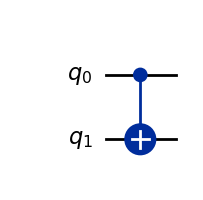
\includegraphics[width=0.3\textwidth]{Images/cnot-gate.png}
    \caption{CNOT Gate}
    \label{fig:cnot}
\end{figure}
Here it can be seen that the 1st Qubit is control and the 2nd Qubit is target. In the
figure \ref{fig:cnot}, the dot denotes the control qubit and the cross denotes the target qubit.

In the operator Notation it is:
\begin{align*}
    CX\ket{00}&=\ket{00} \\
    CX\ket{01}&=\ket{01} \\
    CX\ket{10}&=\ket{11} \\
    CX\ket{11}&=\ket{10}
\end{align*}
It is represented by the matrix in the computational basis ($\ket{00},\ket{01},\ket{10},\ket{11}$) as:
\[
    CX=\begin{bmatrix}
        1 & 0 & 0 & 0 \\
        0 & 1 & 0 & 0 \\
        0 & 0 & 0 & 1 \\
        0 & 0 & 1 & 0
    \end{bmatrix}
\]
In Outer product representation, it can be written as:
\[
    CX=\ket{00}\bra{00}+\ket{01}\bra{01}+\ket{10}\bra{11}+\ket{11}\bra{10}
\]
In Compact form we can write the CNOT gate as:
\[
    CX\ket{x}\ket{y}=\ket{x}\ket{x\oplus y}
\]
where $\oplus$ denotes the XOR operation. If the control qubit is set to $\ket{1}$ then the target qubit is flipped, otherwise the target qubit is left alone. It is a non-linear operation and used in Quantum Error Correction Codes.
This is a very important gate which is used in Teleoprtation protocol, Superdense Coding, Quantum Error Correction Codes etc.
Action of CX/CNOT on general two - qubit $\ket{\psi} = \alpha\ket{00}+\beta\ket{01}+\gamma\ket{10}+\delta\ket{11}$ is:
\[
    \begin{bmatrix} 
        1 & 0 & 0 & 0 \\
        0 & 1 & 0 & 0 \\
        0 & 0 & 0 & 1 \\
        0 & 0 & 1 & 0
    \end{bmatrix}\begin{bmatrix}
        \alpha \\
        \beta \\
        \gamma \\
        \delta
    \end{bmatrix}=\begin{bmatrix}
        \alpha \\
        \beta \\
        \delta \\
        \gamma
    \end{bmatrix}=\alpha\ket{00}+\beta\ket{01}+\delta\ket{10}+\gamma\ket{11}
\]

\subsubsection{CY Gate}
It is a two qubit gate, also called as the Controlled-Y gate.
Here the 1st Qubit is controlled and the 2nd Qubit is target (Pauli - Y Gate)
(It is also possible in the other way that the 2nd Qubit is controlled and the 1st Qubit is target).

The truth table is as in table \ref{tab:cy}.
\begin{table}[ht]
    \centering
    \begin{tabular}{|c|c|c|}
        \hline
        Input & Output\\
        \hline
        $\ket{00}$ & $\ket{00}$\\
        $\ket{01}$   & $\ket{01}$\\
        $\ket{10}$   & $i\ket{10}$\\
        $\ket{11}$  & $-i\ket{11}$\\
        \hline
    \end{tabular}
    \caption{Truth Table for CY Gate}
    \label{tab:cy}
\end{table}
For the table in \ref{tab:cy}, the 1st Qubit is control and the 2nd Qubit is target.
Thus, the CY gate flips the target qubit if the control qubit is $\ket{1}$.
The code for the CY Gate is as follows:
\begin{lstlisting}[language=Python]
from qiskit import QuantumRegister, ClassicalRegister, QuantumCircuit
from numpy import pi

# Add 2 qubits for CNOT gate demo
qreg_q = QuantumRegister(2, 'q')
circuit = QuantumCircuit(qreg_q,name='CY Gate')

circuit.cy(qreg_q[0],qreg_q[1]) #Apply the CY gate

circuit.draw(output='mpl')#.savefig('../images/cy-gate.png') #Draw the circuit
\end{lstlisting}

The circuit symbol is as shown in figure \ref{fig:cy}.
\begin{figure}[ht]
    \centering
    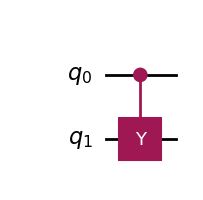
\includegraphics[width=0.3\textwidth]{Images/cy-gate.png}
    \caption{CY Gate}
    \label{fig:cy}
\end{figure}
In this figure \ref{fig:cy}, the first qubit is control and the second qubit is target.
If the first qubit is $\ket{1}$, then Y gate is applied on the second qubit. The Y Gate
is a gate which rotates the qubit by $\pi$ around the Y axis of Bloch Sphere. Thus, if
the input is $\ket{0}$, then the output is $\ket{0}$ and if the input is $\ket{1}$, then the output is $-i\ket{1}$.

In the operator Notation it is:
\begin{align*}
    CY\ket{00}&=\ket{00} \\
    CY\ket{01}&=\ket{01} \\
    CY\ket{10}&=i\ket{11} \\
    CY\ket{11}&=-i\ket{10}
\end{align*}
It is represented by the matrix in the computational basis ($\ket{00},\ket{01},\ket{10},\ket{11}$) as:
\[
    CY=\begin{bmatrix}
        1 & 0 & 0 & 0 \\
        0 & 1 & 0 & 0 \\
        0 & 0 & 0 & -\iota \\
        0 & 0 & \iota & 0
    \end{bmatrix}
\]
In Outer product representation, it can be written as:
\[
    CY=\ket{00}\bra{00}+\ket{01}\bra{01}+\iota\ket{11}\bra{10}-\iota\ket{10}\bra{11}
\]
In Compact form we can write the CY gate as:
\[
    CY\ket{xy}=(-1)^y\iota^x\ket{x(x\oplus y)}
\]
Flipping amplitude of 1 state. Marking of this state can be untilised for marking elements in data base.
It is useful in Grover's Algorithm.

Action of CY on general two - qubit $\ket{\psi} = \alpha\ket{00}+\beta\ket{01}+\gamma\ket{10}+\delta\ket{11}$ is:
\[
    \begin{bmatrix} 
        1 & 0 & 0 & 0 \\
        0 & 1 & 0 & 0 \\
        0 & 0 & 0 & -\iota \\
        0 & 0 & \iota & 0
    \end{bmatrix}\begin{bmatrix}
        \alpha \\
        \beta \\
        \gamma \\
        \delta
    \end{bmatrix}=\begin{bmatrix}
        \alpha \\
        \beta \\
        \iota\delta \\
        -\iota\gamma
    \end{bmatrix}=\alpha\ket{00}+\beta\ket{01}-\iota\delta\ket{10}+\iota\gamma\ket{11}
\]

\subsubsection{CZ/CPHASE Gate}
It is a two qubit gate, also called as the Controlled-Z gate.
Here the 1st Qubit is controlled and the 2nd Qubit is target (Pauli - Z Gate)
(It is also possible in the other way that the 2nd Qubit is controlled and the 1st Qubit is target).

The truth table is as in table \ref{tab:cz}.
\begin{table}[ht]
    \centering
    \begin{tabular}{|c|c|c|}
        \hline
        Input & Output\\
        \hline
        $\ket{00}$ & $\ket{00}$\\
        $\ket{01}$   & $\ket{01}$\\
        $\ket{10}$   & $\ket{10}$\\
        $\ket{11}$  & $-\ket{11}$\\
        \hline
    \end{tabular}
    \caption{Truth Table for CZ Gate}
    \label{tab:cz}
\end{table}
For the table in \ref{tab:cz}, the 1st Qubit is control and the 2nd Qubit is target.
Thus, the CZ gate flips the target qubit if the control qubit is $\ket{1}$.
The code for the CZ Gate is as follows:
\begin{lstlisting}[language=Python]
from qiskit import QuantumRegister, ClassicalRegister, QuantumCircuit
from numpy import pi

qreg_q = QuantumRegister(2, 'q')
circuit = QuantumCircuit(qreg_q,name='CZ Gate')

circuit.cz(qreg_q[0],qreg_q[1]) #Apply the CZ gate

circuit.draw(output='mpl')#.savefig('../images/CZ-gate.png') #Draw the circuit
\end{lstlisting}

The circuit symbol is as shown in figure \ref{fig:cz}.
\begin{figure}[ht]
    \centering
    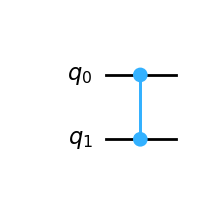
\includegraphics[width=0.3\textwidth]{Images/CZ-gate.png}
    \caption{CZ Gate}
    \label{fig:cz}
\end{figure}
In this figure \ref{fig:cz}, the first qubit is control and the second qubit is target.
If the first qubit is $\ket{1}$, then Z gate is applied on the second qubit. The Z Gate
is a gate which rotates the qubit by $\pi$ around the Z axis of Bloch Sphere. Thus, if 
the input is $\ket{0}$, then the output is $\ket{0}$ and if the input is $\ket{1}$, then the output is $-\ket{1}$.

In the operator Notation it is:
\begin{align*}
    CZ\ket{00}&=\ket{00} \\
    CZ\ket{01}&=\ket{01} \\
    CZ\ket{10}&=\ket{10} \\
    CZ\ket{11}&=-\ket{11}
\end{align*}
It is represented by the matrix in the computational basis ($\ket{00},\ket{01},\ket{10},\ket{11}$) as:
\[
    CZ=\begin{bmatrix}
        1 & 0 & 0 & 0 \\
        0 & 1 & 0 & 0 \\
        0 & 0 & 1 & 0 \\
        0 & 0 & 0 & -1
    \end{bmatrix}
\]
In Outer product representation, it can be written as:
\[
    CZ=\ket{00}\bra{00}+\ket{01}\bra{01}+\ket{10}\bra{10}-\ket{11}\bra{11}
\]
In Compact form we can write the CZ gate as:
\[
    CZ\ket{xy}=(-1)^{xy}\ket{xy}
\]

Action of CZ on general two - qubit $\ket{\psi} = \alpha\ket{00}+\beta\ket{01}+\gamma\ket{10}+\delta\ket{11}$ is:
\[
    \begin{bmatrix} 
        1 & 0 & 0 & 0 \\
        0 & 1 & 0 & 0 \\
        0 & 0 & 1 & 0 \\
        0 & 0 & 0 & -1
    \end{bmatrix}\begin{bmatrix}
        \alpha \\
        \beta \\
        \gamma \\
        \delta
    \end{bmatrix}=\begin{bmatrix}
        \alpha \\
        \beta \\
        \gamma \\
        -\delta
    \end{bmatrix}=\alpha\ket{00}+\beta\ket{01}+\gamma\ket{10}-\delta\ket{11}
\]

\subsubsection{CH/ Controlled Hadamard Gate}
It is a two qubit gate, also called as the Controlled-Hadamard gate.
Here the 1st Qubit is controlled and the 2nd Qubit is target.
The truth table is as in table \ref{tab:ch}.
\begin{table}[ht]
    \centering
    \begin{tabular}{|c|c|c|}
        \hline
        Input & Output\\
        \hline
        $\ket{00}$ & $\ket{00}$\\
        $\ket{01}$   & $\ket{01}$\\
        $\ket{10}$   & $\frac{1}{\sqrt{2}}(\ket{10}+\ket{11})$\\
        $\ket{11}$  & $\frac{1}{\sqrt{2}}(\ket{10}-\ket{11})$\\
        \hline
    \end{tabular}
    \caption{Truth Table for CH Gate}
    \label{tab:ch}
\end{table}
For the table in \ref{tab:ch}, the 1st Qubit is control and the 2nd Qubit is target.
Thus, the CH gate applies Hadamard gate on the target qubit if the control qubit is $\ket{1}$.
The code for the CH Gate is as follows:
\begin{lstlisting}[language=Python]
from qiskit import QuantumRegister, ClassicalRegister, QuantumCircuit
from numpy import pi

# Add 2 qubits for CNOT gate demo
qreg_q = QuantumRegister(2, 'q')
circuit = QuantumCircuit(qreg_q,name='CY Gate')

circuit.ch(qreg_q[0],qreg_q[1]) #Apply the CH gate

circuit.draw(output='mpl')#.savefig('../images/ch-gate.png') #Draw the circuit
\end{lstlisting}

The circuit symbol is as shown in figure \ref{fig:ch}.
\begin{figure}[ht]
    \centering
    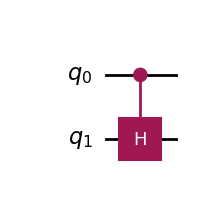
\includegraphics[width=0.3\textwidth]{Images/ch-gate.png}
    \caption{CH Gate}
    \label{fig:ch}
\end{figure}
In this figure \ref{fig:ch}, the first qubit is control and the second qubit is target.
If the first qubit is $\ket{1}$, then Hadamard gate is applied on the second qubit. The Hadamard Gate
is a gate which rotates the qubit by $\pi$ around the X axis of Bloch Sphere. Thus, if
the input is $\ket{0}$, then the output is $\ket{0}$ and if the input is $\ket{1}$, then the output is $\frac{1}{\sqrt{2}}(\ket{0}+\ket{1})$.

In the operator Notation it is:
\begin{align*}
    CH\ket{00}&=\ket{00} \\
    CH\ket{01}&=\ket{01} \\
    CH\ket{10}&=\frac{1}{\sqrt{2}}(\ket{10}+\ket{11}) \\
    CH\ket{11}&=\frac{1}{\sqrt{2}}(\ket{10}-\ket{11})
\end{align*}
It is represented by the matrix in the computational basis ($\ket{00},\ket{01},\ket{10},\ket{11}$) as:
\[
    CH=\begin{bmatrix}
        1 & 0 & 0 & 0 \\
        0 & 1 & 0 & 0 \\
        0 & 0 & \frac{1}{\sqrt{2}} & \frac{1}{\sqrt{2}} \\
        0 & 0 & \frac{1}{\sqrt{2}} & -\frac{1}{\sqrt{2}}
    \end{bmatrix}
\]
In Outer product representation, it can be written as:
\[
    CH=\ket{00}\bra{00}+\ket{01}\bra{01}+\frac{1}{\sqrt{2}}\ket{10}\bra{10}+\frac{1}{\sqrt{2}}\ket{10}\bra{11}
\]
In Compact form we can write the CH gate as:
\[
    CH\ket{xy}=\left(\frac{1}{\sqrt{2}}\right)^x\left(\ket{x(x\oplus y)}+(-1)^y\ket{xy}\right)
\]

Action of CH on general two - qubit $\ket{\psi} = \alpha\ket{00}+\beta\ket{01}+\gamma\ket{10}+\delta\ket{11}$ is:
\[
    \begin{bmatrix} 
        1 & 0 & 0 & 0 \\
        0 & 1 & 0 & 0 \\
        0 & 0 & \frac{1}{\sqrt{2}} & \frac{1}{\sqrt{2}} \\
        0 & 0 & \frac{1}{\sqrt{2}} & -\frac{1}{\sqrt{2}}
    \end{bmatrix}\begin{bmatrix}
        \alpha \\
        \beta \\
        \gamma \\
        \delta
    \end{bmatrix}=\begin{bmatrix}
        \alpha \\
        \beta \\
        \frac{\gamma+\delta}{\sqrt{2}} \\
        \frac{\gamma-\delta}{\sqrt{2}}
    \end{bmatrix}=\alpha\ket{00}+\beta\ket{01}+\frac{\gamma+\delta}{\sqrt{2}}\ket{10}+\frac{\gamma-\delta}{\sqrt{2}}\ket{11}
\]

\begin{importantnote}
    The CX/CNOT, CY, CZ and CH gates are Unitary as well as Hermitian. In, general we can write any of the controlled gates where the first qubit acts as a control bit
    and the second qubit acts as a target bit in matrix form as show:
    \[
        \begin{bmatrix}
            I & 0 \\
            0 & U
        \end{bmatrix}
    \]
    where $I$ is the Identity matrix of size $2(2^{n-1}-1)\times 2(2^{n-1}-1)$ and $U$ is the Unitary matrix of size $2\times 2$. Now for forming any of the n-qubit control gates where 
    there are n-1 control bits and 1 target bit we replace U with the corresponding gate wich we wish to form. 
    For example, for 2-qubit Control Hadamard gate we replace U with the Hadamard gate matrix.
    \[
        \begin{bmatrix}
            I & 0 \\
            0 & H
        \end{bmatrix}
    \]
    Similarly, for any n-qubit control gate we can form the matrix by replacing U with the corresponding gate matrix.
    For example, for 3-qubit control Z gate we replace U with the Z gate matrix.
    \[
        \begin{bmatrix}
            I & 0 \\
            0 & Z
        \end{bmatrix}
    \]
    where I is the Identity matrix of size $6\times 6$ and Z is the Pauli-Z gate matrix of size $2 \times 2$.
    We will later on use this concept to create the CCNOT/Toffoli gate.

    More generally, suppose $U$ is an arbitrary single qubit unitary operation. A controlled-$U$ operation is a two qubit operation, again with a control and a target qubit. If the control qubit is set then $U$ is applied to the target qubit, otherwise the target qubit is left alone; that is, $\ket{c}\ket{t}\rightarrow \ket{c}U^c\ket{t}$. The controlled-$U$ operation is represented by the circuit shown in figure \ref{fig:cu}.
\end{importantnote}
\begin{figure}
        \centering
        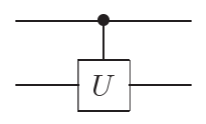
\includegraphics[width=0.25\linewidth]{Images/cu.png}
        \caption{Controlled-$U$ operation. The top line is the control qubit, and the bottom line is the target qubit. If the control qubit is set then $U$ is applied to the target, otherwise it is left alone.}
        \label{fig:cu}
    \end{figure}
\begin{example}
    \textbf{(Matrix representation of multi-qubit gates)}What is the $4\times 4$ unitary matrix for the circuit.
\begin{figure}[ht]
    \centering
    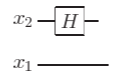
\includegraphics[width=0.25\linewidth]{Images/chexamp.png}
\end{figure}
in the computational basis? What is the unitary matrix for the circuit
\begin{figure}[ht]
    \centering
    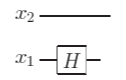
\includegraphics[width=0.25\linewidth]{Images/chexamp2.png}
\end{figure}
    in the computational basis?
Depending upon how the input bits are written as $x_1x_2$ or $x_2x_1$, we can write the matrix in different ways. Say as given in the question we first write $x_1$ and then $x_2$ then the following is the answer:\\
The unitary matrix for the first circuit is given by:
\[
I_1 \otimes H_2 = \begin{bmatrix} 1 & 0 \\ 0 & 1 \end{bmatrix} \otimes \frac{1}{\sqrt{2}}\begin{bmatrix} 1 & 1 \\ 1 & -1 \end{bmatrix} = \frac{1}{\sqrt{2}}\begin{bmatrix} 1 & 1 & 0 & 0 \\ 1 & -1 & 0 & 0 \\ 0 & 0 & 1 & 1 \\ 0 & 0 & 1 & -1 \end{bmatrix}
\]
The unitary matrix for the second circuit is given by:
\[
H_1 \otimes I_2 = \frac{1}{\sqrt{2}}\begin{bmatrix} 1 & 1 \\ 1 & -1 \end{bmatrix}\otimes \begin{bmatrix} 1 & 0 \\ 0 & 1 \end{bmatrix} = \frac{1}{\sqrt{2}} \begin{bmatrix} 1 & 0 & 1 & 0 \\ 0 & 1 & 0 & 1 \\ 1 & 0 & -1 & 0 \\ 0 & 1 & 1 &-1 \end{bmatrix}
\]
\end{example}

\begin{example}
    \textbf{(Building a CNOT from controlled-$Z$ gates)} Construct a CNOT gate from one controlled-$Z$ gate, that is, the gate whose action in the computational basis is specified by the unitary matrix
    \[
    \begin{bmatrix} 1 & 0 & 0 & 0 \\ 0 & 1 & 0 & 0 \\ 0 & 0 & 1 & 0 \\ 0 & 0 & 0 & -1 \end{bmatrix}
    \]
    and two Hadamard gates, specifying the control and target qubits.

    Recall that, $HZH=X$. Hence, to obtain a CNOT gate from a single controlled $Z$ gate, we can conjugate the target qubit with Hadamard gates:
    \begin{figure}[ht]
        \centering
        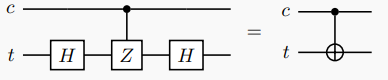
\includegraphics[width=0.5\linewidth]{Images/cnot-z.png}
    \end{figure}
    we can verify this via matrix multiplication, using the result from the previous example:
    \begin{align*}
        (I_1 \otimes H_2)(CZ_{12})(I_1\otimes H_2)&=\frac{1}{2}\begin{bmatrix} 1 & 1 & 0 & 0 \\ 1 & -1 & 0 & 0 \\ 0 & 0 & 1 & 1 \\ 0 & 0 & 1 & -1 \end{bmatrix}\begin{bmatrix} 1 & 0 & 0 & 0\\ 0 & 1 & 0 & 0 \\ 0 & 0 & 1 & 0 \\ 0 & 0 & 0 & -1 \end{bmatrix}\begin{bmatrix} 1 & 1 & 0 & 0 \\ 1 & -1 & 0 & 0 \\ 0 & 0 & 1 & 1 \\ 0 & 0 & 1 & -1 \end{bmatrix}\\
        &=\frac{1}{2}\begin{bmatrix} 2 & 0 & 0 & 0 \\ 0 & 2 & 0 & 0 \\ 0 & 0& 0 &  2\\ 0 & 0 & 2 & 0 \end{bmatrix}\\
        &=CX_{12}
    \end{align*}
\end{example}
\begin{example}
    Show that
    \begin{figure}[ht]
        \centering
        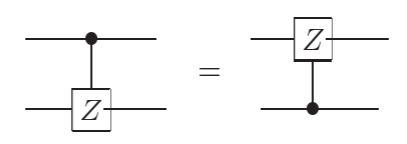
\includegraphics[width=0.5\linewidth]{Images/czzc.png}
    \end{figure}

    Recall that, we can write a controlled-$U$ operation as $CZ\ket{b_1}\ket{b_2} = \ket{b_1}\otimes Z^{b_1}\ket{b_2} = (-1)^{b_1 \cdot b_2} \ket{b_1}\ket{b_2}$ for computational basis states $b_1,b_2\in \{0,1\}$.

    Using this form we can write:
    \begin{align*}
        CZ_{12}\ket{b_1}\ket{b_2} &= (-1)^{b_1\cdot b_2} \ket{b_1}\ket{b_2}\\
        &=(-1)^{b_1\cdot b_2}\ket{b_1}\ket{b_2}\\
        &=Z^{b_2}\ket{b_1}\otimes \ket{b_2}\\
        &=CZ_{21}\ket{b_1}\ket{b_2}
    \end{align*}
    We can also verify this in other ways such as by seeing the action of the controlled gate on all the possible input qubits will be the same.
\end{example}

\begin{example}
    \textbf{(CNOT action on density matrices)} The CNOT gate is a simple permutation whose action on a density matrix $\rho$ is to rearrange the elements in the matrix. Write out this action explicitly in the computational basis.

    Let $\rho$ be an arbitrary density matrix corresponding to a $2$ qubit state. In the computational basis, we can write $\rho$ as:
    \[
    \rho = \begin{bmatrix} a_{11} & a_{12} & a_{12} & a_{14} \\ a_{21} & a_{22} & a_{23} & a_{24} \\ a_{31} & a_{32} & a_{33} & a_{34}\\a_{41} & a-{42} & a_{43} & a_{44} \end{bmatrix}
    \]
    Studying the action of the CNOT gate on this density matrix, we calculate:
    \begin{align*}
        CX_{12}\rho CX_{12} &=\begin{bmatrix} 1 & 0 & 0 & 0 \\ 0 & 1 & 0 & 0 \\ 0 & 0 & 0 & 1 \\ 0 & 0 & 1 & 0 \end{bmatrix} \begin{bmatrix} a_{11} & a_{12} & a_{13} & a_{14} \\ a_{21} & a_{22} & a_{23} & a_{24} \\ a_{31} & a_{32} & a_{33} & a_{34} \\ a_{41} & a_{42} & a_{43} & a_{44} \end{bmatrix}\begin{bmatrix} 1 & 0 & 0 & 0 \\ 0 & 1 & 0 & 0 \\ 0 & 0 & 0 & 1 \\ 0 & 0 & 1 & 0 \end{bmatrix}\\
        &=\begin{bmatrix} a_{11} & a_{12} & a_{13} & a_{14} \\ a_{21} & a_{22} & a_{23} & a_{24} \\ a_{41} & a_{42} & a_{43} & a_{44}\\ a_{31} & a_{32} & a_{33} & a_{34}  \end{bmatrix}\begin{bmatrix} 1 & 0 & 0 & 0 \\ 0 & 1 & 0 & 0 \\ 0 & 0 & 0 & 1 \\ 0 & 0 & 1 & 0 \end{bmatrix}\\
        &=\begin{bmatrix} a_{11} & a_{12} & a_{14} & a_{13}  \\ a_{21} & a_{22} & a_{24} & a_{23}  \\ a_{41} & a_{42}  & a_{44} & a_{43}\\ a_{31} & a_{32} & a_{34} & a_{33}  \end{bmatrix}
    \end{align*}
    Thus, the action of CNOT on density matrices is to rearrange the elements in the matrix as can be seen from the result.
\end{example}

\begin{example}
    \textbf{(CNOT basis transformations)} Unlike ideal classical gates ideal quantum gates do not have (as electrical engineers say)`high impedance' inputs. In fact, the role of `control' and `target' are arbitrary -they depend on what basis you think of a devices as operating in. We have described how CNOT behaves with respect to the computational basis, and in this description the state of the control qubit is not changed. However, if we work in a different basis then the control qubit does change: we will show that its phase is flipped depending on the state of the target qubit! Show that
    \begin{figure}[ht]
        \centering
        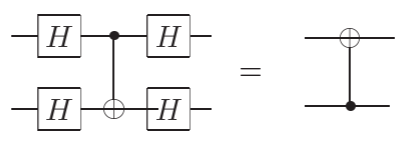
\includegraphics[width=0.5\linewidth]{Images/exampimg.png}
    \end{figure}
    using the identity from the previous example that $CX=(I_1\otimes H_2)(CZ_{12})(I_1\otimes H_2)$, and $CZ_{12}=CZ_{21}$, we get,
    \begin{align*}
        (H\otimes H)(CX_{12})(H\otimes H)&=(H\otimes H)(I\otimes H)(CZ_{12})(I\otimes H)(H\otimes H)\\
        &=(H\otimes I)(CZ_{12})(H\otimes I)\\
        &=(H\otimes I)CZ_{21}(H\otimes I)\\
        &=CX_{21}
    \end{align*}
    which proves the circuit identity. We know already that $CX\ket{c}\ket{t}=\ket{c}\ket{c\oplus t}$. So using the proven identity and the fact that $H\ket{0}=\ket{+},H\ket{1}=\ket{-}$, we obtain the required map.
    Introducing basis states $\ket{\pm} \equiv (\ket{0}\pm\ket{1})/\sqrt{2}$, use this circuit identity to show that the effect of a CNOT with the first qubit as control and the second qubit as target is as follows:
    \begin{align*}
        \ket{+}\ket{+}&\rightarrow \ket{+}\ket{+}\\
        \ket{-}\ket{+}&\rightarrow \ket{-}\ket{+}\\
        \ket{+}\ket{-}&\rightarrow \ket{-}\ket{-}\\
        \ket{-}\ket{-}&\rightarrow \ket{+}\ket{-}
    \end{align*}
    Thus, with respect to this new basis, the state of the target qubit is not changed, while the state of the control qubit is flipped if the target starts as $ket{-}$, otherwise it is left alone. That is, in this basis, the target and control have essentially interchanged roles.
\end{example}
\subsubsection{SWAP Gate}
It is a two Qubit Gate which swaps the states of the two qubits.
The truth table is as in table \ref{tab:swap}.
\begin{table}[ht]
    \centering
    \begin{tabular}{|c|c|c|}
        \hline
        Input & Output\\
        \hline
        $\ket{00}$ & $\ket{00}$\\
        $\ket{01}$   & $\ket{10}$\\
        $\ket{10}$   & $\ket{01}$\\
        $\ket{11}$  & $\ket{11}$\\
        \hline
    \end{tabular}
    \caption{Truth Table for SWAP Gate}
    \label{tab:swap}
\end{table}
The code for the SWAP Gate is as follows:
\begin{lstlisting}[language=Python]
from qiskit import QuantumRegister, ClassicalRegister, QuantumCircuit
from numpy import pi

# Add 2 qubits for CNOT gate demo
qreg_q = QuantumRegister(2, 'q')
circuit = QuantumCircuit(qreg_q,name='SWAP Gate')

circuit.swap(qreg_q[0],qreg_q[1]) #Apply the SWAP gate

circuit.draw(output='mpl')#.savefig('../images/swap-gate.png') #Draw the circuit
\end{lstlisting}

The circuit symbol is as shown in figure \ref{fig:swap}.
\begin{figure}[ht]
    \centering
    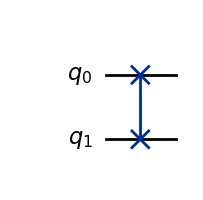
\includegraphics[width=0.3\textwidth]{Images/swap-gate.png}
    \caption{SWAP Gate}
    \label{fig:swap}
\end{figure}

In the operator Notation it is:
\begin{align*}
    SWAP\ket{00}&=\ket{00} \\
    SWAP\ket{01}&=\ket{10} \\
    SWAP\ket{10}&=\ket{01} \\
    SWAP\ket{11}&=\ket{11}
\end{align*}

It is represented by the matrix in the computational basis ($\ket{00},\ket{01},\ket{10},\ket{11}$) as:
\[
    SWAP=\begin{bmatrix}
        1 & 0 & 0 & 0 \\
        0 & 0 & 1 & 0 \\
        0 & 1 & 0 & 0 \\
        0 & 0 & 0 & 1
    \end{bmatrix}
\]
In Outer product representation, it can be written as:
\[
    SWAP=\ket{00}\bra{00}+\ket{01}\bra{10}+\ket{10}\bra{01}+\ket{11}\bra{11}
\]

Action of SWAP on general two - qubit $\ket{\psi} = \alpha\ket{00}+\beta\ket{01}+\gamma\ket{10}+\delta\ket{11}$ is:
\[
    \begin{bmatrix} 
        1 & 0 & 0 & 0 \\
        0 & 0 & 1 & 0 \\
        0 & 1 & 0 & 0 \\
        0 & 0 & 0 & 1
    \end{bmatrix}\begin{bmatrix}
        \alpha \\
        \beta \\
        \gamma \\
        \delta
    \end{bmatrix}=\begin{bmatrix}
        \alpha \\
        \gamma \\
        \beta \\
        \delta
    \end{bmatrix}=\alpha\ket{00}+\gamma\ket{01}+\beta\ket{10}+\delta\ket{11}
\]

SWAP Gate can also be formed using CNOT gates as follows:
\begin{figure}[ht]
    \centering
    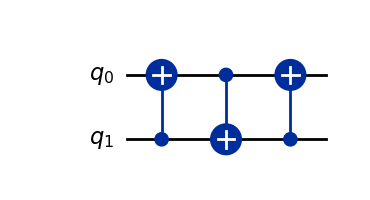
\includegraphics[width=0.3\textwidth]{Images/swap-gatemeth1.png}
    \caption{SWAP Gate using CNOT Gates}
    \label{fig:swap-cnot1}
\end{figure}
Or using CNOT gates as follows:
\begin{figure}[ht]
    \centering
    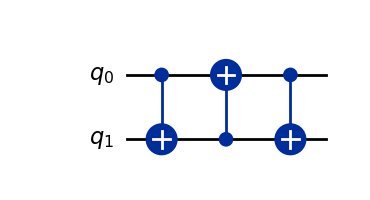
\includegraphics[width=0.3\textwidth]{Images/swap-gatemeth2.png}
    \caption{SWAP Gate using CNOT Gates}
    \label{fig:swap-cnot2}
\end{figure}

\begin{importantnote}
    The global phase does not matter provided we are doing a measurement at the end (or in between). If we are not doing any measurement then the global phase does matter in the computation.
\end{importantnote}



\subsection{Three-qubit Gates}
\subsubsection{CCNOT/Toffoli Gate}
It is a three qubit gate, also called as the CCNOT gate.
Here the 1st and 2nd Qubits are controlled and the 3rd Qubit is target.
The truth table is as in table \ref{tab:toffoli}.
\begin{table}[ht]
    \centering
    \begin{tabular}{|c|c|c|}
        \hline
        Input & Output\\
        \hline
        $\ket{000}$ & $\ket{000}$\\
        $\ket{001}$   & $\ket{001}$\\
        $\ket{010}$   & $\ket{010}$\\
        $\ket{011}$  & $\ket{011}$\\
        $\ket{100}$ & $\ket{100}$\\
        $\ket{101}$   & $\ket{101}$\\
        $\ket{110}$   & $\ket{111}$\\
        $\ket{111}$  & $\ket{110}$\\
        \hline
    \end{tabular}
    \caption{Truth Table for Toffoli Gate}
    \label{tab:toffoli}
\end{table}
For the table in \ref{tab:toffoli}, the 1st and 2nd Qubits are control and the 3rd Qubit is target.
Thus, the Toffoli gate flips the target qubit if the control qubits are $\ket{1}$.
The code for the Toffoli Gate is as follows:
\begin{lstlisting}[language=Python]
from qiskit import QuantumRegister, ClassicalRegister, QuantumCircuit
from numpy import pi

qreg_q = QuantumRegister(3, 'q')
circuit = QuantumCircuit(qreg_q)

circuit.ccx(qreg_q[0], qreg_q[1], qreg_q[2])

circuit.draw(output='mpl')#.savefig('../images/ccx-gate.png')
\end{lstlisting}

The circuit symbol is as shown in figure \ref{fig:toffoli}.
\begin{figure}[ht]
    \centering
    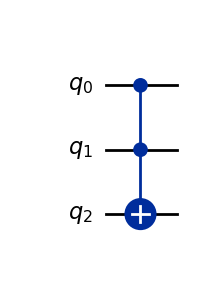
\includegraphics[width=0.3\textwidth]{Images/ccx-gate.png}
    \caption{Toffoli Gate}
    \label{fig:toffoli}
\end{figure}
In this figure \ref{fig:toffoli}, the first and second qubits are control and the third qubit is target.
If the first and second qubits are $\ket{1}$, then the third qubit is flipped. The Toffoli Gate
is a gate which flips the target qubit if the control qubits are $\ket{1}$.

In the operator Notation it is:
\begin{align*}
    CCX\ket{000}&=\ket{000} \\
    CCX\ket{001}&=\ket{001} \\
    CCX\ket{010}&=\ket{010} \\
    CCX\ket{011}&=\ket{011} \\
    CCX\ket{100}&=\ket{100} \\
    CCX\ket{101}&=\ket{101} \\
    CCX\ket{110}&=\ket{111} \\
    CCX\ket{111}&=\ket{110}
\end{align*}

It is represented by the matrix in the computational basis 
($\ket{000},\ket{001},\ldots,\ket{110},\ket{111}$) as:
\[
    CCX=\begin{bmatrix}
        1 & 0 & 0 & 0 & 0 & 0 & 0 & 0 \\
        0 & 1 & 0 & 0 & 0 & 0 & 0 & 0 \\
        0 & 0 & 1 & 0 & 0 & 0 & 0 & 0 \\
        0 & 0 & 0 & 1 & 0 & 0 & 0 & 0 \\
        0 & 0 & 0 & 0 & 1 & 0 & 0 & 0 \\
        0 & 0 & 0 & 0 & 0 & 1 & 0 & 0 \\
        0 & 0 & 0 & 0 & 0 & 0 & 0 & 1 \\
        0 & 0 & 0 & 0 & 0 & 0 & 1 & 0
    \end{bmatrix}
\]
In Outer product representation, it can be written as:
\begin{align*}
    CCX&=\ket{000}\bra{000}+\ket{001}\bra{001}+\ket{010}\bra{010}+\ket{011}\bra{011} \\
    &+\ket{100}\bra{100}+\ket{101}\bra{101}+\ket{110}\bra{111}+\ket{111}\bra{110}
\end{align*}

Action of CCX on general three - qubit $\ket{\psi} = \alpha\ket{000}+\beta\ket{001}+\gamma\ket{010}+\delta\ket{011}+\epsilon\ket{100}+\zeta\ket{101}+\eta\ket{110}+\theta\ket{111}$ is:
\[
    \begin{bmatrix} 
        1 & 0 & 0 & 0 & 0 & 0 & 0 & 0 \\
        0 & 1 & 0 & 0 & 0 & 0 & 0 & 0 \\
        0 & 0 & 1 & 0 & 0 & 0 & 0 & 0 \\
        0 & 0 & 0 & 1 & 0 & 0 & 0 & 0 \\
        0 & 0 & 0 & 0 & 1 & 0 & 0 & 0 \\
        0 & 0 & 0 & 0 & 0 & 1 & 0 & 0 \\
        0 & 0 & 0 & 0 & 0 & 0 & 0 & 1 \\
        0 & 0 & 0 & 0 & 0 & 0 & 1 & 0
    \end{bmatrix}\begin{bmatrix}
        \alpha \\
        \beta \\
        \gamma \\
        \delta \\
        \epsilon \\
        \zeta \\
        \eta \\
        \theta
    \end{bmatrix}=\begin{bmatrix}
        \alpha \\
        \beta \\
        \gamma \\
        \delta \\
        \epsilon \\
        \zeta \\
        \theta \\
        \eta
    \end{bmatrix}=\alpha\ket{000}+\beta\ket{001}+\ldots+\zeta\ket{101}+\theta\ket{110}+\eta\ket{111}
\]

\subsubsection{CSWAP/Fredkin Gate}\label{qgate:cswap}
It is a three qubit gate, also called as the CSWAP gate.
Here the 1st Qubit is control and the 2nd and 3rd Qubits are target.
The truth table is as in table \ref{tab:fredkin}.
\begin{table}[ht]
    \centering
    \begin{tabular}{|c|c|c|}
        \hline
        Input & Output\\
        \hline
        $\ket{000}$ & $\ket{000}$\\
        $\ket{001}$   & $\ket{001}$\\
        $\ket{010}$   & $\ket{010}$\\
        $\ket{011}$  & $\ket{011}$\\
        $\ket{100}$ & $\ket{100}$\\
        $\ket{101}$   & $\ket{110}$\\
        $\ket{110}$   & $\ket{101}$\\
        $\ket{111}$  & $\ket{111}$\\
        \hline
    \end{tabular}
    \caption{Truth Table for Fredkin Gate}
    \label{tab:fredkin}
\end{table}
For the table in \ref{tab:fredkin}, the 1st Qubit is control and the 2nd and 3rd Qubits are target.
Thus, the Fredkin gate swaps the states of the 2nd and 3rd qubits if the control qubit is $\ket{1}$.
The code for the Fredkin Gate is as follows:
\begin{lstlisting}[language=Python]
from qiskit import QuantumRegister, ClassicalRegister, QuantumCircuit
from numpy import pi

qreg_q = QuantumRegister(3, 'q')
circuit = QuantumCircuit(qreg_q)

circuit.cswap(qreg_q[0], qreg_q[2], qreg_q[1])

circuit.draw(output='mpl')#.savefig('../images/cswap-gate.png')
\end{lstlisting}

The circuit symbol is as shown in figure \ref{fig:fredkin}.
\begin{figure}[ht]
    \centering
    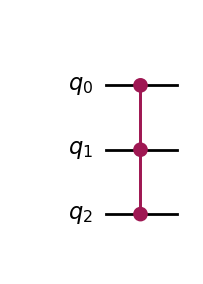
\includegraphics[width=0.3\textwidth]{Images/cswap-gate.png}
    \caption{Fredkin Gate}
    \label{fig:fredkin}
\end{figure}
In this figure \ref{fig:fredkin}, the first qubit is control and the second and third qubits are target.
If the first qubit is $\ket{1}$, then the second and third qubits are swapped. The Fredkin Gate
is a gate which swaps the states of the 2nd and 3rd qubits if the control qubit is $\ket{1}$.

In the operator Notation it is:
\begin{align*}
    CSWAP\ket{000}&=\ket{000} \\
    CSWAP\ket{001}&=\ket{001} \\
    CSWAP\ket{010}&=\ket{010} \\
    CSWAP\ket{011}&=\ket{011} \\
    CSWAP\ket{100}&=\ket{100} \\
    CSWAP\ket{101}&=\ket{110} \\
    CSWAP\ket{110}&=\ket{101} \\
    CSWAP\ket{111}&=\ket{111}
\end{align*}

It is represented by the matrix in the computational basis ($\ket{000},\ket{001},\ldots,\ket{110},\ket{111}$) as:
\[
    CSWAP=\begin{bmatrix}
        1 & 0 & 0 & 0 & 0 & 0 & 0 & 0 \\
        0 & 1 & 0 & 0 & 0 & 0 & 0 & 0 \\
        0 & 0 & 1 & 0 & 0 & 0 & 0 & 0 \\
        0 & 0 & 0 & 1 & 0 & 0 & 0 & 0 \\
        0 & 0 & 0 & 0 & 1 & 0 & 0 & 0 \\
        0 & 0 & 0 & 0 & 0 & 0 & 1 & 0 \\
        0 & 0 & 0 & 0 & 0 & 1 & 0 & 0 \\
        0 & 0 & 0 & 0 & 0 & 0 & 0 & 1
    \end{bmatrix}
\]
In Outer product representation, it can be written as:
\begin{align*}
    CSWAP&=\ket{000}\bra{000}+\ket{001}\bra{001}+\ket{010}\bra{010}+\ket{011}\bra{011} \\
    &+\ket{100}\bra{100}+\ket{101}\bra{110}+\ket{110}\bra{101}+\ket{111}\bra{111}
\end{align*}

Action of CSWAP on general three - qubit $\ket{\psi} = \alpha\ket{000}+\beta\ket{001}+\gamma\ket{010}+\delta\ket{011}+\epsilon\ket{100}+\zeta\ket{101}+\eta\ket{110}+\theta\ket{111}$ is:
\[
    \begin{bmatrix} 
        1 & 0 & 0 & 0 & 0 & 0 & 0 & 0 \\
        0 & 1 & 0 & 0 & 0 & 0 & 0 & 0 \\
        0 & 0 & 1 & 0 & 0 & 0 & 0 & 0 \\
        0 & 0 & 0 & 1 & 0 & 0 & 0 & 0 \\
        0 & 0 & 0 & 0 & 1 & 0 & 0 & 0 \\
        0 & 0 & 0 & 0 & 0 & 0 & 1 & 0 \\
        0 & 0 & 0 & 0 & 0 & 1 & 0 & 0 \\
        0 & 0 & 0 & 0 & 0 & 0 & 0 & 1
    \end{bmatrix}\begin{bmatrix}
        \alpha \\
        \beta \\
        \gamma \\
        \delta \\
        \epsilon \\
        \zeta \\
        \eta \\
        \theta
    \end{bmatrix}=\begin{bmatrix}
        \alpha \\
        \beta \\
        \gamma \\
        \delta \\
        \epsilon \\
        \zeta \\
        \theta \\
        \eta
    \end{bmatrix}=\alpha\ket{000}+\beta\ket{001}+\ldots+\zeta\ket{101}+\theta\ket{110}+\eta\ket{111}
\]

We can construct Fredkin gate using CNOT and Toffoli gate as shown in the figure \ref{fig:fredkin-cnot1}.
\begin{figure}[ht]
    \centering
    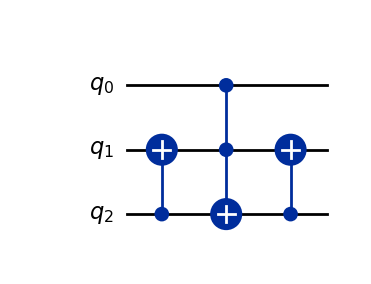
\includegraphics[width=0.3\textwidth]{Images/cswap-gatemeth1.png}
    \caption{Fredkin Gate using CNOT and Toffoli Gates}
    \label{fig:fredkin-cnot1}
\end{figure}

\begin{importantnote}
    Applying a gate on a superposition state is the same as applying the gate on each of the basis states and then superposing the results.
    This is because, the gate is a linear operator and the superposition is a linear combination of the basis states. 
    Thus, the gate can be applied on each of the basis states and then the results can be superposed. For example, Consider a superposition state $\ket{\psi}=\alpha\ket{0}+\beta\ket{1}$.
    If we apply a gate $U$ on this state, then the output will be $U\ket{\psi}=U(\alpha\ket{0}+\beta\ket{1})=\alpha U\ket{0}+\beta U\ket{1}$.
    Thus, the gate can be applied on each of the basis states and then the results can be superposed. This, can also be thought that since U is a $2 \times 2$ matrix and $\ket{0}$ and $\ket{1}$ are $2 \times 1$ column vectors, 
    multiplying $U(\alpha\ket{0}+\ket{1})$ is same as $\alpha U\ket{0}+\beta U\ket{1}$ Since Matrix multiplication is distributive. 

    For example, say CNOT gate needs to be applied on a superposition of two bits $\ket{\psi}=\alpha\ket{00}+\beta\ket{01}+\gamma\ket{10}+\delta\ket{11}$.
    Then the output will be $CNOT\ket{\psi}=CNOT(\frac{\ket{00}+\ket{11}}{\sqrt{2}})=\frac{CNOT\ket{00}+CNOT\ket{11}}{\sqrt{2}}$.
    which will thus be $\frac{\ket{00}+\ket{10}}{\sqrt{2}}$.
    In the matrix form, 
    \[
        CNOT\ket{\psi}=CNOT\left(\frac{\ket{00}+\ket{11}}{\sqrt{2}}\right)=\begin{bmatrix}
            1 & 0 & 0 & 0 \\
            0 & 1 & 0 & 0 \\
            0 & 0 & 0 & 1 \\
            0 & 0 & 1 & 0
        \end{bmatrix}\frac{1}{\sqrt{2}}\left(\begin{bmatrix}
            1 \\
            0 \\
            0 \\
            0
        \end{bmatrix}+\begin{bmatrix}
            0 \\
            0 \\
            0 \\
            1
        \end{bmatrix}\right)
    \]
    \[=\frac{1}{\sqrt{2}}\left(\begin{bmatrix}
        1 & 0 & 0 & 0 \\
        0 & 1 & 0 & 0 \\
        0 & 0 & 0 & 1 \\
        0 & 0 & 1 & 0
    \end{bmatrix}\begin{bmatrix}
        1 \\
        0 \\
        0 \\
        0
    \end{bmatrix}+\begin{bmatrix}
        1 & 0 & 0 & 0 \\
        0 & 1 & 0 & 0 \\
        0 & 0 & 0 & 1 \\
        0 & 0 & 1 & 0
    \end{bmatrix}\begin{bmatrix}
        0 \\
        0 \\
        0 \\
        1
    \end{bmatrix}\right)
    \]
    \[
    =(CNOT\frac{1}{\sqrt{2}}\ket{00}+CNOT\frac{1}{\sqrt{2}}\ket{11})=\frac{1}{\sqrt{2}}CNOT\ket{00}+\frac{1}{\sqrt{2}}CNOT\ket{11}
    \]
    \[
        =\frac{1}{\sqrt{2}}\left(\begin{bmatrix}
            1 \\
            0 \\
            0 \\
            0
        \end{bmatrix}+\begin{bmatrix}
            0 \\
            0 \\
            1 \\
            0
        \end{bmatrix}\right)=\frac{1}{\sqrt{2}}\begin{bmatrix} 1 \\ 0 \\ 1 \\ 0 \end{bmatrix} =\frac{1}{\sqrt{2}}\left(\ket{00}+\ket{10}\right)
    \]
    Thus, applying a gate on a superposition is the same as applying the gate on the basis states of the superposition. Thus, the gate can be applied on each of the basis states and then the results can be superposed
    in the same linear combination as that in which the state $\ket{\psi}$ was superposed.
\end{importantnote}

\section{Implementation of Controlled-U}
Now we are required to understand how to implement the controlled-$U$ operation for arbitrary single qubit $U$, using only single qubit operations and the CNOT gate. Our strategy is a two-part procedure based upon the decomposition $e^{\iota\alpha}AXBXC$.

The first step will be to apply the phase shift exp($\iota\alpha$) on the target qubit, controlled by the control qubit. that is, if the control qubit is $\ket{0}$, then the target qubit is left alone, while if the control qubit is $\ket{1}$, a phase shift $e^{\iota\alpha}$ is applied to the target. A circuit implementing this operation using just a single qubit unitary gate is depicted as in the figure \ref{fig:unicontrolu}. to verify this circuit works correctly, note that the effect of the circuit on the right hand side is
\[
\ket{00}\rightarrow \ket{00},\quad \ket{01}\rightarrow \ket{01},\quad \ket{10}\rightarrow e^{\iota\alpha}\ket{10},\quad \ket{11}\rightarrow e^{\iota\alpha}\ket{11}
\]
\begin{figure}[ht]
    \centering
    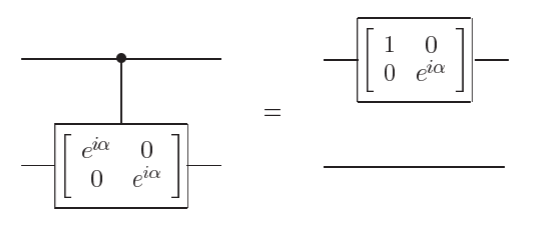
\includegraphics[width=0.5\linewidth]{Images/uncontrolu.png}
    \caption{Controlled phase shift gate and an equivalent circuit for two qubits}
    \label{fig:unicontrolu}
\end{figure}

We can now complete the construction of the controlled-U operation, as shown in figure \ref{fig:univcontrlledu}. to understand why this circuit works, recall that $U$ may be written in the form $U=e^{\iota\alpha}AXBXC$, where $A,B$ and $C$ are single qubit operations such that $ABC=I$. Suppose that the control qubit is set. then the operation $e^{\iota\alpha}AXBXC=U$ is applied to the second qubit. If, on the other hand, the control qubit is not set, then the operation $ABC=I$ is applied to the second qubit; that is, no change is made. That is, the circuit implements the controlled-$U$ operation.
\begin{figure}[ht]
    \centering
    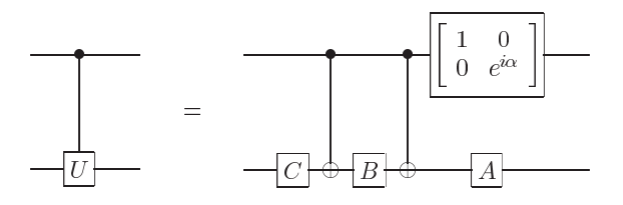
\includegraphics[width=0.5\linewidth]{Images/univcontrolledu.png}
    \caption{Circuit implementing the controlled-U operation for single qubit $U$. $\alpha,A,B$ and $C$ satisfy $U=exp(\iota\alpha) AXBXC, ABC=I$}
    \label{fig:univcontrlledu}
\end{figure}
now that we know how the condition on a single qubit set, what about conditioning on multiple qubits? We've already met one example of multiple qubit conditioning, the Toffoli gate, which flips the third qubit, the target qubit, conditioned on the first two qubits, the control qubits, being set to one. More generally, suppose we have $n+k$ qubits, and $U$ is a $k$ qubit unitary operator. Then we define the controlled operation $C^n(U)$ by the equation.
\[
C^n(U)\ket{x_1x_2\ldots x_n} \ket{\psi} = \ket{x_1x_2\ldots x_n}\ket{\psi}
\]
where $x_1x_2,\ldots x_n$ in the exponent of $U$ means the product of the bits $x_1,x_2,\ldots,x_n$. That is, the operator $U$ is applied to the last $k$ qubits if the first $n$ qubits are equal to one, and otherwise, nothing is done. Such conditional operations are so useful that we introduce a special circuit notation for them, illustrated in figure \ref{fig:multicontrolu}. For the following we assume that $k=1$, for simplicity. larger $k$ can be dealt with using essentially the same methods, however for $k\geq 2$ there is the added complication that we don't know how to perform arbitrary operations on $k$ qubits.
\begin{figure}
    \centering
    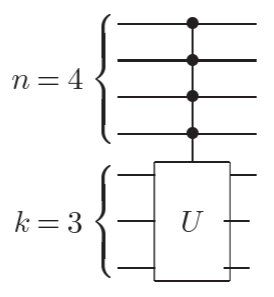
\includegraphics[width=0.25\linewidth]{Images/multicontrolu.png}
    \caption{Sample circuit representation for the $C^n(U)$ operation, where $U$ is a unitary operator on $k$ qubits, for $n=4$ and $k=3$.}
    \label{fig:multicontrolu}
\end{figure}
Suppose $U$ is a single qubit unitary operator, and $V$ is a unitary operator chosen so that $V^2=U$. Then the operation $C^2(U)$ may be implemented using the circuit shown in figure \ref{fig:controlv}.
\begin{figure}
    \centering
    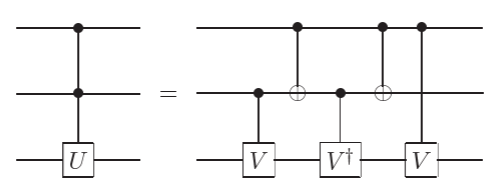
\includegraphics[width=0.75\linewidth]{Images/controlv.png}
    \caption{Circuit for the $C^2(U)$ gate. $V$ is any unitary operator satisfying $V^2=U$. The special case $V\equiv (1-\iota)(I+\iota X)/2$ corresponds to the Toffoli gate.}
    \label{fig:controlv}
\end{figure}
\begin{example}
    Verify that figure \ref{fig:controlv} implements the $C^2(U)$ operation.

    Considering all the possible inputs (in the computational basis) let us see the outcome for both the circuits. 
    \begin{align*}
        \ket{00\psi} &\rightarrow \ket{00\psi}\rightarrow \ket{00\psi}\rightarrow \ket{00\psi}\rightarrow \ket{00\psi}\rightarrow \ket{00\psi}\\
        \ket{01\psi}&\rightarrow \ket{01(V\psi)} \rightarrow \ket{01(V\psi)} \rightarrow \ket{01(V^{\dagger}V\psi)}\rightarrow\ket{01(V^{\dagger}V\psi)}\rightarrow \ket{01(V^{\dagger}V\psi)} = \ket{01\psi}\\
        \ket{10\psi}&\rightarrow \ket{10\psi}\rightarrow \ket{11\psi} \rightarrow \ket{11(V^{\dagger}\psi)} \rightarrow \ket{10(V^{\dagger}\psi)}\rightarrow \ket{10(VV^{\dagger}\psi)} = \ket{10\psi}\\
        \ket{11\psi} &\rightarrow \ket{11(V\psi)} \rightarrow \ket{10(V\psi)} \rightarrow \ket{10(V\psi)} \rightarrow \ket{11(V\psi)} \rightarrow\ket{11(V^2\psi)} = \ket{11(U\psi)}
    \end{align*}
    Hence, the circuit does perform the $C^2(U)$ operation.
\end{example} 

\begin{example}
    Prove that a $C^2(U)$ gate (for any single qubit unitary $U$) can be constructed using at most eight one-qubit gates, and six controlled-NOTs.
    Firstly, we apply the circuit if figure \ref{fig:multicontrolu} to the circuit in figure \ref{fig:controlv} which gives,
    \begin{figure}[ht]
        \centering
        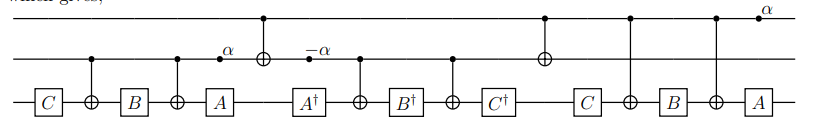
\includegraphics[width=1\linewidth]{Images/c2uimpl.png}
    \end{figure}
    We move the 6th CNOT left from the 4th one, which involves adding CNOTs after the 4th and 5th CNOTs from first to third qubit, which is due to,
    \begin{figure}[ht]
        \centering
        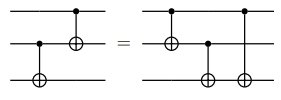
\includegraphics[width=0.5\linewidth]{Images/c2uimpl2.png}
    \end{figure}
    and can be checked by consider all the possible inputs. We also see that $AA^{\dagger}=CC^{\dagger}=I$. Hence, we get the following circuit.
    \begin{figure}[ht]
        \centering
        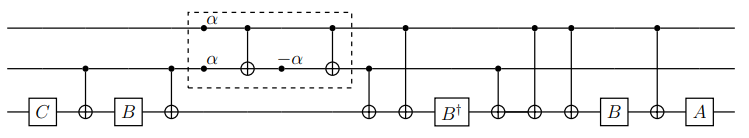
\includegraphics[width=1\linewidth]{Images/c2uimpl3.png}
    \end{figure}
    The dashed is diagonal hence commutes with the rest of the components therefore can be moved to the end for convenience.
    \begin{figure}[ht]
        \centering
        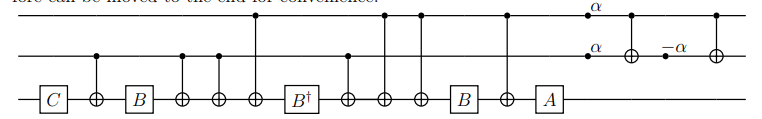
\includegraphics[width=1\linewidth]{Images/c2uimpl4.png}
    \end{figure}
    CNOTs 2 and 3, 6 and 7 cancel each other, hence we are left with the circuit 
    This has $8$ single qubit gates and $6$ CNOTs as desired. The circuit performs the operation, $AXBXB^{\dagger}XBXC=(VC^{\dagger})B^{\dagger}(A^{\dagger}V)=V^2 = U$. Therefore, the circuit performs the $C^2(U)$ operation.
\end{example}

\begin{example} 
Construct a $C^1(U)$ gate for $U=R_x(\theta)$ and $U=R_y(\theta)$, using only CNOT and single qubit gates. Can you reduce the number of single qubit gates need in the construction from three to two?
\end{example}

The familiar Toffoli gate is an especially important special case of $C^2(U)$ operation , the case $C^2(X)$. Defining $V(1-\iota)(I_\iota X)/2$ and noting that $V^2=X$, we see that figure \ref{fig:c2utoff} gives an implementation of the Toffoli gate in terms of one and two qubit operations. From a classical viewpoint this is a remarkable result. Recall that one and two bit classical reversible gates are not sufficient to implement the Toffoli gate, or more generally, universal computation. By contrast, in the quantum case we see that one and two qubit reversible gates are sufficient to implement the Toffoli gate, and will eventually prove that they suffice for universal computation. 
\begin{figure}[ht]
    \centering
    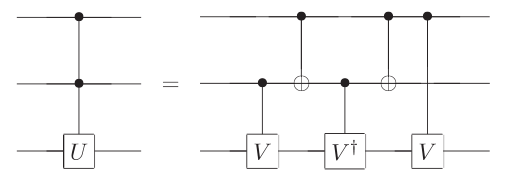
\includegraphics[width=0.75\linewidth]{Images/c2Utoffoli.png}
    \caption{Circuit for the $C^2(U)$ gate. $V$ is any unitary operator satisfying $ V^2=U$. The special case $V=(1-\iota)(I+\iota X)/2$ corresponds to the Toffoli gate.}
    \label{fig:c2utoff}
\end{figure}
Ultimately we will show that any unitary operation can be composed into an arbitrary good approximation from just the Hadamard, phase, controlled-NOT and $\pi/8$ gates. Because of the great usefulness of the Toffoli gate it is interesting to see how it can be built from just this gate set. Figure \ref{fig:toffdecomp} illustrates a simple circuit for the Toffoli gate made up of just Hadamard, phase, controlled-NOT and $pi/8$ gates.
\begin{figure}[ht]
    \centering
    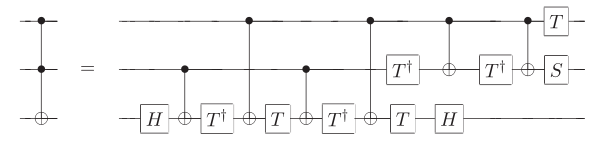
\includegraphics[width=1\linewidth]{Images/toffoli_decomp.png}
    \caption{Implementation of the Toffoli gate using Hadamard, phase, controlled-NOT and $\pi/8$ gates}
    \label{fig:toffdecomp}
\end{figure}

How may we implement $C^n(U)$ gates using our existing repertoire of gates where $U$ is an arbitrary single qubit unitary operation? A particularly simple circuit for achieving this task is illustrated in figure \ref{fig:controlnu}. The circuit divides up into three stages and makes use of a small number $(n-1)$ working qubits, which all start and end in the state $\ket{0}$. Suppose the control qubits are in the computational basis state $\ket{c_1,c_2,\ldots,c_n}$. The first stage of the circuit is to reversible ANd all the control bits $c_1,\ldots,c_n$ together to produce the product $c)1\cdot c_2 \ldots c_n$. To do this, the first gate in the circuit ANDs $c_1$ and $c_2$ together, using a Toffoli gate, changing the state of the first work qubit to $\ket{c_1\cdot c_2}$. The next Toffoli gate ANDs $c_3$ with the product $c_1 \cdot c_2$, changing the state of the second work qubit to $\ket{c_1\cdot c_2 \cdot c_3}$. We continue applying Toffoli gates in this fashion, until the final work qubit is in the state $\ket{c_1 \cdot c_2\ldots c_n}$. Next, a $U$ operation on the target qubit is performed, conditional on the final work qubit being set to one. That is, $U$ is applied if and only if all of $c_1$ through $c_n$ are set. Finally, the last part of the circuit just reverses the steps of the first stage, returning all the work qubits to their initial state, $\ket{0}$. The combined result, therefore, is to apply the unitary operator $U$ to the target qubit, if and only if all the control bits $c_1$ through $c_n$ are set, as desired.
\begin{figure}[ht]
    \centering
    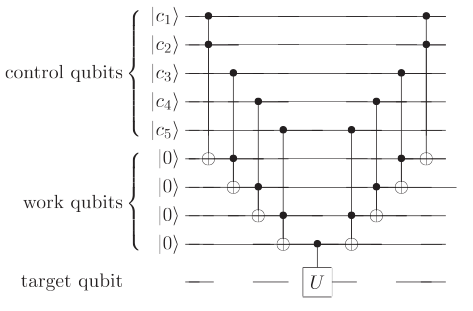
\includegraphics[width=1\linewidth]{Images/controlnu.png}
    \caption{Network implementing the $C^n(U)$ operation for the case, $n=5$}
    \label{fig:controlnu}
\end{figure}
In the controlled gates we have been considering, conditional dynamics on the target qubit occurs if the control bits are set to one. Of course, there is nothing special about one, and it is often useful to consider dynamics which occurs conditional on the control bits being set to zero. For instance, suppose we wish to implement a two qubit gate in which the second (`target') qubit is flipped, conditional on the first (`control') qubit being set to zero. In figure \ref{fig:controldecomp} we introduce a circuit notation for this gate, together with an equivalent circuit in terms of the gates we have already introduced. Generically we shall use the open circle notation to indicate condition on the qubit being set to zero, while a closed circle indicates conditioning on the qubit being set to one.
\begin{figure}[ht]
    \centering
    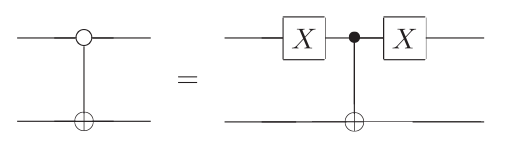
\includegraphics[width=1\linewidth]{Images/controlxdecomp.png}
    \caption{Controlled operation with a NOT gate being performed on the second qubit, conditional on the first qubit being set to zero}
    \label{fig:controldecomp}
\end{figure}
A more elaborate example of this connection, involving three control qubits, is illustrated in figure \ref{fig:cuequiv}. The operation $U$ is applied to the target qubit if the first and third qubits are set to zero, and the second qubit is set to one. It is easy to verify by inspection that the circuit on the right hand side of the figure implements the desired operation. More generally, it is easy to move between circuits which condition on qubits being set to one and circuit which condition on qubits being set to zero, by insertion of $X$ gates in appropriate locations, as illustrated in figure \ref{fig:cuequiv}.
\begin{figure}[ht]
    \centering
    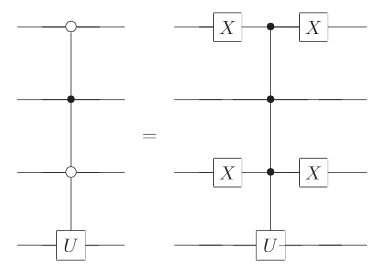
\includegraphics[width=1\linewidth]{Images/cuequiv.png}
    \caption{Controlled-$U$ operation and its equivalent in terms of circuit elements we already know how to implement. The fourth qubit has $U$ applied if the first and third qubits are set to zero, and the second qubit is set to one.}
    \label{fig:cuequiv}
\end{figure}
Another convention which sometimes is useful is to allow the controlled-NOT gates to have multiple targets as shown in figure \ref{fig:multitargetcnot}. This natural notation means that when the control qubit is $1$, then all the qubits marked with a $\oplus$ are flipped, and otherwise nothing happens. It is convenient to use, for example, in construction classical functions such as permutations, or in encodes and decodes for quantum error-correction circuits, as we shall later see.
\begin{figure}[ht]
    \centering
    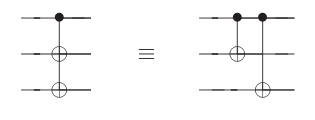
\includegraphics[width=0.5\linewidth]{Images/multiplegatescontrollednot.png}
    \caption{Controlled-NOT gate with multiple targets}
    \label{fig:multitargetcnot}
\end{figure}

\section{Universal quantum gates}
A small set of gates (e.g. AND, OR, NOT) can be used to compute an arbitrary classical functions. We say that such a set of gates is universal for classical computation. In fact, since the Toffoli gate is universal for classical computation, quantum circuits subsume classical circuits. A similar universality is true for quantum computation, where a set of gates is said to be universal for quantum computation if any unitary operation may be approximated to arbitrary accuracy by a quantum circuit involving only those gates. We now describe three universality constructions for quantum computation. These constructions build upon each other, and culminate a proof that any unitary operation can be approximated to arbitrary accuracy using Hadamard, phase, CNOT, and $\pi/8$ gates. You may wonder why the phase gate appears in this list, since it can be constructed from two $\pi/8$ gates; it is included because of its natural role in fault-tolerant constructions described later.

The first construction shows that any arbitrary unitary operator may be expressed exactly as a product of unitary operators that each acts non-trivially only on a subspace spanned by two computational basis states. The second construction combines the first construction with the results of the previous section to show that an arbitrary unitary operator may be expressed exactly using single qubit and CNOT gates. The third construction combines the second construction with a proof that single qubit operation may be approximated to arbitrary accuracy using the Hadamard, phase, and $\pi/8$ gates. This in turn implies that any unitary operation can be approximated to arbitrary accuracy using Hadamard, phase, CNOT and $\pi/8$ gates.

Our construction say little about efficiency - how many (polynomially or exponentially many) gates must be composed in order to create a given unitary transform. Later we show that there exist unitary transforms which require exponentially many gates to approximate. Of course, the goal of quantum computation is to find interesting families of unitary transformations that can be performed efficiently.

\begin{example}
    Construct a quantum circuit to add two two-bit numbers $x$ and $y$ modulo $4$. That is, the circuit should perform the transformation $\ket{x,y} \rightarrow \ket{x,x+y \text{ mod } 4}$.
\end{example}

\subsection{Two-level unitary gates are universal}
Consider a Unitary matrix which acts on a $d$-dimensional Hilbert space. In this section we explain how $U$ may be decomposed into a product of two-level unitary matrices; that is, unitary matrices which act non-trivially only on two-or-fewer vector components. The essential behind this decomposition may be understood by considering the case when $U$ is $3\times 3$ , so suppose $U$ has the form
\[
U=\begin{bmatrix} a & d & g \\ b & c & h \\ c & f & j \end{bmatrix}
\]
We will find two-level unitary matrices $U_1,\ldots,U_3$ such that
\[
U_3U_2U_1U=I
\]
It follows that
\[
U=U_1^{\dagger}U_2^{\dagger}U_3^{\dagger}
\]
$U_1,U_2$ and $U_3$ are all two-level unitary matrices, and it is easy to see that their inverses, $U_1^{\dagger},U_2^{\dagger}$ and $U_3^{\dagger}$ are also two-level unitary matrices. Thus, if we can demonstrate the above equations then we will have shown how to break $U$ into a product of two-level unitary matrices.
Use the following procedure to construct $U_1$; if $b=0$ then set
\[
U_1=\begin{bmatrix}
    1 & 0 & 0 \\ 0 & 1 & 0 \\ 0 & 0 & 1
\end{bmatrix}
\]
If $b\neq 0$ then set
\[
U_1 = \begin{bmatrix} \frac{a^*}{\sqrt{|a|^2+|b|^2}} & \frac{b^*}{\sqrt{|a|^2+|b|^2}}& 0 \\
\frac{b}{sqrt{|a|^2+|b|^2}} & \frac{-a}{\sqrt{|a|^2 + |b|^2}} & 0 \\ 0  & 0 & 1 \end{bmatrix}
\]
Note that in either case $U_1$ is a two-level unitary matrix, and we multiply the matrices out we get
\[
U_1U= \begin{bmatrix} a' & d' & g' \\ 0 & e' & h' \\ c' & f' & j' \end{bmatrix}
\]

The key point to note is that the middle entry in the left hand column is zero. We denote the other entries in the matrix with a generic prime '; their actually values do not matter.

Now apply a similar procedure to find a two-level matrix $U_2$ such that $U_2U_1U$ has no entry in the bottom left corner. That is, if $c'=0$ we set
\[
U_2 = \begin{bmatrix} a'' & 0 & 0 \\ 0 & 1 & 0 \\ 0 & 0 & 1 \end{bmatrix}
\]
while if $c''\neq 0$ then we set
\[
\begin{bmatrix}
\frac{a''}{\sqrt{|a'|^2 + |c'|^2}} & 0 & \frac{c''}{\sqrt{|a'|^2 + |c'|^2}}\\
0 & 1 & 0 \\

\frac{c'}{\sqrt{|a'|^2 +|c'|^2}} & 0 & \frac{-a'}{\sqrt{|a'|^2 + |c'|^2}}
\end{bmatrix}
\]
In either case, when we carry out the matrix multiplication we find that
\[
U_2U_1U=\begin{bmatrix} 1 & d''' & g''' \\
0 & e''' & h''' \\ 
0 & f''' & j''' 
\end{bmatrix}
\]
Since $U,U_1,U_2$ are unitary, it follows that $U_2U_1U$ is unitary , and thus $d'''=g'''=0$, since the first row of $U_2U_1U$ must have norm $1$. Finally, set
\[
U_3=\begin{bmatrix}
1& 0 & 0 \\
0 & e'''' & f''''\\
0 & h'''' & j''''
\end{bmatrix}
\]
It is now easy to verify that $U_3U_2U_1U=I$, and thus $U=U_1^{\dagger}U_2^{\dagger}U_3^{\dagger}$, which is a decomposition of $U$ into two-level unitaries.

More generally, suppose $U$ acts on a $d$-dimensional space. Then, in a similar fashion to the $3\times 3$ case, we can find two-level unitary matrices $U_1,\ldots,U_{d-1}$ such that the the matrix $U_{d-1}U_{d-2}\ldots U_1U$ has a one in the top left hand corner, and all zeroes elsewhere in the first row and column. We then repeat this procedure for the $d-1$ by $d-1$ unitary submatrix in the lower righthand corner of $U_{d-1}U_{d-2}\ldots U_1U$, and so on, with the end result that an arbitrary $d\times d$ unitary matrix may be written
\[
U=V_1\ldots V_k
\]
where the matrices $V_i$ are two-level unitary matrices, and $k\leq (d-1)+(d-2)+\ldots +1=d(d-1)/2$.

\begin{example}
    Provide a decompoisition of the transform
    \[
    \begin{bmatrix} 1 & 1 & 1 & 1 \\ 1 & \iota & -1 & -\iota \\
    1 & -1 & 1 & -\iota \\
    1 & -\iota & -1 & \iota \end{bmatrix}
    \]
    into a product of two-level unitaries. This is a special case of the quantum Fourier transform.
\end{example}

A coroallary of the above result is that an arbitrary unitary matrix on an $n$ qubit system may be written as a product of at most $2^{n-1}(2^n-1)$ two-level unitary matrices. For specific unitary matrices it may be possible to find much more efficient decompositions, but as you will now show there exist matrices which cannot be decomposed as a product of fewer than $d-1$ two-level unitary matrices!
\begin{example}
    Prove that there exists a $d\times d$ unitary $U$ which cannot be decomposed as a product of fewer than $d-1$ two level unitary matrices.
\end{example}

\subsection{Single qubit and CNOT gates are universal}
We have just show that an arbitrary unitary matrix on a $d$-dimensional Hilbert space may be written as a product of two-level unitary matrices. Now we show that single qubit and CNOT gates together can be used to implement an arbitrary two-level unitary operation on the state space of $n$ qubits. Combining these results we see that single qubit and CNOT gates can be used to implement an arbitrary unitary operation on $n$ qubits, and therefore are universal for quantum computation.


Suppose $U$ is a two-level unitary matrix on an $n$ qubit quantum computer. Suppose in particular that $U$ acts non-trivially on the space spanned by the computational basis states $\ket{s}$ and $\ket{t}$, where $s=s_1\ldots s_n$ and $t=t_1\ldots t_n$ are the binary expansions for $s$ and $t$. Let $\tilde{U}$ be the non-trivial submatrix of $U$; $\tilde{U}$ can be though of as a unitary operator an a single qubit.

Our immediate goal is to construct a circuit implementing $U$, built from single qubit and CNOT gates. To do this, we need to make use of Gray codes. Suppose we have distinct binary numbers, $s$ and $t$. A Gray code connecting $s$ and $t$ is a sequence of binary numbers, starting with $s$ and concluding with $t$, such that adjacent members of the list differ exactly in one bit. For instance, with $s=101001$ and $t=110011$ we have the Gray code
\begin{align*}
&101001\\
&101011\\
&100011\\
&110011
\end{align*}

Let $g_1$ trough $g_m$ be the elements of a Gray code connecting $s$ and $t$, with $g_1=s$ and $g_m=t$. Note that we can always find a Gray code such that $m\leq n+1$ since $s$ and $t$ can differ in at most $n$ locations.

The basic idea of the quantum circuit implementing $U$ is to perform a sequence of gates effecting the state changes $\ket{g_1}\rightarrow \ket{g_2} \rightarrow \ldots \rightarrow \ket{g_{m-1}}$, then to perform a controlled-$\tilde{U}$ operation, with the target qubit located at the single bit where $g_{m-1}$ and $g_m$ differ, and then to undo the first stage, transforming $\ket{g_{m-1}}\rightarrow\ket{g_{m-2}}\rightarrow \ldots \rightarrow \ket{g_1}$. Each of these steps can be easily implemented using operations developed earlier in this chapter, and the final result is an implementation of $U$.

A more precise description of the implementation is as follows. The first step is to swap the states $\ket{g_1}$ and $\ket{g_2}$. Suppose $g_1$ and $g_2$ differ at the ith digit. Then we accomplish the swap by performing a controlled bit flip on the ith qubit, conditional on the values of the other qubits being identical to those in both $g_1$ and $g_2$. Next we use a controlled operation to swap $\ket{g_2}$ and $\ket{g_3}$. We continue this fashion until we swap $\ket{g_{m-2}}$ with $\ket{g_{m-1}}$. The effect of this sequence of $m-2$ operations is to achieve the operation

\begin{align*}
    \ket{g_1} &\rightarrow \ket{g_{m-1}}\\
    \ket{g_2} &\rightarrow \ket{g_1}\\
    \ket{g_3} &\rightarrow \ket{g_2}\\
    \vdots \\
    \ket{g_{m-1}} &\rightarrow \ket{g_{m-2}}
\end{align*}
All other computational basis states are left unchanged by this sequence of operations. Next, suppose $g_{m-1}$ and $g_{m}$ differ in the $j$th bit. We apply a controlled-$\tilde{U}$ operation with the $j$th qubit as target, conditional on the other qubits having the same values as appear in both $g_m$ and $g_{m-1}$. Finally, we complete the $U$ operation by undoing the swap operations: we swap $\ket{g_{m-1}}$ with $\ket{g_{m-2}}$, then $\ket{g_{m-2}}$ with $\ket{g_{m-3}}$ and so on, until we swap $\ket{g_2}$ with $\ket{g_1}$.

A simple example illustrates the procedure further. Suppose we wish to implement the two-level unitary transformation
\[
U=\begin{bmatrix} 
a & 0 & 0 & 0 & 0 & 0 & 0 & c \\
0 & 1 & 0 & 0 & 0 & 0 & 0 & 0 \\
0 & 0 & 1 & 0 & 0 & 0 & 0 & 0 \\
0 & 0 & 0 & 1 & 0 & 0 & 0 & 0 \\
0 & 0 & 0 & 0 & 1 & 0 & 0 & 0 \\
0 & 0 & 0 & 0 & 0 & 1 & 0 & 0 \\
0 & 0 & 0 & 0 & 0 & 0 & 1 & 0 \\
b & 0 & 0 & 0 & 0 & 0 & 0 & d \\
\end{bmatrix}
\]
Here, $a,b,c$ and $d$ are any complex numbers such that $\tilde{U}=\begin{bmatrix}a & c \\ b & d \end{bmatrix}$ is a unitary matrix.

Notice that $U$ acts non-trivially only on the states $\ket{000}$ and $\ket{111}$. We write a gray code connection $000$ and $111$:

\begin{table}[ht]
    \centering
    \begin{tabular}{ccc}
        A & B & C\\
        0 & 0 & 0\\
        0 & 0 & 1\\
        0 & 1 & 1\\
        1 & 1 & 1\\
    \end{tabular}
\end{table}

From this we read off the required circuit, shown in figure \ref{fig:circimple2level}. The first two gates shuffle the states so that $\ket{000}$ gets swapped with $\ket{011}$. Next, the operation $\tilde{U}$ is applied to the first qubit of the states $\ket{011}$ and $\ket{111}$, conditional on the second and third qubits being in the state $\ket{11}$. Finally, we unshuffle the states, ensuring that $\ket{011}$ gest swapped back with the state $\ket{000}$.
\begin{figure}[ht]
    \centering
    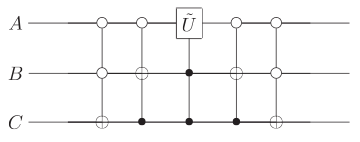
\includegraphics[width=0.75\linewidth]{Images/circuitimp2level.png}
    \caption{Circuit implementing the two-level unitary operation defined}
    \label{fig:circimple2level}
\end{figure}
Returning to the general case, we see that implementing the two-level unitary operation $U$ requires at most $2(n-1)$ controlled operations to swap $\ket{g_1}$ with $\ket{g_{m-1}}$ and then back again. Each of these controlled operations can be realized using $\mathcal{O}(n)$ single qubit and CNOT gates; the controlled-$\tilde{U}$ operation also requires $\mathcal{O}(n)$ gates. Thus, implementing $U$ requires $\mathcal{O}(n^2)$ single qubit and CNOT gates. We saw in the previous section that an arbitrary unitary matrix on the $2^n$ dimensional state space of $n$ qubits may be written as a product of $\mathcal{O}(2^{2n})=\mathcal{O}(4^n)$ two-level unitary operations. Combining these results, we see that an arbitrary unitary operation on $n$ qubits can be implemented using a circuit containing $\mathcal{O}(n^24^n)$ single qubit and CNOT gates. Obviously, this construction does not provide terribly efficient quantum circuits!! However, we will later see that this construction dis close to optimal in the sense that there are unitary operations that require an exponential number of gates to implement. Thus, to find fast quantum algorithm we will clearly need a different approach than is taken in the universality construction. 

\begin{example}
    Find a quantum circuit using single qubit operations and CNOTs to implement the transformation
    \[
    \begin{bmatrix}
        1 & 0 & 0 & 0 & 0 & 0 & 0 & 0 & 0 \\ 
        0 & 1 & 0 & 0 & 0 & 0 & 0 & 0 & 0 \\ 
        0 & 0 & a & 0 & 0 & 0 & 0 & 0 & c \\ 
        0 & 0 & 0 & 1 & 0 & 0 & 0 & 0 & 0 \\ 
        0 & 0 & 0 & 0 & 1 & 0 & 0 & 0 & 0 \\ 
        0 & 0 & 0 & 0 & 0 & 1 & 0 & 0 & 0 \\ 
        0 & 0 & 0 & 0 & 0 & 0 & 1 & 0 & 0 \\ 
        0 & 0 & 0 & 0 & 0 & 0 & 0 & 1 & 0 \\
        0 & 0 & b & 0 & 0 & 0 & 0 & 0 & d \\ 
    \end{bmatrix}
    \]
    where $\tilde{U}=\begin{bmatrix}a & c \\ b & d \end{bmatrix}$ is an arbitrary $2\times 2$ unitary matrix.
\end{example}

\subsection{Approximating arbitrary unitary gates}
Any unitary transformation on any number of qubits can be decomposed as a product of 1- and 2-qubit gates. howeve, if you just run the decomposition blindly, it will produce a quantum circuit with something like $4^n$ gates - just like, if you use the method of truth tables to build a circuit to compute some arbitrary Boolean function, $f:\{0,1\}^n \rightarrow \{0,1\}$, you'll get something with about $2^n$ AND, OR, and NOT gates. Just like in the classical world, our real interest is in which Boolean functions can be efficiently computed - say, using a polynomial number of AND, OR, and NOT gates - so too in the quantum world, our real interest is in which $n$-qubit unitary transformations can be realized using only polynomially many 1 and 2 qubit gates.

That being so, it behooves us to ask: is it possible that all $n$-qubit unitaries can be realized by polynomial-size circuits? The answer turns out to be no. In fact, just like ``almost" all Boolean functions require exponentially large circuits to compute them, so too ``almost all" unitaries require exponentially large quantum circuits. As in the classical case, the way t prove this is using a counting argument.

Counting arguments in circuit complexity go back to Claude Shannon in 1949. Shanon observed that almost every n-bit Boolean function requires a circuit of at least $\sim \frac{2^n}{n}$ AND, OR and NOT (or equivalently NAND) gates to compute it. The reason for this, in one sentences, is that there are too many Boolean functions, and not enough small circuits!! In more detail, there are $2^{2^n}$ different Boolean functions $f:\{0,1\}^n\rightarrow \{0,1\}$. For a circuit with $T$ gates there are $\sim (n+T)^{\mathcal{O}(T)}$ different circuits can be constructed, which can be seen as follows. Without loss of generality suppose we choose to construct out circuit out of NAND gates, with a bounded fan-in of 2. For each NAND gate in our circuit we have
\[
\binom{N+T-1}{2}\leq (N+T)^2
\]
ways to select the inputs. Since there are $T$ gates, the number of different circuits we can construct this way is upper bounded by
\[
(N+T)^{2T}=(N+T)^{\mathcal{O}(T)}
\]
Since each circuit can compute only one function, we can simply set the two expressions eqal and solve for $T$.
\[
2^{2^n} =(n+T)^{T}\approx T^T
\]
Taking the log of both sides gives
\[
2^n = T\log T
\]
This is satisfied for $T\approx \frac{2^n}{n}$. Moreover, if $T$ is smaller then $(N+T)^{\mathcal{O}(T)}$ is minuscule compared to $2^{2^n}$, so almost every function require a circuit of size $\mathcal{O}(\frac{2^n}{n}$.

Strikingly, and famously, this argument doesn't give us a single example of a hard-to-compute Boolean function. It merely tells us that such functions must exist, and indeed are ubiquitous!

We can use a similar sort of argument in the quantum case - although since $2^n\times 2^n$ unitary matrices for a continuous manifold, it's easier to talk in terms of dimensionality rather than cardinality. For simplicity, let's even restrict attention to those $2^n\times 2^n$ unitary matrices that are diagonal. even then, specifying such a matrix clearly requires us to specify $2^n$ independent complex numbers of norm 1 (or $2^n-1$, if we ignore the global phase). By contrast, a quantum circuit with $T$ gates, each acting on at most $2$ qubits, can be specified using only $\mathcal{O}(T)$ continuous parameters (plus some discrete choices about where to apply the gates, which won't affect the argument). So we have a $2^n$-dimensional manifold in the one case, and a union of $\mathcal{O}(T)$-dimensional manifolds in the other. Clearly, for the one to cover the other, we need $T$ to grow at least like $\sim2^n$.Hence, there exist $n$-qubit unitary transformations that require exponentially many gates to implement. In fact, ``almost all" (now in the technical, measure-theory sense of $100\%$ of them) have this property.

You might complaing that we've only showed that exponentially many gates are needed to implement amost $n$-qubit unitary transformations exactly. What about approximately implementing them? That is, implementing them up to small error $\epsilon$ 9say, in each entry)? In fact, a little algebraic geometry is enough to show that exponentially many gates are needed to approximate most $n$-qubit untiaries as well, or even most $n$-qubit diagonal unitary transformations. 

Once again, these arguments don't give us a single example of a hard-to-implement unitary transformation. The easy-to-implement unitaries are the rare exceptions! yet, rare though they might be, the subset of unitaries that are easy (i.e., that can be implemented by polynomial -size quantum circuits) are the main ones that will interest us in quantum computing.

We've seen that any unitary transformation on $n$ qubits can be built up out of a small set of elementary gates. Is it always possible to do this efficiently? That is, given a unitary transformation $U$ on $n$ qubits does there always exist a circuit of size polynomial in $n$ approximating $U$? The answer to this question turns out to be a resounding no: in fact, most unitary transformations can only be implemented very inefficiently. One way to consider the question: how many gates does it take to generate an arbitrary state on $n$ qubits? A simple counting argument shows that this requires exponentially many operations, in general; it immediately follows that there are unitary operations requiring exponentially many operations. to see this, suppose we have $g$ different types of gates available, and each work on at most $f$ qubits. These numbers, $f$ and $g$, are fixed by the computing hardware we have available, and may be considered to be constants. Suppose we have a quantum circuit containing $m$ gates, starting from the computational basis state $\ket{0}^{\otimes n}$. For any particular gate in the circuit there are therefore at most $(\binom{n}{f}))^g=\mathcal{O}(n^{fg})$ possible choices. It follows that at most $\mathcal{O}(n^{fgm})$ different states may be computed using $m$ gates.
\begin{figure}[ht]
    \centering
    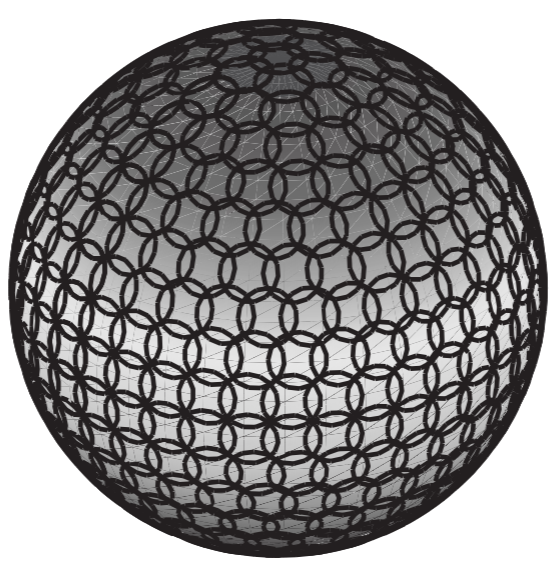
\includegraphics[width=0.5\linewidth]{Images/genericallyhard.png}
    \caption{Visualization of covering the set of possible states with patches of constant radius}
    \label{fig:approxarbgate}
\end{figure}
Suppose we wish to approximate a particular state, $\ket{\psi}$, to within a distance $\epsilon$. The idea of the proof is to cover the set of all possible states with a collection of `patches', each of radius $\epsilon$, and then to show that the number of patches required rises doubly exponentially in $n$; comparing with the exponential number of different states that may be computed using $m$ gates will imply the result. The first observation we need is that the space of state vectors of $N$ qubits can be regarded as just the unit $2^{n+1}-1$ sphere. To see this, suppose the $n$ qubit states has amplitudes $\psi_j = X_j + \iota Y_j$, where $X_j$ and $Y_j$ are the real and imaginary parts, respectively of the $jth$ amplitude. The normalization condition for quantum states can be written $\sum_j (X_j^2 +Y_j^2)=1$, which is just the condition for a point to be on the unit sphere in $2^{n+1}$ real dimensions, that is, the unit $(2^{n+1}-1)$ sphere. Similarly, the surface area od radius $\epsilon$ near $\ket{\psi}$ is the same as the volume of a $(2^{n+1}-2)$ sphere of radius $\epsilon$. Using the formula $S_k(r)=2\pi^{(k+1)/2}r^k/\Gamma ((k+1)/2)$ for the surface area of a $k$-sphere of radius $r$, and $V_k(r)=2\pi^{(k_1)/2}r^{k+1}/[(k+1)\Gamma ((k+1)/2)]$ for the volume of a $k$-sphere of radius $r$, we see that the number of patches needed to cover the space goes like
\[
S_{2^{n+1}-1}(a)=\frac{\sqrt{\pi}\Gamma(2^n-\frac{1}{2})(2^{n+1}-1)}{\Gamma(2^n)\epsilon^{2^{n+1}-1}}
\]
where $\Gamma$ us the usual generalization of the factorial function. But $\Gamma(2^{n-1}/2)\geq \Gamma(2^n)/2^n$, so the number of patches required to cover the space is at least
\[
\Omega\left(\frac{1}{\epsilon^{2^{n+1}-1}}\right)
\]
Recall that the number of patches which can be reached in $m$ gates if $\mathcal{O}(n^{fgm})$, so in order to reach all the $\epsilon$-patches we must have
\[
\mathcal{O}(n^{fgm}) \geq \Omega\left(\frac{1}{\epsilon^{2^{n+1}-1}}\right)
\]
which gives
\[
m=\Omega\left(\frac{2^n\log (1/\epsilon)}{\log(n)}\right)
\]
That is, there are states of $n$ qubits which take $\Omega(2^n\log (1/\epsilon)/\log(n))$ operations to approximate to within a distance $\epsilon$. This is exponential in $n$, and thus is `difficult' , in the sense of computational complexity . Furthermore, this immediately implies that there are unitary transformation on $n$ qubits which take $\Omega(2^n\log(1/\epsilon)/\log(n))$ operations to approximate by a quantum circuit implementing an operation $V$ such that $E(U,V)\leq \epsilon$. By contrast using our universality constructions and the Solovay-Kitaev theorem it follows that an arbitrary unitary operation $U$ on $n$ qubits may be approximated to within a distance $\epsilon$ using $\mathcal{O}(n^2 4^n \log^c(n^2 4^n/\epsilon))$ gates. Thus, to within a polynomial factor the construction for universality we have given is optimal; unfortunately, it does not address the problem of determining which families of unitary operations can be computed efficiently in the quantum circuits model.

\section{Measurements}
A final element used in quantum circuits, almost implicitly sometimes, is measurement. In out circuits, we shall denote a projective measurement in the computational basis using a `meter' symbol as illustrated in figure \ref{fig:meassym}. In the theory of quantum circuits it is conventional to not use any special symbols to denote more general measurements, because, they can always be represented by unitary transformation with ancilla bits followed by projective measurements.
\begin{figure}[ht]
    \centering
    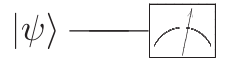
\includegraphics[width=0.5\linewidth]{Images/meassym.png}
    \caption{Symbol for projective measurement on a single qubit. In this circuit nothing further is done with the measurement results, bit in more general quantum circuits  it si possible to change later parts of the quantum circuit, conditional on measurement outcomes in earlier parts of the circuit. Such a usage of classical information is depicted using wires drawn with double lines (not shown here)}
    \label{fig:meassym}
\end{figure}
There are two important principles that is worth bearing in mind about quantum circuits. Both principles are rather obvious; however, they are of such great utility that they are worth emphasizing early. The first principle is that classically conditioned operations can be replaced by quantum conditioned operations:
\subsection{Principle of deferred measurement}
\label{subsec:princ_deffer_meas}
\begin{definition}
    Measurement can always be moved from an intermediate stage of a quantum circuit to the end of the circuit; if the measurement results are used at any stage of the circuit then the classically controlled operations can be replaced by conditional quantum operations.
\end{definition}

Often, quantum measurements are performed as an intermediate step in a quantum circuit, and the measurement results are used to conditionally control subsequent quantum gates. That is the case, for example, in the teleportation circuit of figure \ref{fig:teleportation}. However, such measurements can always be moved to the end of the circuit. Figure \ref{fig:qctele} illustrates how this may be done by replacing all the classical conditional operations by corresponding quantum conditional operations, (Of course, some of the interpretation of this circuit as performing `teleportation' is lost, because no classical information is transmitted from Alice to Bob, but it is clear that the overall action of the two quantum circuit is the same, which is the key point.)
\begin{figure}[ht]
    \centering
    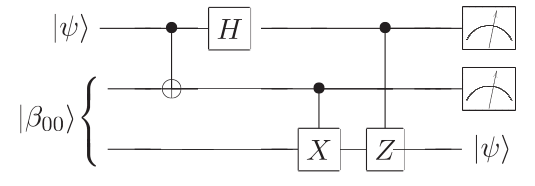
\includegraphics[width=0.75\linewidth]{Images/qcteleport.png}
    \caption{Quantum teleportation circuit in which measurements are done at the end, instead of in the middle of the circuit. The top two qubits belong to Alice, and the bottom one to Bob.}
    \label{fig:qctele}
\end{figure}
The second principle is even more obvious and surprisingly useful!

\subsection{Principle of implicit measurement}
\label{subsec:princ_implicit_meas}
\begin{definition}
    Without loss of generality, any unterminated quantum wires (qubits which are not measured) at the end of a quantum circuit may be assumed to be measured.
\end{definition}
To understand why this is true, imagine you have a quantum circuit containing just two qubits, and only the first qubit is measured at the end of the circuit. Then the measured statistics observed at this time are completely determined by the reduced density matrix of the first qubit. However, if a measurement had also bee performed on the second qubit, then it would be highly surprising if that measurement could cahnge the statistics of the measurement on the first qubit. This is because the reduced density matrix of the first qubit is not affected by performing a measurement on the second.

As you consider the role of measurements in quantum circuits, it is important to keep in mind that in its role s an interface between the quantum and classical worlds, measurement is generally considered to be an irreversible operation, destroying quantum information and replacing it with classical information. In certain carefully designed cases however, this need not be true, as is vividly illustrated by teleportation and quantum error-correction. What teleportation and quantum-error correction have in common is that in neither instance does the measurement reveal any information about the identity of the quantum state being measured, Indeed, we will see in a later chapter that this is a more general feature of measurement - in order for a measurement to be reversible, it must reveal no information about the quantum state being measured!

\begin{example}
    Suppose $\rho$ is the denisty matrix describing a two qubit system. Suppose we perfomr a projective measurement in the computational basis of the second qubit. Let $P_0\ket{0}\bra{0}$ and $P_1=\ket{1}\bra{1}$ be the projectors onto the $\ket{0}$ and $\ket{1}$ states of the second qubit, respectively. Let $\rho'$ be the density matrix which would be assigned to the system after the measurement by an observed who did not learn measurement result. Show that
    \[
    \rho'=P_0\rho P_0 + P_1 \rho P_1
    \]
    Also show that the reduced density matrix for the first qubit is not affected by the measurement, that is, $tr(\rho)=tr(\rho')$.
\end{example}

\begin{example}
\textbf{(Measurement in Bell basis)} The measurement model we have specified for the quantum circuit model is that measurements are performed only in the computational basis. However, often we want to perform a measurement in some other basis, defined by a complete set of orthonormal states. To perform this measurement, simply unitarily transform from the basis we wish to perform the measurement in to the computational basis, then measure, For example, show that the circuit

performs a measurement in the basis of Bell states. More precisely, show that this circuit results in a measurement being performed with corresponding POVM elements the four projectors onto the Bell states. What are the correspodning measurement operators.
\end{example}


\begin{example}
    \textbf{(Measuring an operator)} Suppose we have a single qubit operator $U$ with eigenvalues $\pm1$ so that $U$ is both Hermitian and unitary, os it can be regarded both as an observable and a quantum gate. Suppose we wish to measure the observable $U$. That is, we desire to obtain a measurement result indicating one of the two eigenvalues, and leaving a post measurement state which is the corresponding eigenvector. How can this be implementing by a quantum circuit? Show that the following circuit implements a measurement of $U$:
\end{example}

\begin{example}
    \textbf{(Measurement commuted with controls)} A consequence of the principle of deferred measurement is that the measurements commute with quantum gates when the qubit being measured is a control qubit, that is:

    
(Recall that double lines represent classical bits in this diagram). Prove the first equality. The rightmost circuit is simply a convenient notation to depict the use of a measurement result to classically control a quantum gate.
\end{example}





